\documentclass[a4paper,11pt]{book}
%\documentclass[a4paper,twoside,11pt,titlepage]{book}
\usepackage{listings}
\usepackage[utf8]{inputenc}
\usepackage[spanish]{babel}

% \usepackage[style=list, number=none]{glossary} %
%\usepackage{titlesec}
%\usepackage{pailatino}

\decimalpoint
\usepackage{dcolumn}
\newcolumntype{.}{D{.}{\esperiod}{-1}}
\makeatletter
\addto\shorthandsspanish{\let\esperiod\es@period@code}
\makeatother


%\usepackage[chapter]{algorithm}
\RequirePackage{verbatim}
%\RequirePackage[Glenn]{fncychap}
\usepackage{fancyhdr}
\usepackage{graphicx}
\usepackage{afterpage}

\usepackage{subcaption}
\usepackage{rotating}

\usepackage[normalem]{ulem}
\useunder{\uline}{\ul}{}

\usepackage{float}
\usepackage[spanish,onelanguage]{algorithm2e} %for psuedo code

% Math style letters
\usepackage{amsfonts}
\usepackage{amsmath}
\usepackage{amssymb}

\usepackage{longtable}
\usepackage{tikz}

\usepackage[pdfborder={000},hidelinks]{hyperref} %referencia


%%%%%%%%%%%%%%%%%%%%%%%%%%%%%%%%%%%%%%%%%%%%%%%%%%%%%%%%%%%%%%%%%%%%%%%%%%%%%%%%%%%%%%%%%%%%%%%%%%
%%                                 Para codigo python                                           %%
%%%%%%%%%%%%%%%%%%%%%%%%%%%%%%%%%%%%%%%%%%%%%%%%%%%%%%%%%%%%%%%%%%%%%%%%%%%%%%%%%%%%%%%%%%%%%%%%%%

\usepackage{color}
\usepackage{listings}
\usepackage{setspace}
\definecolor{Code}{rgb}{0,0,0}
\definecolor{Decorators}{rgb}{0.5,0.5,0.5}
\definecolor{Numbers}{rgb}{0.5,0,0}
\definecolor{MatchingBrackets}{rgb}{0.25,0.5,0.5}
\definecolor{Keywords}{rgb}{0,0,1}
\definecolor{self}{rgb}{1,0,0.5}
\definecolor{Strings}{rgb}{0,0.63,0}
\definecolor{Comments}{rgb}{0,0.63,1}
\definecolor{Backquotes}{rgb}{0,0,0}
\definecolor{Classname}{rgb}{1,0,0.5}
\definecolor{FunctionName}{rgb}{0,0,1}
\definecolor{Operators}{rgb}{1,0,0.5}
\definecolor{Background}{rgb}{0.98,0.98,0.98}
\lstdefinelanguage{Python}{
	numbers=left,
	numberstyle=\footnotesize,
	numbersep=1em,
	xleftmargin=1em,
	framextopmargin=2em,
	framexbottommargin=2em,
	showspaces=false,
	showtabs=false,
	showstringspaces=false,
	frame=l,
	tabsize=4,
	% Basic
	basicstyle=\ttfamily\small\setstretch{1},
	backgroundcolor=\color{Background},
	% Comments
	commentstyle=\color{Comments}\sffamily,
	% Strings
	stringstyle=\color{Strings},
	morecomment=[s][\color{Strings}]{"""}{"""},
	morecomment=[s][\color{Strings}]{'''}{'''},
	% keywords
	morekeywords={import,from,class,def,for,while,if,is,in,elif,else,not,and,or,print,break,continue,return,True,False,None,access,as,,del,except,exec,finally,global,import,lambda,pass,print,raise,try,assert},
	keywordstyle={\color{Keywords}\bfseries},
	% additional keywords
	morekeywords={[2]@invariant,pylab,numpy,np,scipy},
	keywordstyle={[2]\color{Decorators}\slshape},
	emph={self},
	emphstyle={\color{self}\slshape},
	%
}

%%%%%%%%%%%%%%%%%%%%%%%%%%%%%%%%%%%%%%%%%%%%%%%%%%%%%%%%%%%%%%%%%%%%%%%%%%%%%%%%%%%%%%%%%%%%%%%%%%

% ********************************************************************
% Re-usable information
% ********************************************************************
%\newcommand{\myTitle}{Biblioteca de algoritmos de detección de anomalías basados en técnicas de ensembles\xspace}
%\newcommand{\myDegree}{Doble grado Ingeniería Informática y Matemáticas\xspace}
%\newcommand{\myName}{Ignacio Aguilera Martos\xspace}
%\newcommand{\myProf}{Francisco Herrera Triguero\xspace}
%%\newcommand{\mySupervisor}{Put name here\xspace}
%\newcommand{\myFaculty}{Escuela Técnica Superior de Ingenierías Informática y de
%Telecomunicación y Facultad de Ciencias\xspace}
%\newcommand{\myFacultyShort}{E.T.S. de Ingenierías Informática y de
%Telecomunicación y Facultad de Ciencias\xspace}
%\newcommand{\myDepartment}{Departamento de Ciencias de la Computación e Inteligencia Artificial\xspace}
%\newcommand{\myUni}{\protect{Universidad de Granada}\xspace}
%\newcommand{\myLocation}{Granada\xspace}
%\newcommand{\myTime}{\today\xspace}
%\newcommand{\myVersion}{Version 0.1\xspace}
%
%
%\hypersetup{
%pdfauthor = {\myName (nacheteam@correo.ugr.es)},
%pdftitle = {\myTitle},
%pdfsubject = {},
%pdfkeywords = {outlier, anomalía, ensemble},
%pdfcreator = {LaTeX},
%pdfproducer = {pdflatex}
%}


%\hyphenation{}


%\usepackage{doxygen/doxygen}
%\usepackage{pdfpages}
\usepackage{url}
\usepackage{colortbl,longtable}
\usepackage[stable]{footmisc}
%\usepackage{index}

%\makeindex
%\usepackage[style=long, cols=2,border=plain,toc=true,number=none]{glossary}
% \makeglossary

% Definición de comandos que me son tiles:
%\renewcommand{\indexname}{Índice alfabético}
%\renewcommand{\glossaryname}{Glosario}

\pagestyle{fancy}
\fancyhf{}
\fancyhead[LO]{\leftmark}
\fancyhead[RE]{\rightmark}
\fancyhead[RO,LE]{\textbf{\thepage}}
\renewcommand{\chaptermark}[1]{\markboth{\textbf{#1}}{}}
\renewcommand{\sectionmark}[1]{\markright{\textbf{\thesection. #1}}}

\setlength{\headheight}{1.5\headheight}

\newcommand{\HRule}{\rule{\linewidth}{0.5mm}}
%Definimos los tipos teorema, ejemplo y definición podremos usar estos tipos
%simplemente poniendo \begin{teorema} \end{teorema} ...
\newtheorem{teorema}{Teorema}[chapter]
\newtheorem{proposicion}{Proposición}[chapter]
\newtheorem{propiedad}{Propiedad}[chapter]
\newtheorem{lema}{Lema}[chapter]
\newtheorem{demostracion}{Demostración}[chapter]
\newtheorem{propiedades}{Propiedades}[chapter]
\newtheorem{ejemplo}{Ejemplo}[chapter]
\newtheorem{definicion}{Definición}[chapter]

\newcommand*{\QEDA}{\hfill\ensuremath{\blacksquare}}%
\newcommand*{\QEDB}{\hfill\ensuremath{\square}}%

\definecolor{gray97}{gray}{.97}
\definecolor{gray75}{gray}{.75}
\definecolor{gray45}{gray}{.45}
\definecolor{gray30}{gray}{.94}

\lstset{ frame=Ltb,
     framerule=0.5pt,
     aboveskip=0.5cm,
     framextopmargin=3pt,
     framexbottommargin=3pt,
     framexleftmargin=0.1cm,
     framesep=0pt,
     rulesep=.4pt,
     backgroundcolor=\color{gray97},
     rulesepcolor=\color{black},
     %
     stringstyle=\ttfamily,
     showstringspaces = false,
     basicstyle=\scriptsize\ttfamily,
     commentstyle=\color{gray45},
     keywordstyle=\bfseries,
     %
     numbers=left,
     numbersep=6pt,
     numberstyle=\tiny,
     numberfirstline = false,
     breaklines=true,
   }
 
% minimizar fragmentado de listados
\lstnewenvironment{listing}[1][]
   {\lstset{#1}\pagebreak[0]}{\pagebreak[0]}

\lstdefinestyle{CodigoC}
   {
	basicstyle=\scriptsize,
	frame=single,
	language=C,
	numbers=left
   }
\lstdefinestyle{CodigoC++}
   {
	basicstyle=\small,
	frame=single,
	backgroundcolor=\color{gray30},
	language=C++,
	numbers=left
   }

 
\lstdefinestyle{Consola}
   {basicstyle=\scriptsize\bf\ttfamily,
    backgroundcolor=\color{gray30},
    frame=single,
    numbers=none
   }


\newcommand{\bigrule}{\titlerule[0.5mm]}


%Para conseguir que en las páginas en blanco no ponga cabecerass
\makeatletter
\def\clearpage{%
  \ifvmode
    \ifnum \@dbltopnum =\m@ne
      \ifdim \pagetotal <\topskip
        \hbox{}
      \fi
    \fi
  \fi
  \newpage
  \thispagestyle{empty}
  \write\m@ne{}
  \vbox{}
  \penalty -\@Mi
}
\makeatother

\usepackage{pdfpages}
\begin{document}
\setlength{\parskip}{10pt}

\begin{titlepage}
 
 
\newlength{\centeroffset}
\setlength{\centeroffset}{-0.5\oddsidemargin}
\addtolength{\centeroffset}{0.5\evensidemargin}
\thispagestyle{empty}

\noindent\hspace*{\centeroffset}\begin{minipage}{\textwidth}

\centering

\includegraphics[width=0.9\textwidth]{imagenes/logos/logo_ugr.jpg}\\[1.4cm]

\textsc{ \Large TRABAJO FIN DE MÁSTER\\[0.2cm]}
\textsc{ Máster Oficial en Ciencia de Datos e Ingeniería de Computadores}\\[1cm]
% Upper part of the page
% 
% Title
{\Huge\bfseries Detección de Anomalías en Series Temporales basada en técnicas Deep Learning\\
}
\noindent\rule[-1ex]{\textwidth}{3pt}\\[3.5ex]
{\large\bfseries Biblioteca de algoritmos}
\end{minipage}

\vspace{2.5cm}
\noindent\hspace*{\centeroffset}\begin{minipage}{\textwidth}
\centering

\textbf{Autor}\\ {Ignacio Aguilera Martos}\\[2.5ex]
\textbf{Director}\\
{Francisco Herrera Triguero}\\[2cm]

\includegraphics[width=0.3\textwidth]{imagenes/logos/etsiit_logo.png}\\[0.1cm]
\textsc{Escuela Técnica Superior de Ingenierías Informática y de Telecomunicación}\\

\includegraphics[width=0.2\textwidth]{imagenes/logos/ciencias.png}\\[0.1cm]
\textsc{Facultad de Ciencias}\\
\textsc{---}\\
Granada, 10 de Septiembre de 2020
\end{minipage}
%\addtolength{\textwidth}{\centeroffset}
%\vspace{\stretch{2}}
\end{titlepage}



\chapter*{}
%\thispagestyle{empty}
%\cleardoublepage

%\thispagestyle{empty}

\begin{titlepage}
 
 
\setlength{\centeroffset}{-0.5\oddsidemargin}
\addtolength{\centeroffset}{0.5\evensidemargin}
\thispagestyle{empty}

\noindent\hspace*{\centeroffset}\begin{minipage}{\textwidth}

\centering
%
\includegraphics[width=0.9\textwidth]{imagenes/logo_ugr.jpg}\\[1.4cm]

%\textsc{ \Large PROYECTO FIN DE CARRERA\\[0.2cm]}
%\textsc{ INGENIERÍA EN INFORMÁTICA}\\[1cm]
% Upper part of the page
% 

 \vspace{3.3cm}

%si el proyecto tiene logo poner aquí
%
\includegraphics{imagenes/logo.png} 
% \vspace{0.5cm}

% Title

{\Huge\bfseries Detección de Anomalías en Series Temporales basada en técnicas Deep Learning\\
}
\noindent\rule[-1ex]{\textwidth}{3pt}\\[3.5ex]
{\large\bfseries Biblioteca de algoritmos\\[4cm]}
\end{minipage}

\vspace{2.5cm}
\noindent\hspace*{\centeroffset}\begin{minipage}{\textwidth}
\centering

\textbf{Autor}\\ {Ignacio Aguilera Martos}\\[2.5ex]
\textbf{Directores}\\
{Francisco Herrera Triguero}\\[2cm]
%
\includegraphics[width=0.15\textwidth]{imagenes/tstc.png}\\[0.1cm]
%\textsc{Departamento de Teoría de la Señal, Telemática y Comunicaciones}\\
%\textsc{---}\\
%Granada, mes de 201
\end{minipage}
%\addtolength{\textwidth}{\centeroffset}
\vspace{\stretch{2}}

 
\end{titlepage}






\cleardoublepage
\thispagestyle{empty}

\begin{center}
{\large\bfseries Detección de Anomalías en Series Temporales basada en técnicas Deep Learning: Biblioteca de algoritmos}\\
\end{center}
\begin{center}
Ignacio Aguilera Martos\\
\end{center}

%\vspace{0.7cm}
\noindent{\textbf{Palabras clave}: % RELLENAR CON LAS PALABRAS CLAVE EN ESPAÑOL
			}\\

\vspace{0.7cm}
\noindent{\textbf{Resumen}}\\

% RELLENAR CON EL ABSTRACT EN ESPAÑOL

\cleardoublepage


\thispagestyle{empty}


\begin{center}
{\large\bfseries Outlier Detection in Time Series using Deep Learning: Library implementation}\\
\end{center}
\begin{center}
Ignacio Aguilera Martos\\
\end{center}

%\vspace{0.7cm}
\noindent{\textbf{Keywords}: % RELLENAR CON LAS PALABRAS CLAVE EN INGLES
			}\\

\vspace{0.7cm}
\noindent{\textbf{Abstract}}\\

% RELLENAR CON EL ABSTRACT EN INGLES

\chapter*{Agradecimientos}
\thispagestyle{empty}

% RELLENAR CON LOS AGRADECIMIENTOS EN ESPAÑOL
\frontmatter
\tableofcontents
%\listoffigures
%\listoftables
%
\mainmatter

\chapter{Introducción}
\label{chapter:introduccion}
\markboth{Introducción}{}
\pagenumbering{arabic}
\setcounter{page}{1}

Antes de comenzar con el desarrollo en sí del estudio acometido en este trabajo, vamos a contextualizar el mismo y vamos a establecer un marco de trabajo teórico previo a la experimentación, que nos otorgará de rigurosidad para la parte práctica del mismo.

El estudio realizado en este trabajo versa sobre la aplicación de estructuras de Aprendizaje Profundo (Deep Learning) para obtención y detección de anomalías, en concreto, en series temporales. Dentro de este trabajo se van a desarrollar las técnicas conocidas como Autoencoders y Redes Neuronales para predicción de series temporales.

Lo primero que atacaremos en este estudio es la definición de anomalía, para luego pasar a una introducción teórica de Estadística Multivariante y Machine Learning en general. Estas dos secciones nos van a aportar el rigor que necesitamos para adentrarnos teóricamente dentro del Deep Learning y entender los fundamentos de las arquitecturas de redes neuronales que aplicaremos en la práctica.

Tras esto se realizará una descripción de la experimentación realizada, los datos que se emplearán en dicha experimentación y los resultados de la misma. 

%%%%%%%%%%%%%%%%%%%%%%%%%%%%%%%%%%%%%%%%%%%%%%%%%

\section{Contextualización}

Lo primero que debemos de hacer antes de empezar, es establecer el problema u objetivo a resolver de este estudio. Para ello vamos a hacer una breve introducción a los datos (o al problema propuesto que es lo mismo en este ámbito) y a explicar por qué precisamos de un trabajo arduo y prolongado, es decir, por qué no es un problema trivial.

\subsection{Definición del problema}

El ámbito de trabajo va a ser el de las series temporales, pues el conjunto de datos que nos define el problema es una serie temporal. Esta serie temporal mide la sensórica de una máquina de la empresa ArcelorMittal, que no podemos especificar por motivos de privacidad. En este sentido tenemos 106 variables de tipo numérico con las que vamos a trabajar y 468 días de datos con una granularidad de una medida por segundo. Esto hace que el volumen de datos del que disponemos sea inmenso, haciendo que tenga sentido el uso del Deep Learning por la enorme cantidad de datos de entrenamiento de los que vamos a disponer.

Como hemos comentado los datos son medidas de sensores de una cierta máquina. Esta máquina experimenta errores graves de vez en cuando, que hacen que se deba detener completamente para labores de mantenimiento. Nuestro objetivo es ser capaces de detectar estas labores de mantenimiento mediante técnicas de detección de anomalías. El principio subyacente es sencillo: esperamos un comportamiento normal de la máquina en la mayoría del tiempo salvo cuando haya necesidad de un mantenimiento, momento en el cual la sensórica arrojará medidas alteradas que nos den pie a pensar en un posible fallo.

Este tipo de problemas son conocidos como mantenimiento predictivo, pues lo que pretenden precisamente es anticipar la necesidad de dichas labores.

Con esto dicho nuestro objetivo será tomar los datos de entrada (la sensórica) para nuestros modelos Deep Learning y, de alguna manera, saber diferenciar lo que son datos normales y datos anómalos.

\section{Contenido básico y fuentes}

% REVISAR CUANDO TERMINE EL CONTENIDO %

El trabajo contiene una primera sección en la que se incluye una introducción de Aprendizaje Automático orientado específicamente a nuestro problema. Para ello primero se hace una contextualización del concepto de aprendizaje así como los principios inductivos que guían el mismo hacia un buen resultado como por ejemplo el ERM o minimización del error empírico. Se aportan también algunas reflexiones y conceptos en cuanto a la aproximación de funciones, que no es más que el objetivo del aprendizaje automático. 

Todos estos conocimientos están basados en la teoría estadística de Vapnik y Chervonenkis que es brevemente repasada y en la que se dan cotas sobre el aprendizaje y su rendimiento. Esta introducción ha sido escrita basándose en tres libros: Learning from Data de Yaser Abu-Mostafa \cite{yaser_learning_2012}, Learning from Data de Cherkassky y Mulier \cite{cherkassky_learning_2007}  y Outlier Ensembles de Aggarwal y Sathe \cite{aggarwal_outlier_2017}.

Este marco nos dirige hacia la primera definición del concepto de anomalía que está basada en distancias y rangos intercuartil que se describen en el libro Outlier Analysis \cite{aggarwal_outlier_2017-1}. Además se introduce el tipo de datos que vamos a encontrar en el marco del estudio: las series temporales.

Para dar una definición alternativa y una buena base teórica para los modelos debemos hacer una breve introducción estadística. En esta introducción se define un vector aleatorio así como su función de densidad, su función característica y su función de distribución. Se refieren los conceptos de independencia y probabilidad y esperanza condicionada. Por último y aprovechando este contexto se enuncian y demuestran algunas desigualdades y fórmulas famosas. Este contenido viene dado por los apuntes de la asignatura Estadística Multivariante del grado en Matemáticas, los apuntes de la asignatura Procesos Estocásticos del grado en Matemáticas y el libro Probability Theory de M. Loève \cite{m._loeve_probability_1977}.

Tras esto puede ser introducido el concepto probabilístico y basado en densidad de una anomalía. Este concepto viene apoyado en el paper \cite{fabian_keller_hics:_2012} que describe el algoritmo HICS.

Tras este marco teórico de aprendizaje, estadística multivariante y definiciones de anomalías introducimos los conocimientos necesarios de Deep Learning para el desarrollo y entendimiento de los modelos no supervisados implementados. Esta sección hace una revisión de cómo funcionan las redes neuronales, distintos tipos de capas empleados en las arquitecturas implementadas y algunas arquitecturas con mayor fundamentación académica como los Autoencoder. Esta sección se apoya en el libro Deep Learning de Goodfellow, Bengio y Courville \cite{goodfellow_deep_2016}, el libro Deep Learning with Tensorflow de Zaccone, Karim y Menshawy \cite{giancarlo_deep_2017} y la revisión sobre modelos Autoencoder de D. Charte, F. Charte, García, Mª J. del Jesús y F. Herrera \cite{david_practical_2018}.

La siguiente sección analiza y explica los modelos implementados con su código propio. Esta sección se apoya en varios artículos como \cite{lih_oh_automated_2018} o \cite{david_practical_2018} para obtener las arquitecturas empleadas y aplicarlas al ámbito no supervisado que necesitamos.

La siguiente sección explica cómo se integran los algoritmos de detección de anomalías para poder ser empleados para detectar los mantenimientos y cómo obtenemos etiquetas de los datos.

Tras esto se exponen los resultados obtenidos así como la metodología de la experimentación para finalizar con las conclusiones y trabajo futuro derivados del estudio.

\section{Objetivos}

Por todo lo descrito anteriormente el trabajo tiene los siguientes objetivos claros:

\begin{itemize}
	\item Desarrollar un marco teórico sobre el Machine Learning.
	\item Desarrollar un marco teórico sobre el Deep Learning.
	\item Estudiar el estado del arte de los algoritmos de detección de anomalías que emplean Deep Learning.
	\item Estudiar la teoría estadística que rodea el Machine Learning y el Deep Learning.
	\item Entender los fundamentos teóricos y el funcionamiento de los modelos implementados.
	\item Desarrollar una implementación de los modelos.
	\item Obtener una comparativa entre los modelos clásicos y los Deep Learning.
\end{itemize}

Todos estos objetivos han sido alcanzados en el desarrollo de este estudio, obteniendo conclusiones de calidad y líneas de trabajo futuro que se aplicarán a la continuidad del proyecto.
%
\part{Machine Learning, Deep Learning y el concepto de anomalía}
\label{part:machine_learning_deep_learning_anomalia}

\chapter{Concepto de Anomalía y Series Temporales}
\label{chapter:anomalia}

\section{Concepto de Anomalía}

Debemos de tener en cuenta que el concepto de anomalía no es algo fácil de definir. Tanto es así que, por ligeros cambios o matices en la definición, podemos estar cayendo en un concepto completamente distinto.

Antes de comenzar debemos aclarar el objetivo que vamos persiguiendo, es decir, el concepto de anomalía que nos va a interesar. Podemos encontrar muchas definiciones de anomalías, pero en nuestro caso nos vamos a centrar en la dada por Carreño, Inza y Lozano en \cite{ander_analyzing_2019}.

Según estos autores podemos definir el contexto de la detección de anomalías en 4 subtipos: eventos raros, anomalías, novedades y outliers. 

En primer lugar, tenemos los eventos raros. Tenemos un problema en el que hay un tipo de datos que aparecen con muy poca frecuencia en el contexto de las series temporales y queremos detectar dicho tipo de eventos. Estamos en una perspectiva supervisada, por lo que esto no es más que un problema de clasificación altamente desbalanceado en el contexto de las series temporales. En este escenario el problema se resuelve aplicando distintas técnicas que favorezcan que los clasificadores aprendan bien esta clase rara y se detecte. Claramente no es nuestro caso pues no disponemos de etiquetas claras y no es un problema de clasificación.

En segundo lugar tenemos las anomalías. Según Carreño, las anomalías están enmarcadas en conjuntos de datos estáticos. Este simple hecho ya saca el subtipo de nuestro marco de trabajo, pero aún así es bueno ver su definición. Las anomalías son, para Carreño et al., un problema de clasificación altamente desbalanceado en el contexto de datos estáticos. Esto es análogo al caso anterior, salvando el paso de datos estáticos a dinámicos. Claramente no es nuestro caso pues el problema no es de clasificación ni tenemos etiquetas claras ni son datos estáticos de los que disponemos.

En tercer lugar tenemos las novedades. Este apartado puede ser aplicado tanto a datos estáticos como a datos dinámicos. En los dos casos anteriores tenemos problemas de clasificación, pero disponemos de las etiquetas y de ejemplos de todas las clases para la fase de entrenamiento. En las novedades tenemos datos normales de una sola clase en la fase de entrenamiento, por lo que en el momento de entrenar tendremos que definir las fronteras de la única clase que tenemos. El objetivo en este problema es detectar la novedad, es decir, los nuevos ejemplos que no cuadran dentro de la frontera de decisión de la única clase que tenemos en la fase de entrenamiento en el problema. De nuevo esto no es nuestro caso, porque no tenemos etiquetas de los datos normales y por tanto no podemos definir claramente ese marco de trabajo ``one class''.

Por último tenemos los outliers. Este término no es de fácil traducción al español, por lo que es preferible dejar el original en inglés. Este punto engloba la clasificación no supervisada, es decir, tenemos ciertas nociones del conjunto de datos pero ninguna etiqueta precisa y aun así queremos saber qué datos son normales y cuáles anómalos basándonos en alguna técnica que no emplee más que los propios datos sin etiquetar. Este es nuestro marco de trabajo, pues no disponemos de etiquetas claras ni ``ground truth'', oráculo o verdad absoluta a la que recurrir para aprender de ella. Tenemos que elaborar un sistema capaz de detectar los mantenimientos de nuestra máquina sin poder aprender a priori lo que es normal y lo que es anómalo.

Dentro de este esquema de posibilidades ya hemos localizado la que más se acerca al objetivo que queremos cumplir. Como hemos podido ver, es la única opción completamente no supervisada que Carreño contempla en el artículo, lo que nos deja con el escenario más complejo de todos. 

Pensemos un momento todas las posibles definiciones de anomalías que tenemos mediante varios ejemplos.

\begin{figure}[H]
	\centering
	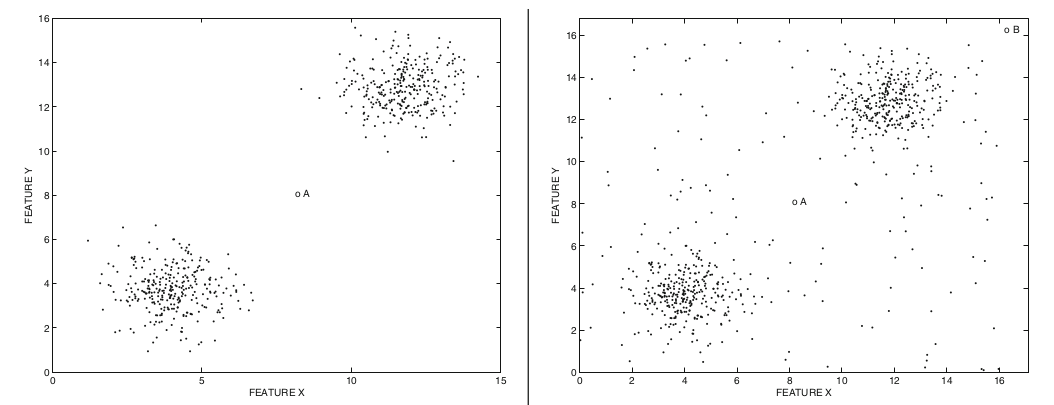
\includegraphics[scale=0.35]{imagenes/ejemplo1_anomalia.png}
	\caption{Ejemplo sin ruido y con ruido de una anomalía. \cite[p21]{aggarwal_outlier_2017}}
	\label{img:ejemplo1-anomalia}
\end{figure}

Como podemos ver, el caso de la izquierda es relativamente fácil de detectar, por ejemplo con un algoritmo de clústering. El ejemplo de la derecha es muchísimo más complejo. En el ejemplo tenemos identificado el mismo punto como anomalía, pero ahora está rodeado de ruido que hace muy complicado detectarlo. Además surge la pregunta de cuándo tenemos ruido y cuándo son puntos anómalos ya que la diferencia en algunos casos es inapreciable.

Para todas estas cuestiones no hay una respuesta que siempre sea la adecuada, pues dependen del contexto en el que estemos y de lo que queramos detectar y hacer con las anomalías. Los algoritmos de detección de anomalías, al no ser fácil la tarea de clasificación por ser no supervisado, nos suelen arrojar un número que puntúa cada instancia. Cuanto mayor sea el número asignado a una instancia mayor es su grado de anomalía. Este sistema nos permite asignar algún tipo de regla que detecte los puntos más anómalos y deje fuera los puntos de los que no estemos seguros. Por tanto, un algoritmo de detección de anomalías por si solo para este problema no es de utilidad. Hay que acompañarlo de un sistema que decida sobre los scores qué puntos son anómalos y cuales no, además de que en nuestro problema no tenemos datos estáticos, si no series temporales, por lo que debemos también dotar de esa temporalidad a las anomalías.

Todos estos aspectos los discutiremos más a fondo cuando nos acerquemos a la sección de experimentación, donde podremos ver mejor la forma final de detectar anomalías y mantenimientos en nuestro caso.

\section{Series Temporales}

Ya hemos comentado que vamos a trabajar con series temporales, por lo que antes de empezar cabe definir formalmente lo que consideramos una serie temporal.

Una serie temporal podemos definirla como un par $(t,x)\in \mathbb{R}\times \mathbb{R}$ donde $t$ es un sello temporal, es decir, una cuantificación numérica para el tiempo desde un punto de referencia y $x$ es un valor numérico asociado al valor temporal. De esta forma lo que tenemos son valores numéricos para cada valor temporal.

Si extendemos este concepto podemos definirlo como $(t,x)\in \mathbb{R}\times \mathbb{R}^n$ donde $n$ es la dimensionalidad de la serie temporal, es decir, ahora no toma valores reales si no vectores de valores reales.

Las series temporales se pueden dividir en varias componentes. Esta división tiene la intención de poder entender mejor el comportamiento de la serie, tanto para su estudio como el posterior modelado y predicción si nos interesase.

Las componentes que podemos extraer de una serie temporal son:

\begin{itemize}
	\item Tendencia: nos indica la componente que se mantiene estable a lo largo de toda la serie temporal, por ejemplo podemos tener tendencias crecientes, decrecientes o no tener tendencia en nuestra serie.
	\item Componente estacional: es la componente cíclica que se repite con periodos menores a un año, por ejemplo puede ser por estaciones, meses, semanas u otra fracción de tiempo significativa para el problema.
	\item Componente cíclica: es la componente que recoge los fenómenos periódicos de frecuencia mayor a un año, normalmente de periodo irregular influida por movimientos a menudo dependientes de la tendencia.
	\item Componente residual: es la componente que depende del ambiente del sistema. No tiene ningún tipo de regularidad y podemos decir que depende de las anomalías que se presenten en la serie de forma más común o frecuente.
	\item Componente accidental: esta componente recoge las variaciones que se producen por fenómenos muy raros y aislados.
\end{itemize}

Podemos poner un ejemplo para ilustrar las componentes de una serie. Por ejemplo si tenemos una serie temporal con las temperatura de la tierra actualmente podemos apreciar una tendencia creciente por el cambio climático, por lo que la componente de la tendencia sería creciente. Tenemos una componente estacional que podemos apreciar por las estaciones del año, momentos en los cuales las temperaturas bajan y suben siempre de la misma forma o muy similar. La componente cíclica puede ser por ejemplo las edades de la Tierra, momentos en los cuales las temperaturas bajan y suben dependiendo de las glaciaciones y la flora y fauna de la Tierra. En la componente residual podemos tener por ejemplo fenómenos como tormentas, inundaciones o fenómenos producidos por el hombre. En la componente accidental tendríamos fenómenos mucho más súbitos y repentinos, por ejemplo podríamos poner en esta componente la caída de un meteorito, fenómeno que raramente puede producirse más de una vez o dos.

Visto esto, ya tenemos una idea de lo que vamos a ir buscando y el tipo de datos con los que vamos a tratar. En nuestra serie temporal nosotros nos vamos a preocupar por la componente residual y la accidental, ya que son las componentes en las que se esconden los fenómenos que no son modelables y por tanto escapan al comportamiento normal de las variables.
%
\chapter{Machine Learning}
\label{chapter:machine_learning}

En este capítulo vamos a hacer un repaso sobre los conceptos asociados al Machine Learning, el aprendizaje y la teoría matemática que involucra. Estas herramientas y conceptos los utilizaremos posteriormente para resolver el problema de detección de anomalías. El contenido de esta sección se ha basado en varios libros y artículos, pero principalmente el contenido ha sido extraído de los libros: Learning from Data de Yaser Abu-Mostafa \cite{yaser_learning_2012}, Learning from Data de Cherkassky y Mulier \cite{cherkassky_learning_2007}  y Outlier Ensembles de Aggarwal y Sathe \cite{aggarwal_outlier_2017}.

\section{Contextualización del aprendizaje}

Para comenzar tenemos que empezar definiendo en que consiste el proceso de aprender sobre unos datos. Supongamos que tenemos un problema en el que tenemos una entrada y una salida, por ejemplo una entrada válida podría ser un vector $x\in \mathbb{R}^d$ y una salida un valor real o un número natural. El problema de aprendizaje intenta estimar una estructura de tipo entrada-salida como la descrita usando únicamente un número finito de observaciones.

Podemos definirlo de forma más general empleando tres conceptos:

\begin{itemize}
	\item Generador: El generador se encarga de obtener las entradas $x\in \mathbb{R}^d$ mediante una distribución de probabilidad $p(x)$ desconocida y fijada de antemano.
	\item Sistema: El sistema es el que produce la salida ``y'' (correcta) para cada entrada $x\in \mathbb{R}^d$ mediante la distribución de probabilidad $p(x|y)$ desconocida y fijada de antemano.
	\item Máquina de aprendizaje: esta es la que va a obtener información de las entradas y salidas conocidas para intentar predecir la salida correcta para una entrada nueva que se nos de. De forma abstracta esta máquina lo que hace es tomar una serie de funciones de un conjunto general de forma que para una entrada dada $x$ la función $f(x,\omega)$ con $\omega \in \Omega$ nos de la salida que corresponde para $x$ donde $\omega$ es una forma de indexar las funciones tomadas para generalizar la salida del conjunto más general de funciones que hemos indicado.
\end{itemize}

El único cabo que hemos dejado sin atar en las definiciones que acabamos de ver es el conjunto de funciones del cual tomaremos algunas para adaptar la máquina de aprendizaje a los datos recibidos. Este conjunto de funciones, que notaremos como $\mathcal{H}$, es de momento la única forma que tenemos de aplicar un conocimiento a priori en la máquina de aprendizaje.

Para finalizar esta breve introducción y poder continuar profundizando vamos a exponer algunos ejemplos de clases de funciones para que podamos visualizar el contexto.

\begin{itemize}
	\item Funciones lineales: En este caso la clase de funciones $\mathcal{H}$ está formada por funciones de la forma $h(x) = w_0 + \sum_{i=1}^{d}x_i w_i$ donde $w\in \mathbb{R}^{d+1}$. Este es el modelo de funciones más clásico.
	\item Funciones trigonométricas: Un ejemplo de una clase de funciones trigonométricas podría ser $f_m(x,v_m,w_m) = \sum_{j=1}^{m-1}(v_j \sin (jx) + w_j \cos (jx)) + w_0$ donde en este caso la entrada es un único valor real. Este tipo de clases de funciones serán útiles en problemas de regresión que luego explicaremos con algo más de detalle.
\end{itemize}

\subsection{Objetivo del aprendizaje}

Cuando hablamos de aprendizaje nos referimos a que queremos obtener una cierta información a partir de los datos de que disponemos. Como ya se ha mencionado, intentamos obtener una función de una familia de funciones que aproxime o modele de buena manera la salida del sistema. Por tanto, ese es nuestro objetivo: obtener una función de la familia de funciones que minimice el error.

El problema que enfrentamos es que sólo disponemos de un número finito, por ejemplo $n$, de observaciones de datos y su correspondiente salida. Esto nos va a hacer que no podamos tener una garantía de optimalidad a no ser que hagamos tender $n$ a infinito. 

Sin embargo si que podemos cuantificar cómo de buena es una aproximación con respecto a otra mediante la función pérdida o error que denotaremos como $L(y,f(x,\omega))$. Esta función nos va a medir la diferencia entre la salida real del sistema y la salida dada por la función $f$ para la entrada $x$ siendo siempre $L(y,f(x,\omega))\geq 0$.

Recordemos además que el Generador obtiene datos mediante una distribución desconocida pero fijada de antemano y que son independientes e idénticamente distribuidos con respecto a la distribución conjunta, es decir:

$$p(x,y) = p(x)p(y|x)$$

Una vez definido todo esto podemos obtener el valor esperado de pérdida o error mediante el funcional

$$R(\omega) = \int L(y,f(x,\omega))p(x,y)dxdy$$

Ahora podemos concretar un poco más lo que entendemos como objetivo del aprendizaje. El objetivo será encontrar una función $f\in \mathcal{H}$ que nos minimice el valor del funcional $R(\omega)$. Pero recordemos que $p(x,y)$ es desconocida para nosotros, por lo que no podemos saber cómo se distribuyen los datos y por tanto el valor del funcional no es calculable para nosotros y por tanto la solución puramente de cálculo no es accesible.

Por tanto, la única forma realmente potente y útil de encontrar una buena aproximación será incorporar el conocimiento a priori que tenemos del sistema. En la sección anterior hemos visto que una forma de incorporar dicho conocimiento es mediante la selección de la clase de funciones, pero además será muy relevante el hecho de cómo los datos son empleados en el proceso de aprendizaje. En este apartado de decisión tendremos que resolver primero la codificación de los datos, el algoritmo empleado y el uso de técnicas como la regularización que veremos después para incorporar nuestro conocimiento en el camino que nos lleve a la solución.

\subsection{Clases de aprendizaje}

El problema de aprendizaje puede ser subdividido a su vez en cuatro clases distintas y que se suelen abordar de forma independiente. Estos tipos de problemas de aprendizaje son:

\begin{itemize}
	\item Clasificación: El problema de clasificación consiste en identificar y separar instancias de datos según su clase. Por ejemplo podemos dividir a la población mundial en dos clases: sanos y enfermos. Un problema de clasificación podría ser saber identificar estas clases para un conjunto de personas. Los problemas de clasificación más sencillos son aquellos en los que se usan dos únicas clases aunque se puede generalizar la definición del problema a k-clases.
	\item Regresión: El problema de regresión consiste en estimar una función $f: \mathbb{R}^n \rightarrow \mathbb{R}$ a partir de una serie de muestras previas con los valores de $f$. Un problema de regresión podría ser determinar la función que, dados los datos de altura y dimensiones corporales sea capaz de darnos el peso aproximado de la persona.
	\item Estimación de la función de densidad: en este caso no nos interesa la salida que proporciona el sistema, ya sea el valor de una clase o una función real como en el caso de la regresión. En este caso el objetivo del aprendizaje es conseguir la función de densidad $f(x,\omega)$, con $\omega \in \Omega$ los parámetros necesarios de la función de densidad, con la que se distribuyen los datos de entrada del sistema.
	\item Agrupamiento y cuantificación vectorial: El problema de cuantificación vectorial consiste en intentar explicar la distribución de los vectores de entrada mediante puntos clave llamados centroides. De esta forma se podría reducir la complejidad de los datos expresándolos en función de un sistema de generadores menor. El problema de agrupamiento tiene también relación por utilizar la idea de centroide, pero el objetivo es completamente distinto. El objetivo del problema de agrupamiento es intentar conseguir agrupar los datos en clusters, es decir, regiones del espacio en las que se concentran un conjunto de datos. De esta forma intentamos agrupar los datos que mantienen una relación entre sí. Un ejemplo de un problema de cuantificación vectorial podría ser un problema de reducción de dimensionalidad y un ejemplo de problema de agrupamiento podría ser identificar instancias de datos con características comunes.
\end{itemize}

\section{Principios y adaptación del aprendizaje}

Según Vapnik \cite{vapnik_v_nature_nodate} la predicción mediante el aprendizaje se puede dividir en dos fases:

\begin{enumerate}
	\item Aprendizaje o estimación a partir de una muestra.
	\item Predicción a partir de las estimaciones obtenidas.
\end{enumerate}

Estas dos fases se corresponden con los dos tipos de inferencia clásica que conocemos, esto es, inducción y deducción. Traído a este caso el proceso de inducción es aquel que a partir de los datos de aprendizaje o los datos de la muestra que tenemos con la salida que corresponde podemos estimar un modelo. Es decir, estamos sacando el conocimiento de los datos para generar el modelo. El proceso de deducción es aquel que, una vez obtenido el modelo estimado (la generalización) obtenemos una predicción de la salida sobre un conjunto de datos.

Por contra, Vapnik propone un paso que resuelve estas dos fases directamente y que él denomina transducción. Este paso consiste en, dados los datos de entrenamiento obtenemos directamente los valores de salida sin tener que hacer la generalización a un modelo. De esta forma, según Vapnik, podríamos reducir el error que cometemos en la predicción. Este razonamiento tiene sentido, pues estamos omitiendo el paso más complejo del proceso de inducción-deducción.

En resumen esta idea se puede resumir en la siguiente figura:

\begin{figure}[H]
	\centering
	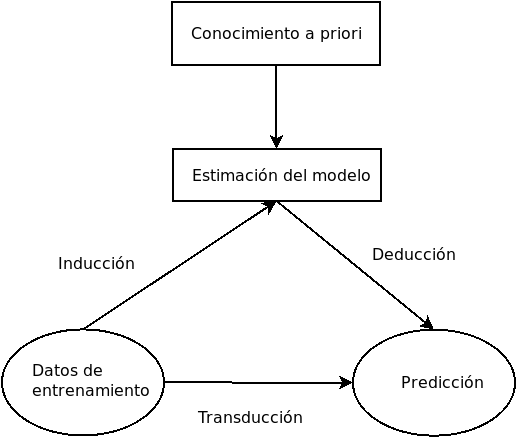
\includegraphics[scale=0.5]{imagenes/induccion_deduccion_transduccion}
	\label{ind_ded_trans}
	\caption{Tipos de inferencia y transducción \cite[p.~41]{cherkassky_learning_2007}}
\end{figure}

Podemos ver que el conocimiento a priori que tenemos del problema se manifiesta una vez se crea el modelo general, de forma que se emplearía en el paso de la inducción. Ya hemos hablado previamente del conocimiento a priori y cómo incorporarlo al modelo, pero por concretar un poco más podemos añadirlo básicamente de dos formas:

\begin{itemize}
	\item Escogiendo un conjunto de funciones para aproximar la salida del sistema
	\item Añadiendo restricciones o penalizaciones adicionales a dicho conjunto de funciones.
\end{itemize}

En resumen, para poder crear la generalización del modelo de forma única necesitamos:

\begin{enumerate}
	\item Un conjunto de funciones para aproximar la salida.
	\item Conocimiento a priori.
	\item Un principio inductivo, que no es más que una indicación de cómo emplear los datos para llegar a la generalización del modelo.
	\item Un método de aprendizaje, es decir, una implementación del principio inductivo.
\end{enumerate}

En secciones posteriores revisaremos algunos de los principios inductivos más usados pero es importante reseñar la diferencia entre principio inductivo y método de aprendizaje. Para un mismo principio inductivo podemos tener varios métodos de aprendizaje, pues podemos escoger diferentes formas de llevarlo a la práctica. Por ejemplo, uno de los principios inductivos más empleados es el ERM o Empirical Risk Minimization, es decir, minimización del error empírico. Podríamos pensar en diferentes formas de utilizar este principio, por ejemplo sólo avanzamos en la creación del modelo si a cada paso que demos minimizamos el error, o por ejemplo vamos avanzando varios modelos a la vez hasta obtener un número de modelos finales de entre los cuales escogeremos aquel que mejor minimice dicho error.

\subsection{Principios inductivos}

Una vez introducido el concepto como hemos hecho en la sección anterior vamos a hacer un breve repaso de los principios más usados y en qué consiste cada uno de ellos.

\subsubsection{Penalización o Regularización}

Imaginemos que tenemos una clase de funciones muy flexible, esto es con un gran número de parámetros libres $f(x,\omega)$ con $\omega \in \Omega$. Vamos a partir de la base del ERM, es decir, minimizar el error empírico. La penalización lo que va a hacer es añadir un factor a la función a minimizar:

$$R_{pen}(\omega) = R_{emp}(\omega) + \lambda \phi [f(x,\omega)]$$

Donde $R_{emp}(\omega)$ es el error empírico con los parámetros $\omega$ y $\phi [f(x,\omega)]$ es un funcional no negativo asociado a cada estimación $f(x,\omega)$. El parámetro $\lambda >0$ es un escalar que controla el peso de la penalización.

El funcional $\phi [f(x,\omega)]$ puede medir lo que creamos conveniente que debemos añadir, es decir, aquí podemos añadir a la minimización algún tipo de medida que nos diga cómo de bien funciona el ajuste de los datos y cómo de bien funciona la información a priori que hemos incluido en el modelo. Pensemos por ejemplo que $\lambda$ fuera un parámetro con un valor muy alto. En este caso la penalización por un mal ajuste de los datos no sería de gran importancia pues lo más conveniente sería minimizar el valor del funcional para no obtener una gran penalización. De esta forma podemos ajustar y dar un poco más de información al error empírico. Por ejemplo, en función del problema, es posible medir la complejidad de la solución mediante el funcional $\phi$ y de esta forma no sólo vamos a obtener una función que ajuste bien los datos, si no que también mantenga una cierta simplicidad para evitar por ejemplo el sobreajuste.

\subsubsection{Reglas de parada anticipada}

Pensemos en un método que vaya aprendiendo de los datos de forma iterativa intentando a cada iteración reducir el error cometido, por ejemplo el ERM. Los métodos o reglas de parada anticipada pueden verse como penalizaciones sobre el algoritmo conforme se va ejecutando. Las reglas de parada anticipada, como su nombre indica lo que prevén es la parada del algoritmo antes de obtener su objetivo teórico. Por ejemplo un algoritmo intenta que el error sea menor que $10^{-6}$ pero para reducirlo desde $10^{-4}$ hasta $10^{-5}$ está consumiendo millones de iteraciones. Si queremos que el tiempo de cómputo penalice lo que podemos hacer es fijar por ejemplo un número máximo de iteraciones que detenga el método aunque no se haya alcanzado esa barrera de error que se preveía.

\subsubsection{Minimización del riesgo estructural o SRM}

Para entender esta filosofía nos ponemos en la situación de que ya sabemos la clase de funciones con la que vamos a aproximar la salida del sistema, por ejemplo hemos escogido la clase de funciones polinómicas. Bajo esta clase de funciones podemos ordenar las funciones por complejidad, entendiendo por complejidad el número de parámetros de la función. Por ejemplo los polinomios de grado $m$ son de menor complejidad que los de grado $m+1$. De esta forma podemos pensar en una estructura de la clase de funciones de la forma:

$$S_0 \subset S_1 \subset S_2 \subset \cdots$$

Este parámetro de complejidad también puede ser un principio a minimizar para intentar conseguir una solución adecuada pero también simple. La generalización de la medida de complejidad para las clases de funciones es la conocida como dimensión VC o dimensión de Vapnik-Chervonenkis.

\subsubsection{Inferencia Bayesiana}

Este principio inductivo se utiliza en el problema de estimación de la función de densidad. El principio es utilizar la conocida fórmula de Bayes para hacer una estimación de la función de densidad empleando el conocimiento a priori que disponemos del problema. La forma en la que se emplea esta fórmula es de la siguiente:

$$P[modelo | datos] = \frac{P[datos | modelo] \cdot P[modelo]}{P[datos]}$$

, donde $P[modelo]$ es la probabilidad a priori, $P[datos]$ es la probabilidad de los datos de entrenamiento y $P[datos | modelo]$ es la probabilidad de que los datos estén generados por el modelo.

\subsubsection{Descripción de mínima longitud}

La idea de este principio es la minimización de la longitud que se necesita emplear para describir un modelo y la correspondiente salida. Llamamos l a la longitud total:

$$l = L(modelo) + L(datos | modelo).$$

Esta medida puede ser vista como una medida de complejidad conjunta de todo el modelo.

\section{Regularización}

Por la importancia de este principio inductivo vamos a desarrollarlo un poco más, junto con el concepto de penalización, la selección de los modelos y la relación entre sesgo y varianza. Este último es un concepto muy relevante en cuanto al aprendizaje y que en nuestro caso, al no poseer la clasificación real tendremos que tenerlo en cuenta.

\subsection{Problema de la alta dimensionalidad}

Sabemos que cuando estamos ante un problema de aprendizaje nuestro objetivo es conseguir estimar una función con un número finito de instancias de una muestra ya con la salida. Al tener un número finito de elementos en la muestra ya sabemos que no podemos garantizar que la respuesta sea la óptima o correcta, pero además debemos pensar que a mayor regularidad del conjunto de funciones empleado debemos tener una densidad suficiente de puntos para compensar dicha regularidad. Este problema es conocido como la maldición de la dimensionalidad (curse of dimensionality). El problema es que cuanto mayor sea la dimensionalidad considerada más difícil es poder tener esa alta densidad de datos que se requieren para funciones muy regulares.

Este problema que conlleva la alta dimensionalidad proviene de la geometría de los espacio con alta dimensionalidad. A medida que incrementamos la dimensionalidad el espacio se ve cada vez con más aristas o picos. Podemos pensar en un cubo para el espacio tridimensional y a medida que aumentamos la dimensión incorporamos más aristas y vértices. Podemos resumir en 4 propiedades de los espacio con alta dimensionalidad que causan este problema:

\begin{enumerate}
	\item La densidad disminuye exponencialmente al aumentar el número de dimensiones. Supongamos que tenemos una muestra de $n$ puntos en $\mathbb{R}$. Para poder tener la misma densidad en un espacio $d$-dimensional $\mathbb{R}^d$ necesitamos $n^d$ puntos.
	\item Cuanto mayor dimensionalidad tenga el conjunto de datos mayor lado se necesita para que un hipercubo contenga el mismo porcentaje del conjunto que con una menor dimensionalidad. Imaginemos que tenemos un conjunto $d$-dimensional en el que tenemos la muestra dentro de un hipercubo unidad. Si quisiéramos abarcar un porcentaje $p\in [0,1]$ necesitaríamos un cubo de lado $e_d (p) = p^{\frac{1}{d}}$. Como se puede observar a mayor dimensionalidad y $p$ constante el lado es cada vez mayor. Esta idea es fácilmente entendible si observamos la siguiente figura:
	
	\begin{figure}[H]
		\centering
		\label{radio_alta_dimensionalidad}
		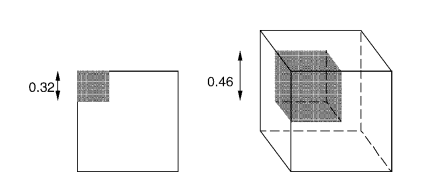
\includegraphics[scale=0.6]{imagenes/radio_alta_dimensionalidad}
		\caption{Para 2 dimensiones necesitamos menor lado que para 3 dimensiones. \cite[p.~64]{cherkassky_learning_2007}}
	\end{figure}
	\item Casi todo punto está más cerca de un borde que de otro punto. Pensemos en un conjunto de datos con $n$ puntos distribuidos de forma uniforme en una bola $d$-dimensional de radio unidad. Para este conjunto de datos, según Hastie \cite{hastie_t._elements_nodate}, la distancia media entre el centro de la distribución y los puntos más cercanos a dicho centro se mide bajo la fórmula:
	
	$$D(d,n) = (1-\frac{1}{2}^{1/n})^{1/d}$$
	
	Si en esta fórmula tomamos por ejemplo $n=200$ y $d=10$ el resultado es $D(10,200) \approx 0.57$. Esto significa que los puntos más cercanos al centro de la distribución están más cerca de los bordes que del centro.
	\item Casi todo punto es una anomalía sobre su propia proyección. Si pensamos de nuevo en la idea de los vértices y aristas en espacio de alta dimensionalidad y pensamos en que, según el punto anterior, cada vez que aumenta la dimensionalidad los puntos están más cerca de los bordes entonces no es extraño pensar que los puntos a medida que aumenta la dimensionalidad están más distantes del resto de puntos. Esto intuitivamente (ya que aún no hemos visto la definición formal de anomalía) nos guía a pensar que vistos los puntos en sus propios entornos éstos serán anomalías comparados con el resto.
	
	\begin{figure}[H]
		\centering
		\label{espacio_alta_dimension}
		
\includegraphics[scale=0.6]{imagenes/espacio_alta_dimension}
		\caption{Forma conceptual de un espacio de alta dimensionalidad.\cite[p.~64]{cherkassky_learning_2007}}
	\end{figure}

	Conceptualmente podemos imaginarlo con esta forma de picos, con lo que si tenemos los datos apiñados en dichos picos o extremos el resto de datos que estén en picos diferentes distan tanto del que estamos considerando que no podemos afirmar que tengan ninguna relación entre sí.
\end{enumerate}

Estos puntos hemos de recordar que van referidos al conjunto de datos y no a las funciones que estamos considerando para representar la salida del sistema. Si estamos considerando la complejidad de las funciones la dimensionalidad no es una buena medida. Sabemos de la existencia de teoremas de aproximación de funciones como por ejemplo el Teorema de Superposición de Kolmogorov-Arnold.

\begin{teorema}[Teorema de Superposición de Kolmogorov-Arnold]
	Sea $f$ una función continua de varias variables $f:X_1 \times ... \times X_n \rightarrow \mathbb{R}$, entonces existen funciones $\Phi_q : \mathbb{R}\rightarrow \mathbb{R}$ y $\phi_{q,p} : X_p \rightarrow [0,1]$ tales que $f$ se puede expresar como:
	
	$$f(x) = f(x_1, ..., x_n) = \sum_{q=0}^{2n}\Phi_q ( \sum_{p=1}^{n}\phi_{q,p}(x_p))$$
\end{teorema}

Este Teorema argumenta perfectamente que la complejidad que le damos a los datos por tener una alta dimensionalidad no es transferible a las funciones pues podemos expresar funciones de varias variables como combinación de funciones de una sola variables. En otras palabras no podemos argumentar que la complejidad de funciones univariantes sea mayor o menor que la de funciones multivariantes.

\subsection{Aproximación de funciones}

Como ya hemos dicho en la introducción queremos aproximar una función salida del sistema dentro de una familia de funciones. Este campo no es nuevo, tenemos como herramientas una serie de Teoremas relacionados con la aproximación de funciones como el Teorema de Kolmogorov enunciado anteriormente o el Teorema de aproximación de Weierstrass.

La versión más simple del Teorema de Weierstrass es la de funciones reales definidas en intervalos cerrados, veamos un repaso de estos Teoremas para hacer un esquema de la aproximación de funciones.

\begin{teorema}[Teorema de aproximación de Weierstrass]
	Supongamos que $f:[a,b] \rightarrow \mathbb{R}$ es una función continua. Entonces $\forall \epsilon >0$, $\exists p$ un polinomio tal que $\forall x\in [a,b]$ tenemos que $|f(x)-p(x)|<\epsilon$.
\end{teorema}

En otras palabras, podemos aproximar las funciones continuas reales definidas en un intervalo cerrado con el error que queramos en un punto mediante polinomios. Además tenemos versiones más generales aún como el Teorema de Stone-Weierstrass para funciones reales, para espacios localmente compactos y para el espacio de los complejos.

Estas aproximaciones son más sencillas en términos de la complejidad de la clase de funciones, pero tenemos aproximaciones muy famosas, como por ejemplo la serie de Fourier.

\begin{definicion}[Serie de Fourier]
	Si tenemos una función $f:\mathbb{R} \rightarrow \mathbb{R}$ integrable en el intervalo $[t_0 - \frac{T}{2}, t_0 + \frac{T}{2}]$ entonces se puede obtener el desarrollo en serie de Fourier de $f$ en dicho intervalo. Si $f$ es periódica en toda la recta real la aproximación será válida en todos los valores en los que esté definida.
	
	$$f(t) \approx \frac{a_0}{2} + \sum_{n=1}^{\infty}[a_n \cos (\frac{2n\pi}{T}t) + b_n\sin (\frac{2n\pi}{T}t)]$$
	
	Donde $a_0, a_n$ y $b_n$ son los coeficientes de la serie de Fourier que tienen la forma:
	
	$$a_0 = \frac{2}{T}\int_{-\frac{T}{2}}^{\frac{T}{2}}f(t)dt$$
	
	$$a_n = \frac{2}{T}\int_{-\frac{T}{2}}^{\frac{T}{2}}f(t) cos(\frac{2n\pi}{T}t)dt$$
	
	$$b_n = \frac{2}{T}\int_{-\frac{T}{2}}^{\frac{T}{2}}f(t) \sin (\frac{2n\pi}{T}t)dt$$
\end{definicion}

Como podemos ver hemos introducido dos conocidas formas de aproximar funciones, una con funciones polinómicas y otra con funciones trigonométricas. Vamos a dividir en dos los tipos de  aproximación que podemos tener para el problema de aprendizaje.

\begin{enumerate}
	\item Aproximaciones universales: son aquellas en las que se establece que cualquier función continua puede ser aproximada por otra función de otra clase con el error que queramos. En este grupo podríamos meter a los dos teoremas que hemos dado previamente. Dentro de este grupo podemos tener diferentes tipos de aproximaciones en función de la familia de funciones que escojamos como aproximaciones. Por ejemplo en los dos teoremas previos hemos cogido las clases de funciones polinómicas y trigonométricas pero podríamos haber tomado otras clases diferentes.
	\item Aproximaciones inexactas: son aquellas en las que no podemos tener una aproximación como las que hemos dado en los teoremas previos, si no que proveen de una aproximación de peor calidad.
\end{enumerate}

\subsection{Penalización o control de la complejidad}

Ya hemos discutido brevemente en la sección de principios inductivos la complejidad y cómo penalizarla. Vamos a ver qué elementos queremos controlar con la penalización:

\begin{enumerate}
	\item La clase de funciones con la que vamos a hacer la aproximación. Tenemos que decidir si escoger una clase tan amplia que nos aseguremos que abarque la solución seguro pero penalicemos la complejidad de la elección o queremos una clase de funciones más ajustada.
	\item Tipo de funcional de penalización. Tenemos que escoger entre los distintos tipos de penalización que queremos. Esto se reduce a escoger entre dos tipos de penalización: paramétrica y no paramétrica. La primera de ellas se basa en estudiar la suavidad del ajuste junto con el número de parámetros que requiere la aproximación mientras que la segunda intenta estudiar lo mismo, es decir la suavidad del ajuste, sin medir los parámetros de la clase de funciones. En este punto se puede incorporar el conocimiento a priori del problema.
	\item Método con el que queremos minimizar la penalización. Este apartado está relacionado con los métodos que tenemos de aprender de los datos y el objetivo será intentar hallar una forma eficiente de minimizar tanto el error de la aproximación como la propia penalización.
	\item Control de la complejidad. Como hemos dicho antes el control de la complejidad no es algo sencillo y habrá que escoger la mejor manera de medir dicha complejidad. En secciones posteriores veremos medidas de complejidad como la dimensión de Vapnik-Chervonenkis.
\end{enumerate}

Veamos brevemente la distinción que hemos hecho entre la penalización paramétrica y no paramétrica.

\subsubsection{Penalización paramétrica}

Supongamos que tenemos un conjunto de funciones $f(x,\omega)$ con $\omega \in \Omega$ donde $\Omega$ es el conjunto de parámetros de la forma $\omega = (\omega_0 , ... , \omega_m)$. Como la aproximación viene definida por el parámetros $\omega$ entonces podemos definir también la penalización asociada a dicha selección de parámetros.

Vamos a ver los ejemplos de las penalizaciones más empleadas de este tipo.

\begin{itemize}
	\item Ridge: $\phi_r (\omega_m) = \sum_{i=0}^{m}\omega_i^2$
	\item Selección de subconjunto: $\phi_s (\omega_m) = \sum_{i=0}^{m}\chi (\omega_i \neq 0)$
	\item Bridge: $\phi_p (\omega_m) = \sum_{i=0}^{m}|\omega_i|^p$
	\item Decaimiento de peso: $\phi_q (\omega_m) = \sum_{i=0}^{m}\frac{(\omega_i / q)^2}{1+(\omega_i / q)^2}$ 
\end{itemize}

\subsubsection{Penalización no paramétrica}

En primer lugar vamos a definir la transformada de Fourier de una función para poder definir el funcional de penalización. 

\begin{definicion}[Transformada de Fourier]
	Sea $f$ una función integrable Lebesgue, $f\in L(\mathbb{R})$. Se define la transformada de Fourier de $f$ como la función:
	
	$$\mathcal{F}\{f\} : \xi \rightarrow \hat{f}(\xi) := \int_{-\infty}^{\infty}f(x)e^{-2\pi i\xi x}dx$$
\end{definicion}

Recordemos brevemente las propiedades de la transformada de Fourier.

\begin{itemize}
	\item La transformada de Fourier es un operador lineal: $\mathcal{F}\{a\cdot f + b\cdot g\} = a\mathcal{F}\{f\} + b\cdot \mathcal{F}\{g\}$
	\item $\mathcal{F}\{f(at)\}(\xi) = \frac{1}{|a|}\cdot \mathcal{F}\{f\}(\frac{\xi}{a})$
	\item $\mathcal{F}\{f(t-a)\}(\xi) = e^{-\pi i\xi a}\cdot \mathcal{F}\{f\}(\xi)$
	\item $\mathcal{F}\{f\}(\xi -a) = \mathcal{F}\{e^{\pi iat}f(t)\}(\xi)$
	\item $\mathcal{F}\{f'\}(\xi) = 2\pi i\xi \mathcal{F}\{f\}(\xi)$
	\item $\mathcal{F}\{f\}'(\xi) = \mathcal{F}\{(-it)\cdot f(t)\}(\xi)$
\end{itemize}

Habiendo recordado esto podemos definir el funcional de penalización no paramétrica. Este funcional mide la suavidad del ajuste de la función gracias a que se puede medir, mediante la transformada de Fourier, la ondulación de la función. Por tanto el funcional no paramétrico que se propone es:

$$\phi [f] = \int_{\mathbb{R}^d}\frac{|\hat{f}(s)|^2}{\hat{G}(s)}ds$$

Donde $\hat{f}$ indica la transformada de Fourier de la función $f$ y $\frac{1}{\hat{G}}$ es la transformada de Fourier de una función de filtro de paso alto. Es en esta proposición de filtro donde se añade el conocimiento a priori del problema. Por ejemplo pudiera ser interesante en alguna aplicación práctica tener un funcional invariante frente a rotaciones de funciones.

\subsection{Equilibrio entre el sesgo y la varianza}

Este enfoque es muy utilizado en el estudio del error, dividiéndolo en sesgo y varianza para hacer un mejor estudio del mismo y poder enfrentar ambos con varios métodos. Este estudio del caso clásico no es válido (o al menos no del todo) para problemas no supervisados como es nuestro caso. Vamos a hacer una adaptación de esta teoría para que pueda encajar en nuestro caso de estudio.

Tenemos que tener en cuenta que no conocemos la salida real del sistema en el caso de detección de anomalías, es decir, no sabemos estimar con certeza el sesgo y la varianza y por tanto el error que cometemos. En primer lugar vamos a ver una pequeña adaptación de la notación al caso de detección de anomalías para poder hacer un estudio enfocado en nuestro problema.

Vamos a notar por $X_1 , ... , X_n$ los datos de test y $\mathcal{D}$ como conjunto de datos de entrenamiento. Además vamos a considerar que existe una función $f$ que nos da la etiqueta real de un dato, esto es, si es o no una anomalía. Por tanto podemos decir que la auténtica etiqueta de un dato es $y_i = f(X_i)$. Además nosotros estaremos usando un modelo ya escogido por nosotros para predecir la etiqueta de un dato de test, esto es $g(X_i, \mathcal{D})\approx y_i+\beta$ donde $\beta$ es un cierto error.

Una vez conocida esta notación podemos definir el error medio al cuadrado como:

$$MSE = \frac{1}{n}\sum_{i=1}^{n}\{y_i - g(X_i, \mathcal{D})\}^2$$

Y podemos definir también el valor esperado del error medio al cuadrado como:

$$E[MSE] = \frac{1}{n} \sum_{i=1}^{n}E[\{y_i - g(X_i, \mathcal{D})\}^2]$$

Una vez definido el $MSE$ esperado podemos desarrollar un poco el cálculo para poder obtener el error y la varianza que esperamos.

En primer lugar podemos escribirlo como:

$$E[MSE] = \frac{1}{n}\sum_{i=1}^{n}E[\{ (y_i-f(X_i)) + (f(X_i) - g(X_i,\mathcal{D})) \}^2]$$

Aquí solo hemos restado y sumado $f(X_i)$, ahora si recordamos que $y_i = f(X_i)$ entonces podemos igualar el primero de los paréntesis a $0$ y por tanto nos queda:

$$E[MSE] = \frac{1}{n}\sum_{i=1}^{n}E[\{ f(X_i) - g(X_i, \mathcal{D}) \}^2]$$

Si seguimos descomponiendo podemos sumar y restar $E[g(X_i, \mathcal{D})]$ con lo que nos quedaría:

$$E[MSE] = \frac{1}{n}\sum_{i=1}^{n}E[\{ f(X_i) - E[g(X_i, \mathcal{D})] \}^2]$$

$$ + \frac{2}{n}\sum_{i=1}^{n}\{ f(X_i) - E[g(X_i, \mathcal{D})] \}\cdot \{ E[g(X_i, \mathcal{D})] - E[g(X_i, \mathcal{D})] \}$$

$$ + \frac{1}{n}E[\{ E[g(X_i, \mathcal{D}) - g(X_i, \mathcal{D})] \}^2]$$

Como es claro, el segundo término da cero por lo que nos queda al final:

$$E[MSE] = \frac{1}{n} \sum_{i=1}^{n}E[\{ f(X_i) - E[g(X_i, \mathcal{D})] \}^2] + \frac{1}{n}\sum_{i=1}^{n}E[\{ E[g(X_i, \mathcal{D})] - g(X_i, \mathcal{D}) \}^2]$$

$$=\frac{1}{n}\sum_{i=1}^{n}\{ f(X_i) - E[g(X_i, \mathcal{D})] \}^2 + \frac{1}{n}\sum_{i=1}^{n}E[\{ E[g(X_i, \mathcal{D})] - g(X_i, \mathcal{D}) \}^2]$$

Si reconocemos cada uno de los términos, en primer lugar el primero de ellos es el sesgo al cuadrado y el segundo la varianza, por lo que finalmente lo que hemos obtenido es:

$$E[MSE] = sesgo^2 + varianza$$

El dilema que se nos plantea es el siguiente: si tomamos modelos con un bajo sesgo en la estimación de los parámetros entonces tendremos una alta varianza y viceversa. Esto significa que no podemos con el conocimiento del que disponemos disminuir tanto el sesgo como la varianza a la vez. Es esta propiedad la que se conoce como la compensación entre sesgo y varianza.

\section{Teoría estadística del aprendizaje}

En esta sección vamos a hacer un repaso por la teoría del aprendizaje, en concreto la teoría desarrollada por Vapnik-Chervonenkis. Esta teoría se basa o tiene como pilares cuatro puntos:

\begin{enumerate}
	\item Condiciones para la consistencia del principio ERM o minimización del error empírico.
	\item Cotas en la capacidad de generalización de las máquinas de aprendizaje.
	\item Principios de inferencia sobre muestras finitas.
	\item Métodos constructivos para implementar los principios inductivos ya expuestos.
\end{enumerate}

Durante el desarrollo de esta sección haremos un repaso de estos cuatro puntos para dar el broche final a esta sección y poder realizar la primera de las definiciones de anomalía.

\subsection{Condiciones para la convergencia y consistencia del ERM}

En el problema de aprendizaje disponemos de una muestra en la que tenemos los propios datos de entrada y la salida del sistema. Denotemos a estos elementos por $z=(x,y)$ donde $x$ son los datos de entrada e $y$ la salida del sistema. Por tanto la muestra que se nos da es un conjunto $Z_n = \{ z_1 , ... , z_n \}$. Estos datos están generados como ya sabemos mediante una función de densidad desconocida $p(z)$. Sobre este esquema tenemos una serie de funciones de pérdida y un funcional de pérdida. El objetivo es encontrar dicha función de pérdida $Q(z,\omega )$ que minimice dicho funcional:

$$R(\omega) = \int Q(z,\omega) p(z)dz$$

Por tanto si tenemos la función de pérdida podemos definir el error empírico como:

$$R_{emp}(\omega) = \sum_{i=1}^{n}Q(z_i, \omega)$$

Donde $\omega$ son los parámetros escogidos para el modelo.

Para poder estudiar la consistencia del ERM primero debemos definir formalmente dicha propiedad. Denotamos por $R_{emp}(\omega_n^*)$ el valor del error empírico con la función de pérdida $Q(z,\omega_n^*)$ que minimiza el error empírico para el conjunto de entrenamiento $Z_n$. Denotemos además por $R(\omega_n^*)$ el verdadero valor (desconocido) del error para la función de pérdida. Como se puede ver estos valores dependen del tamaño del conjunto de entrenamiento $n$, podemos por tanto estudiar cómo se comportan estos errores cuando aumentamos el tamaño del conjunto de entrenamiento. Es aquí donde entra la definición de consistencia del ERM. Decimos que es consistente si la sucesión de errores reales y empíricos convergen en probabilidad al mismo límite $R(\omega_0) = \min_{\omega} R(\omega)$. Es decir:

$$R(\omega_n^*) \rightarrow R(\omega_0) \ cuando \ n\rightarrow \infty$$
$$R_{emp}(\omega_n^*) \rightarrow R(\omega_0) \ cuando \ n\rightarrow \infty$$

Para poder asegurar esta propiedad sobre el ERM tenemos el conocido como Teorema Clave de la Teoría del Aprendizaje de Vapnik y Chervonenkis.

\begin{teorema}[Teorema Clave de la Teoría del Aprendizaje]
	Para funciones de pérdida acotadas el principio inductivo de minimización del error empírico es consistente sí y sólo si el error empírico converge uniformemente al valor real del error en el siguiente sentido:
	
	$$\lim\limits_{n\rightarrow \infty} P[\sup_{\omega}|R(\omega) - R_{emp}(\omega)|>\epsilon] = 0 \ , \ \forall \epsilon >0$$
\end{teorema}

Cabe recalcar que estas condiciones de consistencia dependen de las propiedades de la clase de funciones elegida. No podemos pretender escoger como clase de aproximación una muy general y seguir manteniendo las condiciones de consistencia del ERM. Aún así el teorema nos está dando condiciones generales para la consistencia del ERM pero son abstractas y no fácilmente aplicables en la práctica. Para ello vamos a estudiar las condiciones de convergencia de ERM que sí serán aplicables en la implementación de algoritmos.

Vamos ahora a particularizar el estudio en el caso de clasificación binaria por ser la materia de estudio que nos ocupa, pues al final tendremos que clasificar instancias en anómalas o no anómalas. Ahora las funciones de pérdida $Q(z,\omega)$ son funciones de pérdida indicadoras. Vamos a notar por $N(Z_n)$ el número de dicotomías que se pueden tener con la clase de funciones elegidas. Esto es el número de formas de clasificar los datos en las dos clases existentes.

Una vez actualizada nuestra notación podemos definir la entropía aleatoria como $H(Z_n) = \ln N(Z_n)$. Esta cantidad es una variable aleatoria dependiente de los valores de entrenamiento $Z_n$, podemos definir ahora la entropía de Vapnik-Chervonenkis como el valor medio o esperado de la entropía aleatoria:

$$H(n) = E[\ln N(Z_n)]$$

Esta medida es una cuantificación de la diversidad del conjunto de funciones indicadoras que nos pueden separar los datos en ambas clases.

Por último vamos a definir la función de crecimiento que nos va a permitir hacer cotas y llegar a la condición necesaria y suficiente para la convergencia del ERM. Definimos la función de crecimiento como:

$$G(n) = \ln \max_{Z_n} N(Z_n)$$

Donde aquí estamos notando el máximo número de dicotomías sobre todas las posibles muestras existentes de tamaño $n$. Es más, como el máximo número de formas de dividir un conjunto de tamaño $n$ en dos clases es $2^n$ entonces podemos afirmar que $G(n)\leq n\ln (2)$.

Por último y para completar la cadena de desigualdades que buscamos vamos a definir la entropía reforzada de Vapnik-Chervonenkis:

$$H_{ann}(n) = \ln (E[N(Z_n)])$$

Haciendo uso de la conocida desigualdad de Jensen,

$$\sum_{i=1}^{n}a_i \ln (x_i) \leq \ln (\sum_{i=1}^{n}a_i x_i)$$,

 podemos ver claramente que $H(n)\leq H_{ann}(n)$. Por tanto obtenemos la cadena de desigualdades:

$$H(n)\leq H_{ann}(n) \leq G(n) \leq n\ln (2)$$

La condición necesaria y suficiente de Vapnik-Chervonenkis para la convergencia del ERM que hallaron fue que:

$$\lim\limits_{n\rightarrow \infty} \frac{H(n)}{n} = 0$$

Pero esta condición no asegura una convergencia rápida asintóticamente al error real. Se dice que el ratio de convergencia es rápido asintóticamente en la Teoría de Vapkin-Chervonenkis si:

$$\forall n>n_0 \ P(R(\omega) - R(\omega^*)<\epsilon) = e^{-cn\epsilon^2} \ con \ c>0$$

Para poder cumplir esta condición se dio la condición suficiente para la convergencia rápida:

$$\lim\limits_{n\rightarrow \infty} \frac{H_{ann}(n)}{n} = 0$$

Estas condiciones son dependientes de la distribución de los datos $Z_n$ como es claro al depender de la esperanza de una variable aleatoria dependiente de $Z_n$. Es por tanto que esta condición no es del todo general. Para solventar esto se tiene la consistencia y convergencia del ERM con la condición necesaria y suficiente de que:

$$\lim\limits_{n\rightarrow \infty}\frac{G(n)}{n}$$

Por tanto este estudio nos ha dado las condiciones de convergencia y consistencia del ERM.

\subsection{Función de crecimiento y dimensión de Vapnik-Chervonenkis}

El objetivo que perseguimos es obtener cotas para la capacidad de generalización de las máquinas de aprendizaje. Para dar el primer paso según hemos visto necesitamos una forma de evaluar la función de crecimiento vista en el apartado anterior, cosa que no es sencilla de llevar a la práctica.

Para continuar avanzando en este camino lo primero que vamos a presentar es el concepto de dimensión de Vapnik-Chervonenkis o dimensión VC. Cuando discutimos cómo medir la complejidad de un modelo ya hablamos de que la dimensión VC podría ser una buena herramienta para este fin, la introducimos a continuación.

Vapnik y Chervonenkis probaron que la función de crecimiento estaba acotada por una función logarítmica en función del tamaño de la muestra. El punto en el que se tiene $n=h$ donde $h$ es un valor fijo se tiene que el crecimiento de la función de crecimiento empieza a ralentizarse, esta es la conocida como dimensión VC. Si $h$ es un número finito entonces tenemos que la función de crecimiento no va a crecer de forma lineal para muestras de tamaño grande y de hecho se tiene la cota:

$$G(n)\leq h(1+\ln (\frac{n}{h}))$$

La dimensión de Vapnik-Chervonenkis es intrínseca a la elección del conjunto de funciones y además nos da condiciones sobre la convergencia rápida del ERM. Ya hemos visto antes que la cota más grande de la función de crecimiento es:

$$G(n)\leq n\ln (2)$$

Si comparamos las dos cotas en función de n tenemos la siguiente gráfica:

\begin{figure}[H]
	\centering
	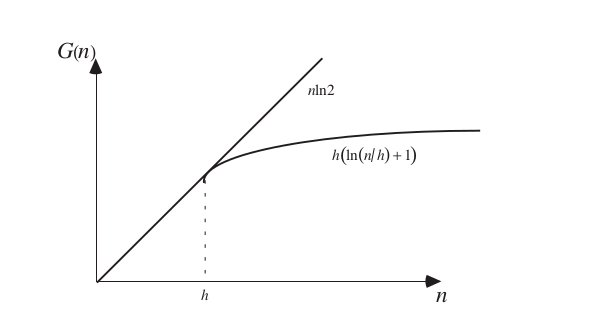
\includegraphics[scale=0.6]{imagenes/funcion_crecimiento_dimension_vc}
	\label{funcion_crecimiento_dimension_vc}
	\caption{Comportamiento de la función de crecimiento \cite[p.~107]{cherkassky_learning_2007}}
\end{figure}

Como podemos ver el comportamiento una vez que el tamaño de la muestra alcanza la dimensión VC converge de forma mucho más rápida.

Hasta ahora no hemos definido formalmente la dimensión VC pero hemos dado una característica de la misma que nos garantiza una buena convergencia. Decimos que un conjunto de funciones indicadoras tiene dimensión VC $h$ si existe una muestra de puntos de tamaño $h$ que puede ser dividida pero no existe una muestra de tamaño $h+1$ que cumpla dicha condición. Es decir, podemos decir que la dimensión VC es la máxima dimensión para la que existe una solución óptima a nuestro problema de dividir el conjunto de datos entre datos anómalos y normales.

Veamos esto con un ejemplo gráfico:

\begin{figure}[H]
	\centering
	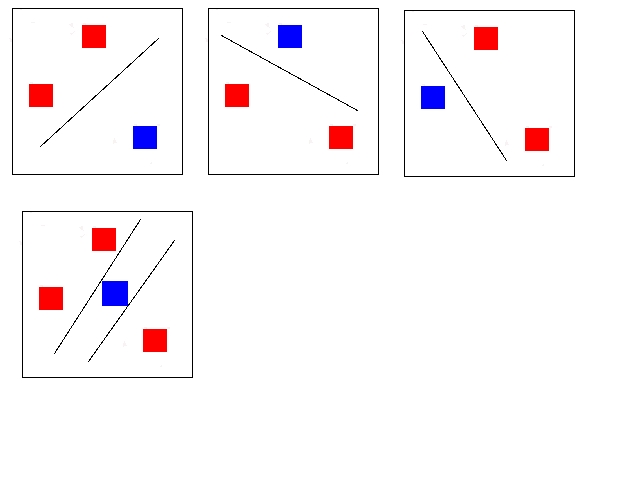
\includegraphics[scale=0.35]{imagenes/dimension_vc}
	\label{dimension_vc}
	\caption{Ejemplo de cálculo de dimensión VC \href{https://commons.wikimedia.org/wiki/File:Vc_linear.jpg}{Wikimedia}}
\end{figure}

Como podemos ver si estamos considerando funciones lineales para aproximar podemos dividir todas las posibilidades con tamaño de muestra 3, pero no con tamaño de muestra 4 por lo que en este caso concreto la dimensión VC será 3.

Ahora podemos volver a la cadena de desigualdades que hemos visto en la sección anterior y actualizarla con la nueva mejor cota que hemos desarrollado con la dimensión VC:

$$H(n)\leq H_{ann}(n) \leq G(n) \leq h(1+\ln (\frac{n}{h}))$$

La definición que hemos dado es para funciones indicadoras pero no para funciones reales en general, vamos a generalizar por tanto la definición de la dimensión de Vapnik-Chervonenkis para el caso de funciones reales.

Consideramos como hemos hecho anteriormente funciones de pérdida del tipo $Q(z,\omega)$ pero acotadas superior e inferiormente por constantes:

$$A\leq Q(z,\omega) \leq B$$

Para este caso podemos pensar en una función indicadora que nos diga si $Q(z,\omega)$ está por encima o por debajo de un cierto valor $\beta$ con $A\leq \beta \leq B$. Podemos por tanto generalizar la dimensión VC para el caso de funciones de pérdida reales como la dimensión VC de este tipo de funciones indicadoras dependientes del parámetro $\beta$.

\subsection{Límites de la generalización}

Venimos de discutir las propiedades de convergencia y consistencia del principio inductivo ERM. Ahora bajo este principio vamos a intentar ir un paso mas allá en la generalización e intentar responder a las siguientes dos preguntas:

\begin{enumerate}
	\item ¿Cómo de cerca están el error real $R(\omega^*)$ y el mínimo error empírico $R_{emp}(\omega^*)$?
	\item ¿Cómo de cerca están el error real $R(\omega^*)$ y el mínimo error posible $R(\omega_0) = \min_{\omega} R(\omega)$?
\end{enumerate}

Estas preguntas las vamos a resolver en el marco que hemos introducido, con todos los conceptos anteriores de la teoría de Vapnik-Chervonenkis en el caso del problema de clasificación binaria que es el que más se ajusta a nuestro problema.

Según Vapnik-Chervonekis se puede acotar el error real cometido por el error empírico con una probabilidad de al menos $1-\eta$ usando el principio inductivo ERM. La cota que hallaron es la siguiente:

$$R(\omega) \leq R_{emp}( \omega) + \frac{\epsilon}{2} \biggl( 1+\sqrt{1+\frac{4\cdot R_{emp}(\omega)}{\epsilon}} \biggl)$$

donde:

$$\epsilon = a_1 \cdot \frac{h(\ln (\frac{a_2 n}{h})+1) - \ln (\frac{\eta}{4})}{n}$$

cuando el conjunto de funciones de pérdida $Q(z, \omega)$ contiene un número infinito de elementos, en caso contrario:

$$\epsilon = 2\frac{\ln (N) - \ln (\eta)}{n}$$

y los valores $a_1 , a_2$ son constantes sobre los que se exigen condiciones.

Para empezar según la demostración de Vapnik, los valores $a_1$ y $a_2$ deben estar en los rangos $0<a_1 \leq 4$ y $0<a_2 \leq 2$ siendo la pareja de valores $a_1 = 4$ y $a_2 = 2$ la correspondiente al peor de los casos, dando en como resultado el siguiente valor de $\epsilon$:

$$\epsilon = 4\frac{h(\ln (\frac{2n}{h})) - \ln (\frac{\eta}{4})}{n}$$

Con esta desigualdad estamos dando la cota de cómo se comporta el error real con respecto al error empírico. Podemos ver que, en el mejor de los casos el error real y el error empírico se van a diferenciar en al menos $\frac{\epsilon}{2}$.

Además, para resolver la segunda de las preguntas la teoría de Vapnik-Chervonenkis nos da la siguiente cota con probabilidad al menos $1-2\eta$:

$$R(\omega_n^*)-\min_{\omega} R(\omega) \leq \sqrt{\frac{-\ln (\eta)}{2n}} + \frac{\epsilon}{2} \left( 1+\sqrt{1+\frac{4}{\epsilon}} \right)$$

En este caso podemos ver que la cota es aún mayor que en el caso anterior, teniéndose tanto en esta cota como en la anterior que a mayor nivel de confianza (menor valor de $\eta$) mayor es la cota y por tanto menos información tenemos. Es decir, no podemos conocer una buena cota con un nivel de confianza alto. Este hecho no debería de sorprendernos pues seguimos trabajando con un número finito de datos y ya sabemos que no podemos obtener una aproximación todo lo buena que queramos con un número finito de datos de entrenamiento.

Este hecho también se refleja en los valores analíticos que hemos dado. Pensemos en un escenario con $\eta \rightarrow 0$, es decir un alto nivel de confianza. Entonces si miramos la expresión de $\epsilon$ podemos observar que $-\ln (\frac{\eta}{4})\rightarrow \infty$ y por tanto $\epsilon \rightarrow \infty$ con lo que la cota no nos aportaría ninguna información en ninguno de los dos casos.

Por otro lado si lo que crece es el tamaño de la muestra, es decir, $n\rightarrow \infty$, estamos aumentando el conocimiento que tenemos sobre el problema y por tanto lo razonable sería que ambas cotas tendieran al valor óptimo. En efecto si observamos el valor de $\epsilon$ cuando $n\rightarrow \infty$ vemos que tiende a $0$ por lo que el error empírico y real están muy cerca y de igual forma el error real y el mínimo error posible. Por tanto podemos decir que nuestro nivel de certeza depende del tamaño de la muestra. Este hecho fue visto por Vapnik en su teoría y propuso como valor aproximado de la confianza de la desigualdad aquel que lleva asociado el valor:

$$\eta = \min (\frac{4}{\sqrt{n}},1)$$

\subsection{Principio de minimización del error estructural (SRM)}

Hemos visto una construcción en base al principio inductivo ERM y hemos razonado que funciona bien para casos en los que la proporción $\frac{n}{h}$, es decir la proporción del tamaño de la muestra y la dimensión VC, es grande. En este caso quiere decir que tenemos muchos datos comparado con la dimensión VC y por tanto $\epsilon \approx 0$. Por contra cuando tenemos que $\frac{n}{h}$ es pequeño no tenemos mucha información de la cota. Por tanto, al estar el número de datos fijo por el problema, tenemos que buscar un conjunto de funciones para aproximar la salida del sistema que nos den una dimensión VC controlable para hacerla más o menos grande.

El principio inductivo que pretende plasmar esta idea es el principio de minimización del error estructural o SRM. Bajo este principio se le otorga a la clase de funciones de pérdida de una estructura, es decir, tenemos subconjuntos de la forma $S_k = \{ Q(z,\omega), \ \omega \in \Omega_k \}$ de forma que:

$$S_1 \subset S_2 \subset ... \subset S_k \subset ...$$

donde cada subconjunto de funciones de pérdida tiene asociada una dimensión VC $h_k$ teniéndose el orden:

$$h_1 \leq h_2 \leq ... \leq h_k \leq ...$$

Al igual que en el Teorema clave de la Teoría del Aprendizaje de Vapnik-Chervonenkis se exigía que las funciones de pérdida estuvieran acotadas en este caso vamos a pedir que las funciones contenidas en cada uno de los $S_k$ o bien estén acotadas o si no que cumplan que:

$$\sup_{\omega \in \Omega_k} \frac{(\int Q^p (z,\omega)dp(z))^{\frac{1}{p}}}{\int Q(z,\omega)dp(z)}\leq \tau_k , \ p>2$$

para alguna pareja $(p,\tau_k)$.

En cuanto a la definición del SRM hay dos estrategias prácticas que se llevan a cabo para su implementación que son:

\begin{enumerate}
	\item Mantener la dimensión VC fija y minimizar el error empírico.
	\item Mantener el error empírico constante y pequeño y minimizar la dimensión VC.
\end{enumerate}

Estas implementaciones realmente quedan muy libres en la práctica y se proponen por tanto diferentes estructuras de minimización del error empírico y la dimensión VC que se saben que funcionan bien.

Por tanto este principio no se basa meramente en el buen ajuste de los datos, si no que además pretende hacer una minimización de la complejidad del modelo propuesto.

\subsection{Aproximaciones de la dimensión VC}

Como hemos estado viendo las cotas que hemos expuesto y desarrollado dependen en mayor o menor medida de la dimensión VC. Como es lógico este valor no es fácil de calcular, y de hecho sólo se sabe para unos cuantos conjuntos de funciones de aproximación. Vapnik propuso una método para poder estimar este valor y así poder obtener unas cotas aproximadas.

El procedimiento propuesto por Vapnik consiste en, dadas dos muestras $Z_n^1 , Z_n^2$ de tamaño $n$ de pares $z_i = (x,y)$ de datos de entrada y salida del sistema vamos a medir el error empírico con nuestro modelo que cometemos observando la máxima desviación de los ratios de error de estas dos muestras independientes, es decir:

$$\xi (n) = \max_{\omega} (|Error(Z_n^1) - Error(Z_n^2|)$$

donde $Error(Z_n^i)$ es la tasa de error empírico cometido por el modelo. De acuerdo con la teoría desarrollada por Vapnik-Chervonenkis tenemos que $\xi (n)$ está acotada:

$$\xi (n) \leq \Phi (\frac{n}{h})$$

donde $h$ es la dimensión VC y:

\[ \Phi (\tau) = 
\begin{cases}
1 & si \ \tau <0.5 \\
a\frac{\ln (2\tau) + 1}{\tau - k} \bigg( \sqrt{1+\frac{b (\tau - k)}{\ln (2\tau) + 1}} + 1 \bigg) & en \ otro \ caso
\end{cases}
\]

donde $\tau = \frac{n}{h}$ y las constantes $a = 0.16$ y $b = 1.2$ son constantes estimadas empíricamente por Vapnik y $k = 0.14928$ tomada así para que $\Phi (0.5) = 1$ de forma que la cota sea muy ajustada.

Por tanto describió con esto el siguiente esquema de obtención de la aproximación de la dimensión VC:

\begin{enumerate}
	\item Generamos una muestra de tamaño $2n$ etiquetada $z_{2n}$
	\item Dividimos la muestra en dos del mismo tamaño $Z_n^1$ y $Z_n^2$
	\item Invertir las etiquetas de $Z_n^2$
	\item Mezclar los dos conjuntos de nuevo y entrenar el modelo
	\item Separar el conjunto en dos de nuevo e invertir las etiquetas del segundo, volver a mezclarlos y entrenar de nuevo el modelo
	\item Medir  la diferencia de los errores $\xi (n) = |Error(Z_n^1) - Error(Z_n^2)|$
\end{enumerate}

Como hemos dicho antes la desigualdad $\xi (n) \leq \Phi (\frac{n}{h})$ es muy ajustada y por tanto, podemos obtener la aproximación de $h$ como:

$$h^* = arg \min_{h} [\xi (n) - \Phi (\frac{n}{h})]$$

Es decir, el valor que haga dicha diferencia menor, es decir que más acerque los valores $\xi (n)$ y $\Phi (\frac{n}{h})$.

\subsection{Perspectiva}

Tras este desarrollo teórico hemos dado un marco sobre el cuál podremos cimentar el resto del trabajo y modelos empleados. Con este capítulo hemos hecho un repaso por toda la teoría básica de Machine Learning y la teoría desarrollada por Vapnik y Chervonenkis.

El siguiente paso que debemos de dar es una breve introducción de estadística multivariante que nos permita introducir nociones de probabilidad para definir las anomalías desde un punto de vista algo más formal. Tras esto, debemos introducir nociones sobre el Aprendizaje Profundo o Deep Learning desde un punto de vista teórico para poder juntar todo esto en la sección práctica de este trabajo.
%
\part{Introducción de Estadística Multivariante y concepto probabilístico de anomalía}
\label{part:multivariante_anomalia2}

Para poder proseguir en el estudio debemos hacer un repaso breve de conceptos de estadística multivariante. El contenido de esta sección se ha sacado básicamente de apuntes de la asignatura Estadística Multivariante del grado en Matemáticas, los apuntes de la asignatura Procesos Estocásticos del grado en Matemáticas y el libro Probability Theory de M. Loève \cite{m._loeve_probability_1977}.

\chapter{Introducción de Estadística Multivariante}
\label{chapter:estadistica_multivariante}

Vamos a dar otra definición de anomalía que no coincide con la que hemos visto basada en distancias, pero antes de dar esa definición debemos hacer un breve repaso de estadística multivariante y probabilidad para poder comprender y enmarcar dicha definición.

\section{Introducción}

En primer lugar vamos a describir conceptos básicos sobre los que poder construir los conceptos que necesitamos para la definición de anomalía basada en probabilidades.

En primer lugar vamos a definir el concepto de variable aleatoria.

\begin{definicion}
	Una variable aleatoria es una función $X:\Omega \rightarrow E$ que parte de un espacio de probabilidad $(\Omega , \mathcal{F}, \mathcal{P})$ y llega a un espacio medible $(E, \mathcal{B})$, donde $X$ además es una función medible.
\end{definicion}

Normalmente ya sabemos que $E\subseteq \mathbb{R}$ y además cabe recordar que $\mathcal{F}$ es una $\sigma$-álgebra. Además cabe recordar la definición de función medible:

\begin{definicion}
	Decimos que una función $X: (\Omega , \mathcal{F}, \mathcal{P}) \rightarrow (E, \mathcal{B})$ es medible si $X^{-1}(B)\subset \mathcal{F}$, $\forall B \in \mathcal{B}$.
\end{definicion}

Esta definición puede extenderse al caso vectorial, introduciendo con esto la noción de vector aleatorio:

\begin{definicion}
	Un vector aleatorio $\underline{X} = (X_1 , ... , X_p)$ es una aplicación medible $\underline{X}: (\Omega , \mathcal{F}, \mathcal{P})\rightarrow (E, \mathcal{B}^p)$ donde $E\subseteq \mathbb{R}^p$.
\end{definicion}

Se puede demostrar además la caracterización:

\begin{proposicion}
	Un vector $\underline{X} = (X_1, ..., X_p)$ es un vector aleatorio si y sólo si $X_i : (\Omega , \mathcal{F}, \mathcal{P}) \rightarrow (\mathbb{R}, \mathcal{B})$ es una función medible.
\end{proposicion}

Con este vector aleatorio podemos estudiar o definir la distribución de probabilidad del mismo sobre $( \mathbb{R}^p , \mathcal{B}^p )$ $P_{\underline{X}}$ como:

$$P_{\underline{X}} [B]:= P[\underline{X}^{-1}(B)] \ \forall B\in \mathcal{B}$$

con lo que el espacio $(\mathbb{R}^p , \mathcal{B}^p , P_{\underline{X}})$ es un espacio de probabilidad o probabilístico.

Sobre los conocimientos de la definición de la función de distribución univariante podemos hacer una definición análoga para el caso multivariante.

\begin{definicion}
	Se define la función de distribución asociada a la probabilidad inducida como:
	
	$$F_{\underline{X}} (\underline{x}) = P_{\underline{X}} [X_1 \leq x_1 , ... , X_p \leq x_p] \ , \ \forall \underline{x} = (x_1 , ... , x_p) \in \mathbb{R}^p$$
\end{definicion}

De igual forma podemos caracterizar la función de densidad como aquella $f_{\underline{X}}$ que, de existir, cumple que:

$$F_{\underline{X}} (\underline{x}) = \int_{- \infty}^{x_1} \int_{-\infty}^{x_2} ... \int_{-\infty}^{x_p} f_{\underline{X}}(u_1 , ... , u_p) du_1 ... du_p$$

Otra forma de determinar de forma única la distribución de un vector aleatorio es mediante la función característica, lo que nos va a dar además una caracterización de la independencia que introduciremos seguidamente.

\begin{definicion}
	Dado un vector aleatorio $X = (X_1 , ... , X_p)$ se define la función característica como $\Phi_{\underline{X}} (\underline{t}) = E[e^{i\underline{t}X}]$ con $\underline{t} = (t_1 , ... , t_p)\in \mathbb{R}^p$ donde la función $E[\cdot]$ denota la esperanza, por lo que:
	$$\Phi_{\underline{X}} (\underline{t}) = \int_{\mathbb{R}^p} e^{i\underline{t} \underline{X}} P_{\underline{X}}(d\underline{x})$$
\end{definicion}

Con esto ya podemos introducir el concepto de independencia en varias variables. 

\subsection{Independencia}

\begin{definicion}
	Dados dos vectores aleatorios $\underline{X} = (X_1 , ... , X_p)$, $\underline{Y} = (Y_1 , ... , Y_p)$ se dice que son independientes si:
	$$F_{\underline{X}, \underline{Y}}(\underline{x}, \underline{y}) = F_{\underline{X}}(\underline{x}) \cdot F_{\underline{Y}}(\underline{y})$$
\end{definicion}

Podemos también definir la independencia entre las variables de un vector aleatorio como:

\begin{definicion}
	$X = (X_1 , ... , X_p)$ se dice que está compuesto de variables independientes si $\forall B = B_1 \times ... \times B_p$ con $B_i \in \mathcal{B}$ se tiene que:
	
	$$P_{\underline{X}}(B) = P_{X_1}[B_1] \cdot ... \cdot P_{X_p}[B_p]$$
\end{definicion}

En cuanto a la independencia de sucesos podemos dar dos definiciones de independencia:

\begin{definicion}
	Decimos que los eventos $B = (B_1 , ... , B_p)$ son independientes dos a dos si para todos $m\neq k$ se tiene que $P(B_m \bigcap B_k) = P(B_m)P(B_k)$
\end{definicion}

\begin{definicion}
	Se dice que los eventos $B = (B_1 , ... , B_p)$ son independientes mutuamente si para todo $k\leq p$ se tiene que $P(\bigcap_{i=1}^{k}B_i) = \prod_{i=1}^{k}(B_i)$
\end{definicion}

En cuanto a la definición de independencia entre las variables aleatorias que definen un vector aleatorio podemos dar dos caracterizaciones basadas en la función característica.

\begin{proposicion}
	Si las componentes del vector aleatorio $X = (X_1 , ... , X_p)$ son independientes entonces:
	
	$$\Phi_{\underline{X}}(\underline{t}) = E[e^{i\underline{t}\underline{X}}] = \prod_{j=1}^{p}E[e^{it_j X_j}]$$
\end{proposicion}

\begin{proposicion}
	Si las componentes del vector aleatorio $X = (X_1 , ... , X_p)$ son independientes entonces la función característica de la variable $Y = \sum_{j=1}^{p}X_j$ es:
	
	$$\Phi_Y (t) = E[e^{itY}] = E[e^{it \sum_{j=1}^{p}X_j}] = \prod_{j=1}^{p}\Phi_{X_j} (t)$$
\end{proposicion}

\subsection{Probabilidad y esperanza condicionada}

En esta sección vamos a describir la probabilidad y esperanza condicionada de una variable aleatoria y no de un vector aleatorio. Este hecho es sencillo de deducir, pues como hemos introducido previamente la distribución de probabilidad de un vector aleatorio viene determinada por una distribución de probabilidad de una variable aleatoria. Por tanto el estudio de la probabilidad y esperanza condicionada en el caso univariante se hace válido para el caso multivariante. 

En primer lugar debemos introducir el concepto de probabilidad condicionada tal y cómo la conocemos hasta ahora de Bayes. Partimos de un espacio de probabilidad $(\Omega , \mathcal{A}, \mathcal{P})$.

\begin{definicion}
	Definimos la probabilidad condicionada a un suceso $B\in \mathcal{A}$ con $P(B)>0$ como:
	
	$$P(\cdot | B) : \mathcal{A} \rightarrow [0,1] , \ \ \ P(A | B) = \frac{P(A\cap B)}{P(B)}$$
\end{definicion}

Esta es una función de probabilidad, por lo que nos lleva a pensar en el espacio de probabilidad que genera, es más podemos pensar en el espacio de probabilidad en el que la probabilidad condicionada no se anula, es decir:

$$\mathcal{A}_B = \{ C = A\cap B, \ A\in \mathcal{A} \}$$

Por tanto solemos considerar como espacio de probabilidad condicionada al espacio $(B, \mathcal{A}_B , P(\cdot | B))$.

Partiendo de este espacio de probabilidad podemos considerar una variable aleatoria $X : (\Omega , \mathcal{A}, \mathcal{P}(\cdot | B)) \rightarrow (\mathbb{R}, \mathcal{B})$. 

\begin{definicion}
	Definimos la esperanza de esta variable aleatoria condicionada a $B$ como:
	$$E[X | B] = \int_{\Omega}XdP(\cdot | B) = \int_{\Omega}XdP(\cdot | B) = \frac{1}{P(B)}\int_{B}XdP = \frac{E[X1_B]}{P(B)}$$
	Donde $1_B$ representa la función indicadora del conjunto $B$.
\end{definicion}

No sólo podemos estudiar la probabilidad y esperanzas condicionadas a un evento, si no que también las podemos estudiar condicionadas a una $\sigma$-álgebra. En este terreno vamos a distinguir dos posibilidades: condicionamiento a una $\sigma$-álgebra generada por una partición numerable de sucesos de probabilidad no nula y condicionamiento a una $\sigma$-álgebra arbitraria.

\begin{definicion}
	Definimos la esperanza condicionada a una $\sigma$-álgebra $\mathcal{A}$ generada por $\{ B_n \}\subset \mathcal{A}$ con $B_i \cap B_j = \phi , \ i\neq j$, $\bigcup_{n=1}^{\infty} B_n = \Omega$ y $P(B_i)>0 , \ \forall i$. Siendo la $\mathcal{U} = \sigma (\{ B_n \})$ la $\sigma$-álgebra generada por $\{ B_n \}$. Con este marco, definimos la esperanza de una variable aleatoria $X: (\Omega , \mathcal{A}, P) \rightarrow (\mathbb{R}, \mathcal{B})$ condicionada a la $\sigma$-álgebra $\mathcal{U}$ como:
	
	$$E[X | \mathcal{U}](\omega) = \sum_{n=1}^{\infty} E[X | B_n]1_{B_n}(\omega)$$
\end{definicion}

\begin{propiedades}
	\begin{enumerate}
		\item $E[X | \mathcal{U}]: (\Omega , \mathcal{U}) \rightarrow (\mathbb{R}, \mathcal{B})$ es $\mathcal{U}$-medible.
		\item $E[E[X | \mathcal{U}]] = \sum_{n=1}^{\infty}E[X | B_n]P(B_n) = \sum_{n=1}^{\infty}E[X1_{B_n}] = E[X]$
	\end{enumerate}
\end{propiedades}

De igual forma podemos definir la probabilidad condicionada a una $\sigma$-álgebra generada por una partición numerable de sucesos no nulos.

\begin{definicion}
	Definimos la probabilidad de un suceso $A\in \mathcal{A}$ condicionada a la $\sigma$-álgebra $\mathcal{U}$ como:
	
	$$P(A | \mathcal{U}) = E[1_A | \mathcal{U}] = \sum_{n=1}^{\infty}E[1_A | B_n]1_{B_n} = \sum_{n=1}^{\infty}P(A | B_n)1_{B_n}$$ casi seguramente.
\end{definicion}

Podemos también dar unas propiedades inmediatas de la probabilidad condicionada tomando como base las de la esperanza.

\begin{propiedades}
	\begin{enumerate}
		\item $P(A | \mathcal{U})$ es $\mathcal{U}$-medible.
		\item $E[P(A | \mathcal{U})] = P(A)$
	\end{enumerate}
\end{propiedades}

Una vez visto esto podemos hacer una definición con una $\sigma$-álgebra arbitraria. Cabe decir que en este caso no vamos a poder dar una definición constructiva y fácil de calcular como sí hemos hecho en el caso particular anterior. Lo que sí vamos a tener con esta definición más general es el mantenimiento de las propiedades que hemos visto en primera instancia tanto de la probabilidad como de la esperanza condicionada. Sobra decir además que esta definición coincide con la anterior en el caso particular de una $\sigma$-álgebra generada por una partición numerable de sucesos no nulos.

\begin{definicion}
	Definimos la esperanza de una variable aleatoria $X$ en el marco dado condicionada a una $\sigma$-álgebra $\mathcal{U}\subset \mathcal{A}$ como la única función $\mathcal{U}$-medible tal que:
	
	$$\forall u \in \mathcal{U} \ \int_{\mathcal{U}}E[X | \mathcal{U}]P_{\mathcal{U}} = \int_{\mathcal{U}}X dP$$ casi seguramente $P_{\mathcal{U}}$. Donde $\forall u\in \mathcal{U}$ $P_{\mathcal{U}}(u) = P(u)$.
\end{definicion}

Igualmente podemos dar una definición de la probabilidad condicionada a una $\sigma$-álgebra arbitraria tomando como base la definición de esperanza condicionada.

\begin{definicion}
	Definimos la probabilidad de $A\in \mathcal{A}$ condicionada a la $\sigma$-álgebra $\mathcal{U}$ como:
	
	$$P(A | \mathcal{U}) = E[1_A | \mathcal{U}]$$ casi seguramente $P_{\mathcal{U}}$.
\end{definicion}

Por último antes de dar unas propiedades que nos den un poco más de conocimiento y herramientas de trabajo vamos a ver el concepto de probabilidad y esperanza condicionada a una variable aleatoria y no a un suceso o una $\sigma$-álgebra como hemos visto previamente.

Partimos igualmente del marco $(\Omega , \mathcal{A} , P)$ con dos variables aleatorias $X,Y$.

\begin{definicion}
	Definimos la $\sigma$-álgebra generada por la variable aleatoria $Y$ como la menor $\sigma$-álgebra que hace medible a la variable aleatoria $Y$ y la notaremos como $\sigma (Y)$.
\end{definicion}

Ahora si podemos definir la esperanza de una variable aleatoria condicionada a otra.

\begin{definicion}
	Definimos la esperanza de la variable aleatoria $X$ condicionada a la variable aleatoria $Y$ como:
	$$E[X | Y] = E[X | \sigma (Y)]$$
\end{definicion}

Como anotación cabe decir que esta esperanza condicionada es una función dependiente de la variable aleatoria $Y$, es decir podemos expresarla como:

$$g(y) = E[X | Y=y]$$

Ahora que tenemos la definición de la esperanza condicionada a una variable aleatoria podemos usar el concepto como hemos hecho anteriormente para definir la probabilidad de un suceso condicionado a una variable aleatoria.

\begin{definicion}
	Para todo $A\in \mathcal{A}$ definimos la probabilidad de $A$ condicionada a la variable aleatoria $Y$ como:
	$$P(A | Y) = E[1_A | \sigma (Y)]$$
	casi seguramente $P_{\sigma (Y)}$
\end{definicion}

Ahora estamos en condiciones de dar una propiedades elementales y de suavizamiento que nos van a dar herramientas con las esperanzas condicionadas. En este punto ya hemos visto que, al haber hecho las definiciones de esperanza y probabilidades usándolas indistintamente las propiedades que vamos a dar para la esperanza se pueden emplear para las probabilidades utilizando sus definiciones que impliquen el uso de esperanzas.

Sobre estas propiedades vamos a realizar algunas de las demostraciones de las propiedades elementales y de las de suavizamiento que vamos a dar para poner de relieve cómo podemos hacer uso de la probabilidad y esperanza condicionada.

\begin{propiedades}[Propiedades elementales]
	Partimos de un espacio de probabilidad $(\Omega , \mathcal{A}, P)$, $\mathcal{U}$ una $\sigma$-álgebra contenida en $\mathcal{A}$ y $X,Y$ variables aleatorias integrables.
	\begin{enumerate}
		\item $E[cte | \mathcal{U}] = cte$ casi seguramente $P_{\mathcal{U}}$
		\item Sean $a, b \in \mathbb{R}$ $E[aX + bY | \mathcal{U}] = aE[X | \mathcal{U}] + bE[Y | \mathcal{U}]$ casi seguramente $P_{\mathcal{U}}$, es decir, la esperanza condicionada cumple la propiedad de linealidad.
		\item $X\geq Y$ casi seguramente $P$ $\Rightarrow E[X | \mathcal{U}] \geq E[Y | \mathcal{U}]$ casi seguramente $P_{\mathcal{U}}$.
		\item $|E[X | \mathcal{U}]| \leq  E[|X| |\mathcal{U}]$
	\end{enumerate}
\end{propiedades}

\begin{demostracion}
	Vamos a demostrar la propiedad 1 para ver como trabajar con las igualdades casi seguras.
	\begin{enumerate}
		\item[1.] Como la igualdad es casi seguramente podemos aplicar integrales en la misma con lo que obtenemos lo siguiente:
		$$\forall u \in \mathcal{U} \ \int_{u} E[cte | \mathcal{U}]dP_{\mathcal{U}} = \int_{u}cte dP = cte P(u) = cte P_{\mathcal{U}}(u) = \int_{u}cte dP_{\mathcal{U}}$$
		Como la igualdad es con integrales, podemos decir por tanto que $E[cte | \mathcal{U}] = cte$ casi seguramente $P_{\mathcal{U}}$.
	\end{enumerate}
\end{demostracion}

\begin{propiedades}[Propiedades de suavizamiento]
	Partimos del marco del espacio probabilístico $(\Omega , \mathcal{A}, P)$ con una $\sigma$-álgebra $\mathcal{U}\subset \mathcal{A}$.
	\begin{enumerate}
		\item Si $X$ es una variable aleatoria integrable y $\mathcal{U}$-medible entonces se tiene que $E[X | \mathcal{U}] = X$ casi seguramente $P_{\mathcal{U}}$
		\item Sean $X, Y$ variables aleatorias con $X$ $\mathcal{U}$-medible, $Y$ integrable y $XY$ integrable, entonces se tiene que $E[XY | \mathcal{U}] = XE[Y | \mathcal{U}]$ casi seguramente $P_{\mathcal{U}}$.
		\item Se dice que $X$ es independiente de $\mathcal{U}$ si $X$ y $1_{\mathcal{U}}$ son independientes. Si $X$ es independiente de $\mathcal{U}$ entonces $E[X | \mathcal{U}] = E[X]$ casi seguramente $P_{\mathcal{U}}$.
		\item Sean $\mathcal{U}_1 \subset \mathcal{U}_2 \subset \mathcal{A}$ y $X$ una variable aleatoria integrable, entonces:
		$$E[X | \mathcal{U}_1] = E[E[X | \mathcal{U}_1] | \mathcal{U}_2] = E[E[X | \mathcal{U}_2] | \mathcal{U}_1]$$ casi seguramente $P_{\mathcal{U}}$.
	\end{enumerate}
\end{propiedades}

Vamos a hacer la demostración de las 4 propiedades para dar así una pincelada de cómo aplicar los conceptos vistos hasta ahora.

\begin{demostracion}
	Demostremos las propiedades de suavizamiento:
	\begin{enumerate}
		\item[4.] Sabemos que $E[X | \mathcal{U}_1] = Z$ es $\mathcal{U}_1$-medible y por tanto es $\mathcal{U}_2$-medible, por lo que $E[Z | \mathcal{U}_2] = Z$ casi seguramente $P_{\mathcal{U}_2}$.
		
		Vamos a utilizar ahora el hecho de que las igualdades son casi seguramente y por tanto vamos a ver si aplicando integrales en ambos lados de la igualdad obtenemos el mismo resultado y confirmamos la igualdad.
		
		$\forall u\in \mathcal{U}_1 \subset \mathcal{U}_2$ tenemos $\int_{u} E[E[X | \mathcal{U}_1] | \mathcal{U}_2]dP_{\mathcal{U}_2} = \int_{u}E[X | \mathcal{U}_1]dP_{\mathcal{U}_1} = \int_{u}XdP$
		
		Veamos ahora desarrollando el otro término.
		
		$\int_{u} E[E[X | \mathcal{U}_2] | \mathcal{U}_1]dP_{\mathcal{U}_1} = \int_{u}E[X | \mathcal{U}_2] dP_{\mathcal{U}_2} = \int_{u}XdP$
		
		Al haber llegado a la misma igualdad en integrales tenemos por tanto la igualdad casi seguramente que buscábamos.
		\item[1.] Como $X$ es $\mathcal{U}$-medible entonces tenemos que $\forall u \in \mathcal{U} \int_{u}E[X | \mathcal{U}] dP_{\mathcal{U}} = \int_{u}XdP = \int_{u}XdP_{\mathcal{U}}$ pues al ser $\mathcal{U}$-medible tenemos que $E[X] = \int_{\Omega} XdP = \int_{\Omega}XdP_{\mathcal{U}}$.
		\item[3.] $\forall u \in \mathcal{U}$ $\int_{u}E[X | \mathcal{U}]dP_{\mathcal{U}} = \int_{u} XdP = \int_{\Omega}1_{u}XdP = E[1_u X] = $
		
		$= E[1_u]E[X] = P(u)E[X] = P_{\mathcal{U}}(u)E[X] = \int_{u}E[X]dP_{\mathcal{U}}$
	\end{enumerate}
\end{demostracion}

Ya hemos dado las definiciones y propiedades de probabilidad y esperanza condicionadas, para finalizar vamos a ver algunas desigualdades famosas que utilizaremos y sus demostraciones.

\subsection{Desigualdades y fórmulas famosas}

\begin{teorema}[Desigualdad de Markov]
	Sea $X$ una variable aleatoria que toma valores no negativos. Entonces para cualquier constante $\alpha$ satisfaciendo $E[X]<\alpha$ se cumple que:
	
	$$P(X>\alpha) \leq \frac{E[X]}{\alpha}$$
\end{teorema}

\begin{demostracion}
	Denotemos como $f_{X}(x)$ la función de densidad de la variable aleatoria $X$. Entonces tenemos:
	
	$$E[X] = \int_{x}x f_{X}(x)dx = \int_{0\leq x\leq \alpha}xf_{X}(x)dx + \int_{x>\alpha}xf_{X}(x) dx$$
	
	$$\geq \int_{x>\alpha}xf_{X}(x)dx \geq \int_{x>\alpha}\alpha f_{X}(x)dx$$
	
	La primera de las desigualdades se sigue de la no negatividad de $X$ y la segunda se sigue de que la integral está definida sobre los puntos en los que $x>\alpha$, de hecho:
	
	$$\int_{x>\alpha}\alpha f_{X}(x)dx = \alpha P(X>\alpha)$$
	
	Con lo que tenemos finalmente que:
	
	$$E[X]\geq \alpha P(X>\alpha) \Leftrightarrow P(X>\alpha) \leq \frac{E[X]}{\alpha}$$ \QEDA
\end{demostracion}

\begin{teorema}[Desigualdad de Chebychev]
	Sea $X$ una variable aleatoria arbitraria. Entonces para cualquier constante $\alpha$ se tiene que:
	
	$$P(|X - E[X]|>\alpha)\leq \frac{Var[X]}{\alpha^2d}$$
\end{teorema}

\begin{demostracion}
	Sabemos que la desigualdad $|X-E[X]|>\alpha$ es cierta si y sólo si $|X-E[X]|^2 > \alpha^2$
	
	Vamos a definir la variable aleatoria $Y = (X-E[X])^2$ es es no negativa. Con esta definición se tiene que $E[Y] = Var[X]$ por la propia definición de la variable aleatoria $Y$.
	
	Entonces la parte izquierda de la desigualdad del teorema se puede expresar como $P(|X - E[X]|>\alpha) = P(Y>\alpha^2)$. Aplicando aquí la desigualdad de Markov obtenemos que:
	
	$$P(Y>\alpha^2) \leq \frac{E[Y]}{\alpha^2} = \frac{Var[X]}{\alpha^2}$$ \QEDA
\end{demostracion}

\begin{teorema}[Cota inferior de Chernoff]
	Sea $X$ una variable aleatoria que se puede expresar como la suma de $N$ variables aleatorias independiente de Bernoulli, cada una tomando el valor $1$ con probabilidad $p_i$.
	
	$$X = \sum_{i=1}^{N}X_i$$
	
	Entonces para todo $\delta \in (0,1)$ tenemos que:
	
	$$P(X<(1-\delta)E[X])<e^{-E[X]\delta^2 /2}$$
\end{teorema}

\begin{teorema}[Cota superior de Chernoff]
	Sea $X$ una variable aleatoria que se puede expresar como la suma de $N$ variables aleatorias independiente de Bernoulli, cada una tomando el valor $1$ con probabilidad $p_i$.
	
	$$X = \sum_{i=1}^{N}X_i$$
	
	Entonces para todo $\delta \in (0,2\cdot e -1)$ tenemos que:
	
	$$P(X>(1+\delta)E[X])<e^{-E[X]\delta^2 /2}$$
\end{teorema}

Ambas cotas disponen de una demostración que no es constructiva, por lo que no es relevante su demostración para el estudio. Como ejemplo de una demostración de un estilo similar haremos la demostración de la siguiente desigualdad.


\begin{teorema}[Desigualdad de Hoeffding]
	Sea $X$ una variable aleatoria que se puede expresar como suma de $N$ variables aleatorias independientes acotadas en intervalos $[l_i , u_i]$.
	
	$$X = \sum_{i=1}^{N}X_i$$
	
	Entonces para todo $\theta >0$ se tienen las cotas:
	
	$$P(X - E[X] > \theta) \leq e^{- \frac{2\theta^2}{\sum_{i=1}^{N}(u_i - l_i)^2}}$$
	
	$$P(E[X] - X > \theta) \leq e^{- \frac{2\theta^2}{\sum_{i=1}^{N}(u_i - l_i)^2}}$$
\end{teorema}

\begin{demostracion}
	Sólo haremos la demostración de la primera desigualdad de forma resumida y sin entrar en los detalles más complejos que se alejan del interés del estudio.
	
	En primer lugar debemos probar que para todo $t\geq 0$ se cumple la desigualdad:
	
	$$P(X - E[X]>\theta) = P(e^{t(X - E[X])}>e^{t\theta})$$
	
	Usando la desigualdad de Markov podemos probar que $P(e^{t(X-E[X])}>e^{t\theta})$ es como mucho $E[e^{(X-E[X])}]e^{-t\theta}$.
	
	Además al ser variables aleatorias independientes las que componen la variable aleatoria $X$ podemos descomponer el término teniendo la desigualdad:
	
	$$P(X - E[X]>\theta)\leq e^{-t\theta}\prod_{i}E[e^{t(X_i - E[X_i])}]$$
	
	Cada uno de los términos de este producto se puede probar que vale como mucho $e^{t^2(u_i - l_i)/8}$ usando argumentos de convexidad y el Teorema de Taylor.
	
	Por tanto se cumple:
	
	$$P(X-E[X]>\theta)\leq e^{-t\theta}\prod_{i}e^{t^2(u_i - l_i)^2 / 8}$$
	
	Nos interesa hallar el valor de $t=t^*$ que ajusta la desigualdad. Puede demostrarse que ese valor es:
	
	$$t^* = \frac{4\theta}{\sum_{i=1}^{N}(u_i - l_i)^2}$$
	
	Sustituyendo en la desigualdad con este valor de $t$ tenemos el resultado que queríamos probar. \QEDA
\end{demostracion}
%
\chapter{Concepto probabilístico de anomalía}
\label{chapter:anomalia_probabilidad}

Tras la introducción dada de estadística multivariante ya tenemos los conceptos necesarios para dar la definición alternativa de anomalía basada en probabilidades. Esta definición cabe decir que no es alternativa a la basada en distancias, si no complementaria y propuesta en el artículo que describe el modelo HICS \cite{fabian_keller_hics:_2012}.

En primer lugar cabe decir que esta definición, al igual que el criterio ya explicado no engloba todas las anomalías y por tanto es algo difícil de medir. Esta definición hace referencia, según mi criterio, a un enfoque que se debe poner junto a la definición basada en distancias y no en contraposición. El objetivo de esta definición es obtener anomalías que no son triviales y se esconden entre los datos.

La base del razonamiento de este tipo de anomalías surge del hecho de que un objeto puede ser anómalo en un subespacio concreto de los datos, pero no en el espacio total. Vamos a introducir un ejemplo para visualizar un tipo de anomalía que encaje con esta definición.

Veamos la siguiente figura:

\begin{figure}[H]
	\centering
	\label{ejemplo_anomalia_probabilidad}
	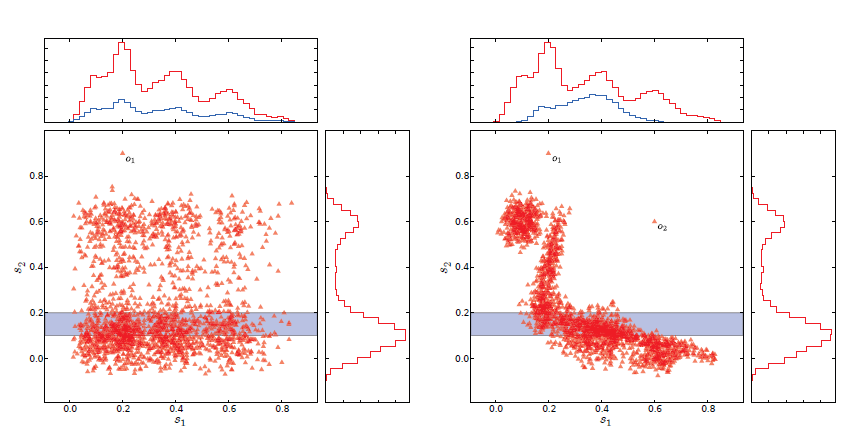
\includegraphics[scale=0.6]{imagenes/ejemplo_anomalia_probabilidad}
	\caption{Ejemplo de anomalía \cite{fabian_keller_hics:_2012}}
\end{figure}

Como se puede observar tenemos dos espacios: el izquierdo no presenta datos correlados y el derecho sí presenta correlación. Podemos ver que en ambos casos se comparte una anomalía etiquetada como $O_1$. Esta anomalía en el caso del espacio no correlado es perfectamente detectable de forma trivial observando las proyecciones de los datos en una dimensión. En cambio en el segundo caso ninguna de las dos anomalías etiquetadas $O_1 , O_2$ son detectables de esta forma trivial, pues si hacemos las proyecciones uno dimensionales ninguno de los dos datos es discordante en dichas proyecciones. Estas anomalías son las que decimos que son no triviales. En cambio si observamos los datos en una proyección de orden superior como la que estamos viendo de dimensión 2 podemos observar claramente que se salen de la correlación de datos que muestra el resto. Es aquí donde podemos ver que en el conjunto de la derecha ninguno de los puntos es una anomalía en las proyecciones de dimensión uno pero sí lo son en la proyección de dimensión 2.

Vamos por tanto a definir más formalmente este concepto especial de anomalía. Necesitamos introducir en primer lugar un poco de notación.

Partimos de un conjunto de datos $X = \{ x_1 , ... , x_n \}$ de $n$ objetos cada uno tomando $d$ valores, es decir, $x_i = (x_{s_1} , ... , x_{s_d}) \in \mathbb{R}^d$. Notamos un subespacio del conjunto de valores como:

$$S = \{ s_i | s_i \in \{ s_1 , ... , s_d \} \ con \ i\in \Delta \}$$

Dado un subespacio $S = \{ s_1 , ... , s_p \}$ notamos la proyección de los objetos del conjunto de datos como $X_{S} = \{ x_{s_1} , ... , x_{s_p} \}$.

Esta proyección está distribuida según una distribución conjunta desconocida de $S$:

$$p_{s_1 , ... , s_p} (x_{s_1} , ... , x_{s_p})$$

Notamos la distribución marginal asociada al atributo $s_i$ como:

$$p_{s_i}(x_{s_i})$$

\begin{definicion}
	Decimos que un subespacio $S$ es un espacio incorrelado si y sólo si:
	
	$$p_{s_1 , ... , s_p}(x_{s_1} , ... , x_{s_p}) = \prod_{i=1}^{p}p_{s_i}(x_{s_i})$$
\end{definicion}

Por tanto si estamos bajo la suposición de un espacio incorrelado podemos decir que la densidad esperada es:

$$p_{esp}(x_{s_1} , ... , x_{s_p}) \equiv \prod_{i=1}^{p}p_{s_i}(x_{s_i})$$

Recordemos que nuestras anomalías no triviales no están en este tipo de subespacios, si no en los correlados. Por tanto vamos a definirlo de la siguiente forma:

\begin{definicion}
	Decimos que un objeto $x_{S}$ es una anomalía no trivial respecto al subespacio $S$ si:
	
	$$p_{s_1 , ... , s_p}(x_{s_1} , ... , x_{s_p}) \ll p_{esp}(x_{s_1} , ... , x_{s_p})$$
	
	Es decir, si la probabilidad esperada es significativamente mayor que la probabilidad conjunta.
\end{definicion}

Por cómo hemos definido los espacios correlados e incorrelados es claro que no podemos tener anomalías en espacios no correlados como es evidente pues la densidad conjunta y esperada serían iguales.

Este concepto como podemos observar no comparte ninguna relación con nuestra definición de anomalías basadas en distancias por lo que es de esperar que si comparamos ambos tipos de anomalías en un conjunto de datos no obtengamos los mismos objetos.
%
\chapter{Redes Neuronales y Deep Learning}
\label{chapter:redes-neuronales-deep-learning}

En este capítulo vamos a dar un repaso a la teoría básica de Redes Neuronales y Deep Learning antes de entrar en la práctica. Repasaremos los fundamentos del aprendizaje con Redes Neuronales, veremos las estructuras de Aprendizaje Profundo o Deep Learning así como las capas de dichas redes que emplearemos en la práctica. Por último veremos una estructura de red que será utilizada en algunos de los modelos, los Autoencoders.

Para la elaboración de este capítulo nos basaremos en los libros de Bengio \cite{goodfellow_deep_2016} y Zaccone \cite{giancarlo_deep_2017}.

\section{Aprendizaje de las Redes Neuronales}

No todas las redes que vamos a emplear en la parte práctica corresponden al modelo ``Feedforward'', ya que también vamos a elaborar redes neuronales con capas recurrentes, pero vamos a estudiar el comportamiento primero de estas redes para luego explicar las modificaciones que dichas arquitecturas añaden.

En primer lugar, llamamos a este tipo de redes prealimentadas o ``Feedforward'' en inglés, porque la información fluye siempre en un sentido, desde la entrada hasta la salida obtenida. En las redes denominadas como recurrentes este sentido de la información se revierte en algunos puntos, realimentando la red con la propia salida de algunas capas o de todas ellas.

La representación más común de una red neuronal profunda es a través de la composición de funciones. Supongamos que estamos aproximando la función $f*(x)$ con una función $f(x)$ construida mediante tres funciones distintas: $f^{(1)}, f^{(2)} \ y \ f^{(3)}$ en este mismo orden. Entonces la representación de la función $f$ quedaría como:

$$f(x) = f^{(3)}(f^{(2)}(f^{(1)}(x))),$$

donde $x$ es la entrada de la red neuronal o lo que es lo mismo, una instancia o varias de nuestro conjunto de datos. En este caso además decimos que $f^{(1)}$ es la primera capa de la red, $f^{(2)}$ la segunda capa, etcétera.

Este tipo de estructuras se llaman profundas al tener varias capas y por tanto varias funciones que, al componerlas, aproximarán la función objetivo que tenemos. Las capas que se encuentran entre la primera y la última, al no ser capas ``visibles'' desde el exterior de la red las denominamos capas ocultas.

Estas capas están compuestas de unidades que denominamos neuronas haciendo una equivalencia con el modelo biológico. Una neurona recibe un número de entradas fijado, por ejemplo $n$. Para cada una de las entradas que recibe va aprendiendo un peso $w$, que luego multiplicará a cada una de las entradas y sumará para obtener un valor ponderado. A este valor ponderado se le aplica una función de activación que nos convierte dicho valor al rango que nosotros queramos para nuestro problema. Por tanto, una neurona produce como salida la función de activación aplicada a una combinación lineal de las entradas que recibe.

\begin{figure}[H]
	\centering
	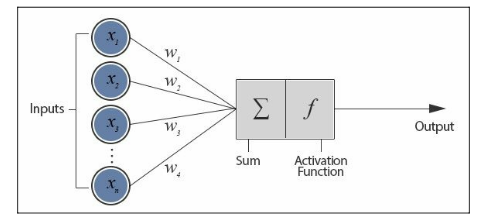
\includegraphics[scale=0.65]{imagenes/neurona.png}
	\caption{Representación de una neurona en una Red Neuronal.}
	\label{img:neurona}
\end{figure}

Como un detalle más a tener en cuenta, solemos añadir a las entradas una que denominamos como sesgo. Este sesgo es 1 y se suma a la combinación lineal, haciendo de término independiente en la ecuación de la recta que se está representando en el espacio de dominio de las instancias.

En cuanto a funciones de activación tenemos muchas sobre las que escoger, veamos las más comunes:

\begin{itemize}
	\item Rectified Linear Unit (ReLU): esta función de activación se define como 
	$$ReLU(x) = x^+ = max(0,x) \ , \ x\in \mathbb{R}^d,$$
	es decir, cero en los negativos y la función identidad en los positivos.
	\begin{figure}[H]
		\centering
		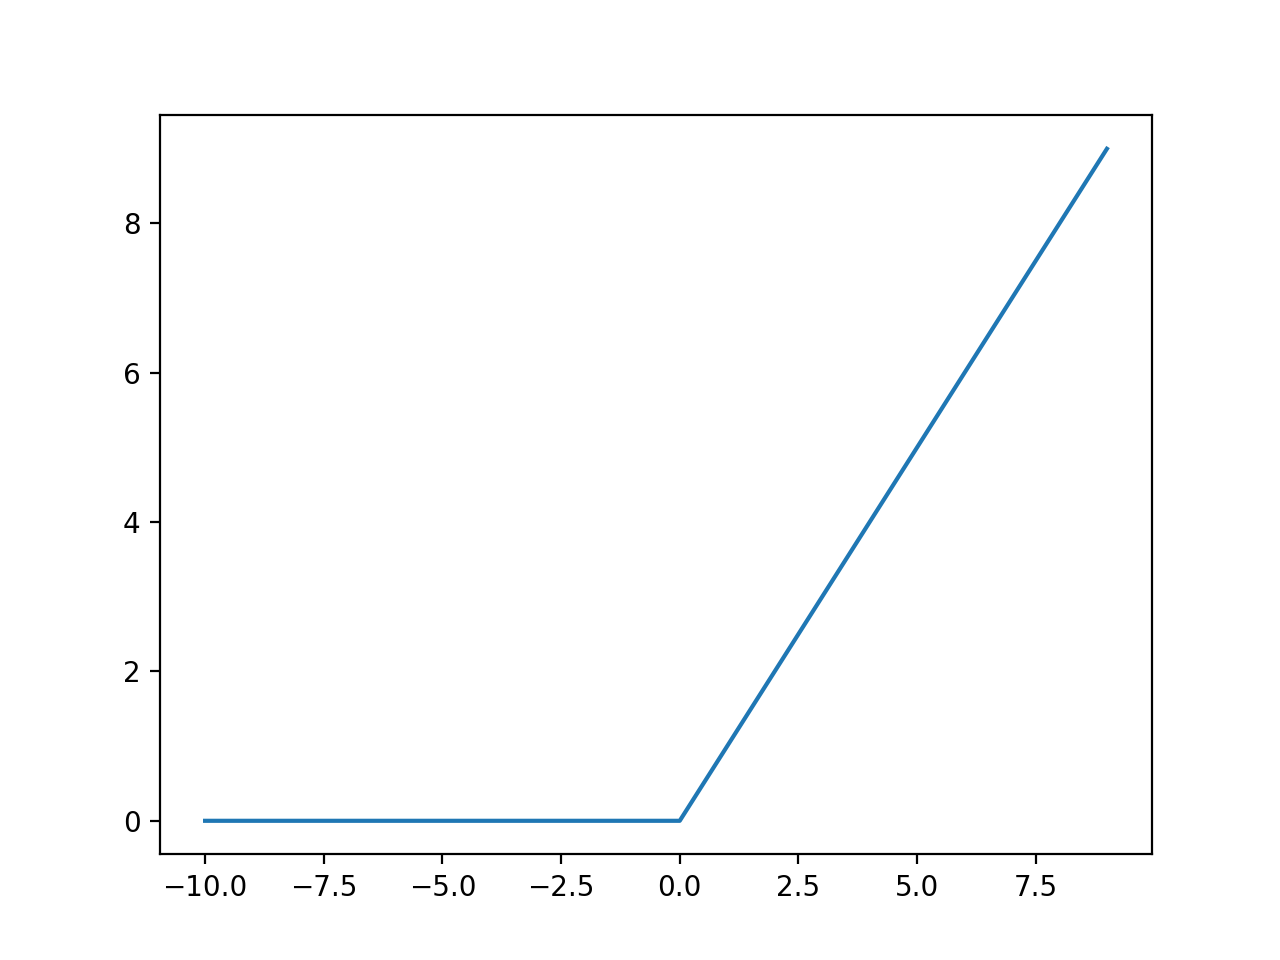
\includegraphics[scale=0.5]{imagenes/relu.png}
		\caption{Función ReLU.}
		\label{img:relu}
	\end{figure}
	\item Softmax: esta función de activación se define como:
	$$softmax : \mathbb{R}^d \rightarrow [0,1]^d$$
	$$softmax(x)_j = \frac{e^{x_j}}{\sum_{k=1}^{d}e^{x_k}}$$
	Con esta función se obtiene un valor con el mismo número de dimensiones que el que tuvieran los datos de entrada. Además, la salida se puede emplear para representar una distribución de probabilidad. Normalmente esta función de salida se emplea en problemas de clasificación donde vamos a obtener un valor entre 0 y 1 para cada una de las clases, siendo el mayor de estos la clase que el modelo predice.
	\item Sigmoide: esta función de activación se define como:
	$$sigmoide(x) = \frac{1}{1+e^{-x}}$$
	Esta función es una función real de variable real muy conocida y estudiada en matemáticas, con propiedades interesantes como que posee dos asíntotas horizontales y tiene una primera derivada no negativa.
	\begin{figure}[H]
		\centering
		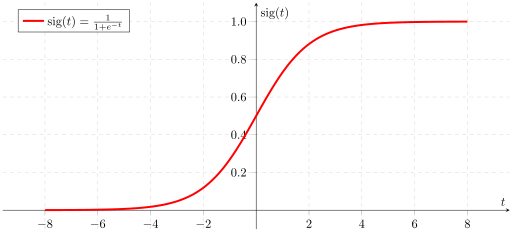
\includegraphics[scale=0.5]{imagenes/sigmoide.png}
		\caption{Función Sigmoide.}
		\label{img:sigmoide}
	\end{figure}
	Su valor máximo es $1$ y su valor mínimo es $0$.
	\item Tangente hiperbólica: la función tangente hiperbólica se define como:
	$$tanh : \mathbb{R}\rightarrow \mathbb{R} \ , \ tanh(x) = \frac{sinh(x)}{cosh(x)} = \frac{e^x - e^{-x}}{e^x + e^{-x}}$$
	\begin{figure}[H]
		\centering
		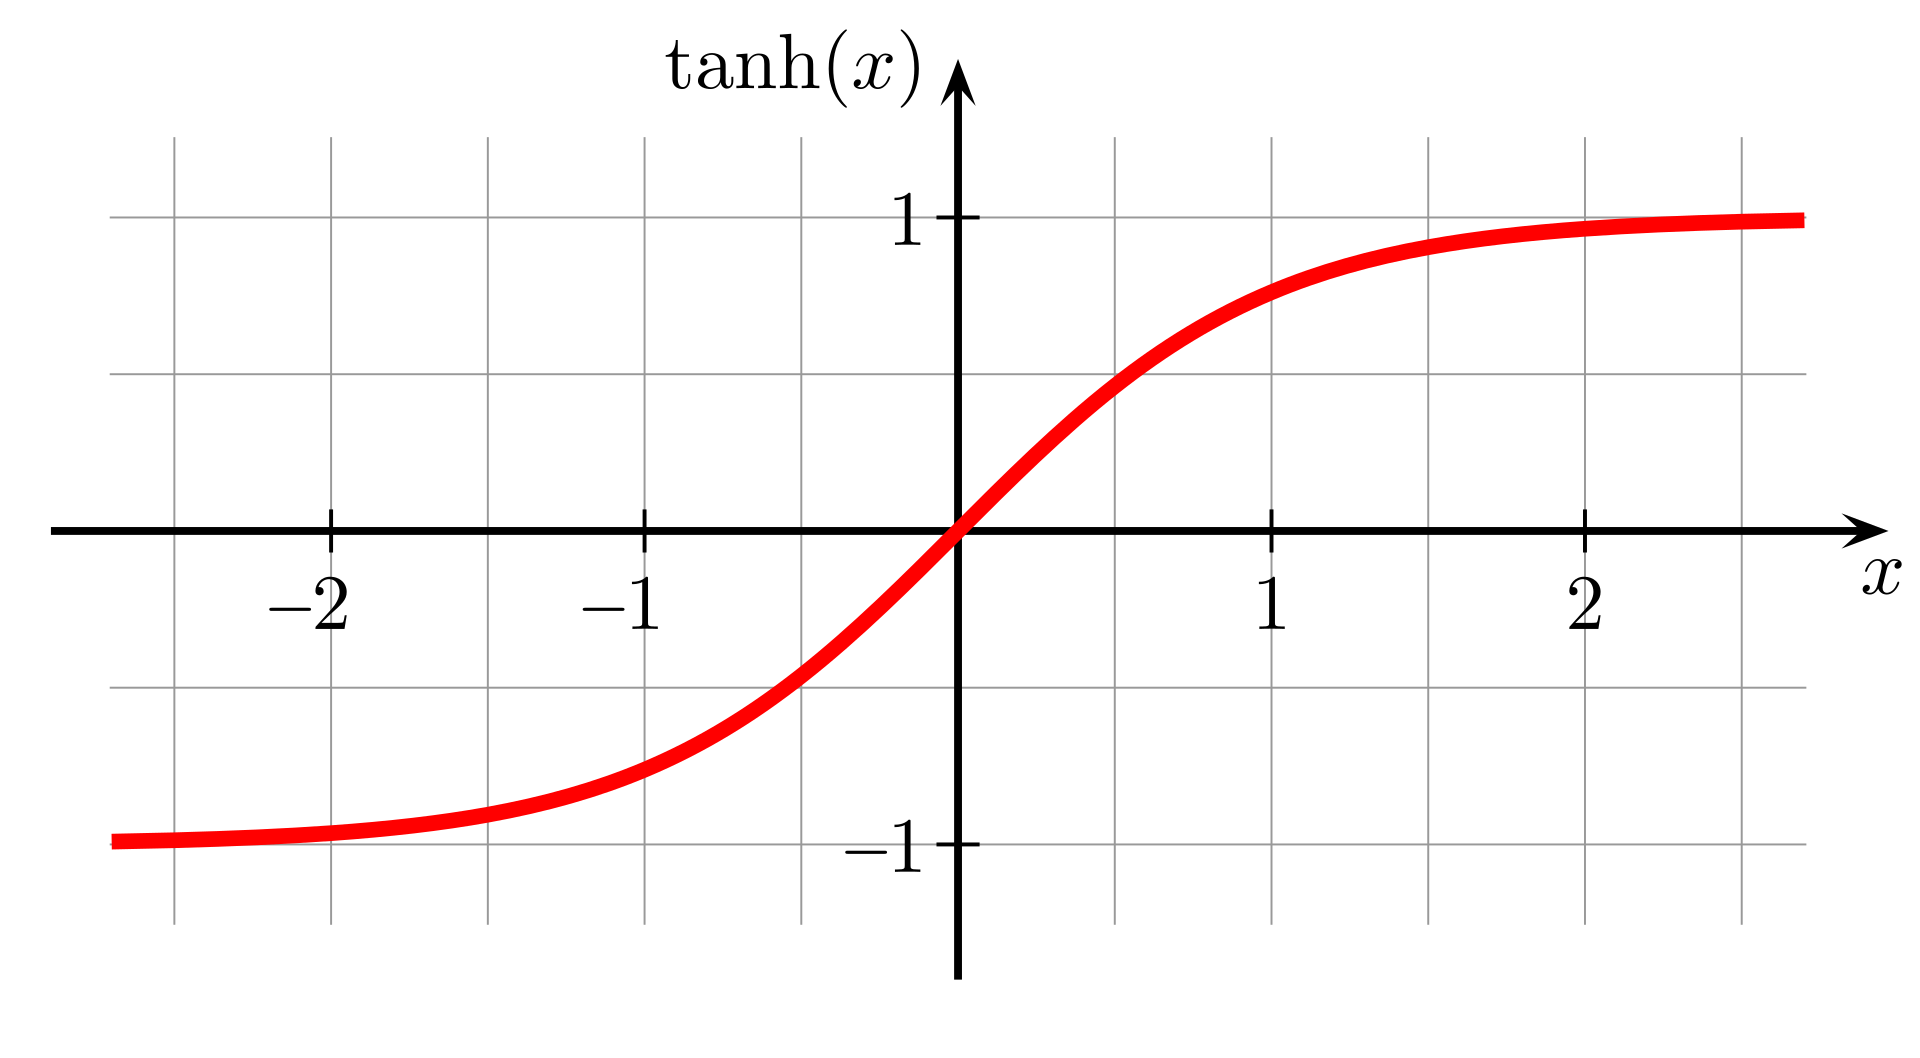
\includegraphics[scale=0.15]{imagenes/tangente_hiperbolica.png}
		\caption{Función tangente hiperbólica.}
		\label{img:tanh}
	\end{figure}
	Como podemos ver esta función de activación puede tomar valores en el intervalo $(-1,1)$.
\end{itemize}

Una vez que sabemos cuál es el comportamiento básico de una neurona vamos a ver cómo funciona el algoritmo empleado en el aprendizaje de las redes: Backpropagation.

Si describimos el proceso de forma sencilla podemos resumirlo en 4 pasos:

\begin{enumerate}
	\item Inicializar la red con pesos aleatorios.
	\item Calcular el error cometido en la predicción con los pesos actuales (pasada hacia delante) y, para cada una de las capas, ir volviendo hacia atrás desde la salida hasta la entrada.
	\item Enseñarle a la red el valor que debía predecir.
	\item Modificar los pesos en cada capa para mejorar la predicción.
\end{enumerate}

Lo primero que tenemos que hacer es definir las funciones de coste. Cuando estamos entrenando una red neuronal queremos tener una función de coste que optimizar, como hemos visto antes en la sección de Machine Learning. En este sentido podemos emplear varias funciones de coste en función de nuestras necesidades, pero es importante tener en cuenta que vamos a necesitar una para el proceso de aprendizaje.

En los cuatro pasos que hemos descrito, tras la inicialización de los pesos, tenemos el paso de la propagación hacia delante. Veamos este paso en pseudocódigo:

\begin{algorithm}[H]{\Large{\textbf{Propagación hacia delante}}}
	
	\vspace{15px}
	
	\caption{Propagación hacia delante}
	\label{alg:forward-propagation}
	\KwIn{Profundidad de la red $l$}
	\KwIn{Matriz de pesos para la capa i-ésima $W^{(i)}$}
	\KwIn{Vector de sesgos de la capa i-ésima $b^{(i)}$}
	\KwIn{Instancia a procesar $x$}
	\KwIn{Salida objetivo $y^*$}
	\KwIn{Función de activación $g$}
	\KwIn{Función de similitud $L$}
	\KwIn{Función de regularización $\Omega$}
	\KwIn{Parámetros del modelo $\theta$}
	\KwIn{Ponderación de la regularización $\lambda$}
	
	\vspace{10px}
	
	$h^{(0)}\leftarrow x$
	
	\For{$k=1,...,l$}{
		
		$z^{(k)}\leftarrow W^{(k)}h^{(k-1)} + b^{(k)}$
		
		$h^{(k)}\leftarrow g(z^{(k)})$
		
	}

	$y\leftarrow h^{(l)}$
	
	$J\leftarrow L(y,y^*) + \lambda \Omega (\theta)$
	
	\vspace{10px}
	
	\KwOut{Predicción hecha $y$}
	\KwOut{Error cometido $J$}
	
	\vspace{5px}
\end{algorithm}

Como podemos ver, este algoritmo se encarga de ir pasando la información desde la entrada (la propia instancia) por cada una de las capas, multiplicando por su peso correspondiente, sumando el sesgo y aplicando la función de activación hasta que obtenemos una salida final.

Hemos visto en las secciones de Machine Learning que, una forma de hacer que nuestros algoritmos aprendan, es necesario obtener el gradiente del error para poder avanzar en el aprendizaje. Para realizar esta labor tenemos el algoritmo Backpropagation, que nos ayudará a calcular dicho gradiente de forma eficiente. Pensemos que tenemos que calcular el gradiente del modelo derivando con respecto a todos los parámetros. Cuando hablamos de Deep Learning es común tener muchas capas ocultas con un número elevado de neuronas, lo que aumenta muchísimo el número de parámetros y por tanto la complejidad del cálculo del gradiente.

Vamos a poner un ejemplo para poder ver la complejidad del cálculo del gradiente:

\begin{figure}[H]
	\centering
	\begin{tikzpicture}[scale=0.2]
		\tikzstyle{every node}+=[inner sep=0pt]
		\draw [black] (34,-24.7) circle (3);
		\draw [black] (34,-38.8) circle (3);
		\draw [black] (48.7,-33) circle (3);
		\draw (15.2,-24.7) node {$x_1$};
		\draw (15.2,-38.8) node {$x_2$};
		\draw (61.1,-33) node {$f$};
		\draw (23.8,-13.6) node {$1$};
		\draw (41.5,-13.6) node {$1$};
		\draw [black] (36.79,-37.7) -- (45.91,-34.1);
		\fill [black] (45.91,-34.1) -- (44.98,-33.93) -- (45.35,-34.86);
		\draw (43.4,-36.44) node [below] {$w_{12}^{(2)}$};
		\draw [black] (36.61,-26.18) -- (46.09,-31.52);
		\fill [black] (46.09,-31.52) -- (45.64,-30.7) -- (45.15,-31.57);
		\draw (39.21,-29.35) node [below] {$w_{11}^{(2)}$};
		\draw [black] (17.6,-26.5) -- (31.6,-37);
		\fill [black] (31.6,-37) -- (31.26,-36.12) -- (30.66,-36.92);
		\draw (19.45,-29.25) node [below] {$w_{21}^{(1)}$};
		\draw [black] (17.6,-37) -- (31.6,-26.5);
		\fill [black] (31.6,-26.5) -- (30.66,-26.58) -- (31.26,-27.38);
		\draw (22.75,-33.50) node [below] {$w_{12}^{(1)}$};
		\draw [black] (51.7,-33) -- (58.1,-33);
		\fill [black] (58.1,-33) -- (57.3,-32.5) -- (57.3,-33.5);
		\draw [black] (25.83,-15.81) -- (31.97,-22.49);
		\fill [black] (31.97,-22.49) -- (31.8,-21.56) -- (31.06,-22.24);
		\draw (31.36,-16.61) node [left] {$b_1^{(1)}$};
		\draw [black] (42.54,-16.41) -- (47.66,-30.19);
		\fill [black] (47.66,-30.19) -- (47.85,-29.26) -- (46.91,-29.61);
		\draw (44.34,-24.11) node [left] {$b_1^{(2)}$};
		\draw [black] (24.93,-16.38) -- (32.87,-36.02);
		\fill [black] (32.87,-36.02) -- (33.04,-35.09) -- (32.11,-35.47);
		\draw (25.16,-20.1) node [left] {$b_2^{(1)}$};
		\draw [black] (18.2,-24.7) -- (31,-24.7);
		\fill [black] (31,-24.7) -- (30.2,-24.2) -- (30.2,-25.2);
		\draw (24.6,-25.2) node [below] {$w_{11}^{(1)}$};
		\draw [black] (18.2,-38.8) -- (31,-38.8);
		\fill [black] (31,-38.8) -- (30.2,-38.3) -- (30.2,-39.3);
		\draw (24.6,-39.3) node [below] {$w_{22}^{(1)}$};
	\end{tikzpicture}
	\label{fig:backpropagation-ejemplo}
	\caption{Ejemplo de una red neuronal sencilla.}
\end{figure}

Aquí podemos ver una red neuronal con 2 entradas y dos capas. Cada una de las capas tiene sus pesos y sus sesgos correspondientes. Entonces, en el modelo que hemos puesto como ejemplo, tenemos el siguiente vector de parámetros que determina nuestra red neuronal:

$$\theta = \Big(w_{11}^{(1)}, w_{12}^{(1)}, w_{21}^{(1)}, w_{22}^{(1)}, b_1^{(1)}, b_2^{(1)}, w_{11}^{(2)}, w_{12}^{(2)}, b_1^{(2)}\Big)$$

Con estos parámetros, la expresión de la salida de la red neuronal es:

$$f(x_1 , x_2 ; \theta) = g(w_{11}^{(2)}g(w_{11}^{(1)}x_1 + w_{12}^{(1)}x_2 + b_1^{(1)}) + w_{12}^{(2)}g(w_{21}^{(1)}x_1 + w_{22}^{(1)}x_2 + b_2^{(1)}) + b_1^{(2)})$$

Para simplificar las expresiones de las parciales vamos a notar lo siguiente:

$$\alpha = g' (w_{11}^{(2)}g(w_{11}^{(1)}x_1 + w_{12}^{(1)}x_2 + b_1^{(1)}) + w_{12}^{(2)} g(w_{21}^{(1)}x_1 + w_{22}^{(1)}x_2 + b_2^{(1)}) + b_1^{(2)}),$$

$$\beta =  g'(w_{11}^{(1)}x_1 + w_{12}^{(1)}x_2 + b_1^{(1)}) \ y$$

$$\gamma =  g'(w_{21}^{(1)}x_1 + w_{22}^{(1)}x_2 + b_2^{(1)}).$$

Con esto, podemos sacar las parciales de f, que nos van a ser necesarias en el cálculo del gradiente del coste J.

\footnotesize
\begin{alignat*}{3}
\frac{\partial f}{\partial w_{11}^{(1)}}(x_1,x_2;\theta)&=\alpha w_{11}^{(2)}\beta x_1,\quad&
\frac{\partial f}{\partial w_{12}^{(1)}}(x_1,x_2;\theta)&=\alpha w_{11}^{(2)}\beta x_2,\\
\frac{\partial f}{\partial w_{21}^{(1)}}(x_1,x_2;\theta)&=\alpha w_{12}^{(2)}\gamma x_1,\quad&
\frac{\partial f}{\partial w_{22}^{(1)}}(x_1,x_2;\theta)&=\alpha w_{12}^{(2)}\gamma x_2,\\
\frac{\partial f}{\partial b_{1}^{(1)}}(x_1,x_2;\theta)&=\alpha w_{11}^{(2)}\beta, \quad&
\frac{\partial f}{\partial b_{2}^{(1)}}(x_1,x_2;\theta)&=\alpha w_{12}^{(2)}\gamma, \\
\frac{\partial f}{\partial w_{11}^{(2)}}(x_1,x_2;\theta)&=\alpha g(w_{11}^{(1)}x_{1}+w_{12}^{(1)}x_2 + b_1^{(1)}),&&\\
\frac{\partial f}{\partial w_{12}^{(2)}}(x_1,x_2;\theta)&=\alpha g(w_{21}^{(1)}x_{1}+w_{22}^{(1)}x_2 + b_2^{(1)}),&\quad
\frac{\partial f}{\partial b_{1}^{(2)}}(x_1,x_2;\theta)&=\alpha.
\end{alignat*}
\normalsize

Viendo las expresiones que tenemos de las derivadas parciales se puede entender mejor la necesidad de eficiencia. En primer lugar, podemos ver que no tenemos una red para nada grande y ya tenemos que calcular 9 derivadas parciales. Por otro lado, podemos ver que hay términos que se repiten bastante con lo que, calculando primero estos términos, simplificamos la complejidad computacional de este problema.

Veamos el algoritmo de Backpropagation en pseudocódigo:

\begin{algorithm}[H]{\Large{\textbf{Propagación hacia atrás}}}
	
	\vspace{15px}
	
	\caption{Propagación hacia atrás}
	\label{alg:backpropagation}
	
	\vspace{10px}
	
	Calculamos el gradiente de la capa de salida.
	
	$d\leftarrow \nabla_y J(y,y^*;\theta) = \nabla_y L(y,y^*)$
	
	\For{$k=l,...,1$}{
	
		Aplicamos la regla de la cadena ($\odot$ es el producto componente a componente).
		
		$d\leftarrow \nabla_{z^{(k)}} J = d\odot g' (z^{(k)})$
		
		Calculamos los gradientes en los pesos y sesgos añadiendo también la regularización si la hubiera.
		
		$\nabla_{b^{(k)}}J = d + \lambda \nabla_{b^{(k)}} \Omega (\theta)$
		
		$\nabla_{W^{(k)}}J = d(h^{(k-1)})^T + \lambda \nabla_{W^{(k)}} \Omega (\theta)$
		
		$d\leftarrow \nabla_{h^(k-1)} J = \Big( W^{(k)} \Big)^T d$

	}
	
	\KwOut{Valor final del gradiente $d$}
	
	\vspace{5px}
\end{algorithm}

Como podemos ver, este algoritmo simplemente aplica la regla de la cadena y va calculando los gradientes sin repetir las derivadas capa a capa. Esta aproximación hace que el cálculo sea más sencillo y no se repita.

Llegados a este punto ya tenemos la salida que nos produce nuestra red neuronal con el algoritmo de propagación hacia delante y tenemos el cálculo del gradiente con la propagación hacia atrás. Ahora nos queda optimizar dicho coste con las herramientas que tenemos, es decir, resolver el problema de optimización que tenemos con el gradiente. 

Para resolver este problema tenemos la aproximación clásica de Gradiente Descendente Estocástico aunque no es la única herramienta que podemos usar para esto. Veremos algunas de las más utilizadas y cómo nos ayudan para obtener nuevos parámetros que mejoren el desempeño de las redes.

En primer lugar cabe explicar el algoritmo más empleado en esta tarea: Gradiente Descendente Estocástico. En Deep Learning se emplea el entrenamiento por lotes o batches en inglés, lo que hace inviable el uso de ténicas como Gradiente Descendente. Es por ello que se suele emplear la aproximación estocástica de Gradiente Descendente al ir calculando una aproximación del gradiente con números pequeños de muestras. Veamos el algoritmo en pseudocódigo:

\begin{algorithm}[H]{\Large{\textbf{Gradiente Descendente Estocástico en la iteración k-ésima}}}
	
	\vspace{15px}
	
	\caption{Gradiente Descendente Estocástico}
	\label{alg:sgd}
	\KwIn{Tasa de Aprendizaje $\epsilon_k$}
	\KwIn{Parámetros iniciales $\theta$}
	\KwIn{Tamaño de los lotes de datos $m$}
	
	\vspace{10px}
	
	\While{no se cumpla el criterio de parada}{
	
		Escoger un batch de datos de tamaño $m$ $x^{(1)}, ..., x^{(m)}$ con correspondientes objetivos $y^{(1)}, ..., y^{(m)}$
		
		Calculamos una estimación del gradiente.
		
		$\hat{g} \leftarrow \frac{1}{m}\nabla \sum_{i} L(f(x^{(i)};\theta), y^{(i)})$
		
		Actualizamos los parámetros.
		
		$\theta \leftarrow \theta - \epsilon_k \hat{g}$
	
	}
	
	\vspace{10px}
	
	\KwOut{Nuevos parámetros $\theta$}
	
	\vspace{5px}
\end{algorithm}

Como podemos ver, lo que estamos haciendo a cada paso es mejorar los parámetros del modelo en función del gradiente del coste, o más bien en este caso una aproximación del gradiente del coste. 

Con esto ya si tenemos el algoritmo completo: propagación hacia delante para obtener la salida predicha y el error, propagación hacia atrás para obtener el gradiente del coste y Gradiente Descendente Estocástico (u otro método) para optimizar los parámetros del modelo (o lo que es lo mismo, los pesos) hacia el mejor resultado.

También es común emplear variaciones de este algoritmo, pues puede mejorar con respecto a SGD aunque depende siempre del problema y los datos asociados. Las variaciones más comunes de este algoritmo son:

\begin{itemize}
	\item SGD con momento: a veces el algoritmo de Gradiente Descendente y el algoritmo de Gradiente Descendente Estocástico presentan una oscilación alrededor del mínimo de la función que pretenden minimizar. Veamos un ejemplo de esto:
	
	\begin{figure}[H]
		\centering
		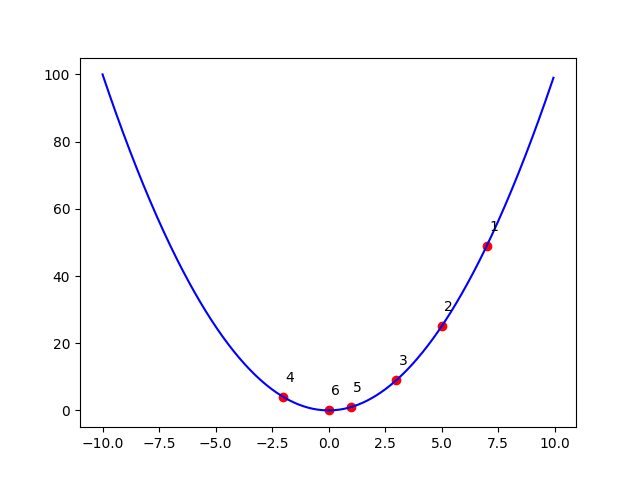
\includegraphics[scale=0.7]{imagenes/sgd.png}
		\caption{Oscilación alrededor del mínimo.}
		\label{img:oscilacion-sgd}
	\end{figure}

	En esta figura podemos ver cómo se produce una oscilación alrededor del mínimo. En funciones más complejas esta oscilación puede ser aún mayor y condicionar el funcionamiento del algoritmo de optimización. Esta variante del algoritmo hace que este zigzagueo u oscilación sea más leve, veamos el algoritmo en pseudocódigo:
	
	\begin{algorithm}[H]{\Large{\textbf{Gradiente Descendente Estocástico con momento}}}
		
		\vspace{15px}
		
		\caption{Gradiente Descendente Estocástico con momento}
		\label{alg:sgd-momento}
		\KwIn{Tasa de Aprendizaje $\epsilon$}
		\KwIn{Parámetros iniciales $\theta$}
		\KwIn{Tamaño de los lotes de datos $m$}
		\KwIn{Momento $\alpha$}
		\KwIn{Velocidad inicial $v$}
		
		\vspace{10px}
		
		\While{no se cumpla el criterio de parada}{
			
			Escoger un batch de datos de tamaño $m$ $x^{(1)}, ..., x^{(m)}$ con correspondientes objetivos $y^{(1)}, ..., y^{(m)}$
			
			Calculamos una estimación del gradiente.
			
			$\hat{g} \leftarrow \frac{1}{m}\nabla \sum_{i} L(f(x^{(i)};\theta), y^{(i)})$
			
			Actualizamos la velocidad.
			
			$v\leftarrow \alpha v - \epsilon \hat{g}$
			
			Actualizamos los parámetros.
			
			$\theta \leftarrow \theta + v$
			
		}
		
		\vspace{10px}
		
		\KwOut{Nuevos parámetros $\theta$}
		
		\vspace{5px}
	\end{algorithm}

	\item AdaGrad: esta es una versión adaptativa de SGD. El algoritmo varía los parámetros de forma inversamente proporcional a la raíz cuadrada de la suma de los cuadrados de los valores anteriores. Es decir, actualiza la tasa de aprendizaje decrementándola más rápido cuanto mayores sean las derivadas parciales. Como consecuencia de esto el avance en el espacio es más rápido que SGD. Veamos el pseudocódigo:
	
	\begin{algorithm}[H]{\Large{\textbf{Adagrad}}}
		
		\vspace{15px}
		
		\caption{Adagrad}
		\label{alg:adagrad}
		\textbf{Notación:} $\odot$ nota el producto componente a componente, $\sqrt{\cdot}$ es la raíz cuadrada componente a componente y las divisiones correspondientes son componente a componente.
		
		\KwIn{Tasa de Aprendizaje $\epsilon$}
		\KwIn{Parámetros iniciales $\theta$}
		\KwIn{Tamaño de los lotes de datos $m$}
		\KwIn{Constante inicial $\delta$ pequeña}
		
		\vspace{10px}
		
		$r\leftarrow 0$
		
		\While{no se cumlpa el criterio de parada}{
		
			Escoger un batch de datos de tamaño $m$ $x^{(1)}, ..., x^{(m)}$ con correspondientes objetivos $y^{(1)}, ..., y^{(m)}$
			
			Calculamos una estimación del gradiente.
			
			$\hat{g} \leftarrow \frac{1}{m}\nabla \sum_{i} L(f(x^{(i)};\theta), y^{(i)})$
			
			$r\leftarrow r + \hat{g}\odot \hat{g}$
			
			$\Delta \theta \leftarrow - \frac{\epsilon}{\delta + \sqrt{r}} \odot \hat{g}$
			
			$\theta \leftarrow \theta + \Delta \theta$

		}
		
		\vspace{10px}
		
		\KwOut{Nuevos parámetros $\theta$}
		
		\vspace{5px}
	\end{algorithm}

	\item RMSProp: en vez de ir acumulando los gradientes se hace una media exponencial, lo que teóricamente mejor el comportamiento al minimizar funciones no convexas (aquellas idóneas para SGD).
	
	\begin{algorithm}[H]{\Large{\textbf{RMSProp}}}
		
		\vspace{15px}
		
		\caption{RMSProp}
		\label{alg:rmsprop}
		\textbf{Notación:} $\odot$ nota el producto componente a componente, $\sqrt{\cdot}$ es la raíz cuadrada componente a componente y las divisiones correspondientes son componente a componente.
		
		\KwIn{Tasa de Aprendizaje $\epsilon$}
		\KwIn{Parámetros iniciales $\theta$}
		\KwIn{Tamaño de los lotes de datos $m$}
		\KwIn{Constante inicial $\delta$ pequeña}
		\KwIn{Tasa de decaimiento $\rho$}
		
		\vspace{10px}
		
		$r\leftarrow 0$
		
		\While{no se cumlpa el criterio de parada}{
			
			Escoger un batch de datos de tamaño $m$ $x^{(1)}, ..., x^{(m)}$ con correspondientes objetivos $y^{(1)}, ..., y^{(m)}$
			
			Calculamos una estimación del gradiente.
			
			$\hat{g} \leftarrow \frac{1}{m}\nabla \sum_{i} L(f(x^{(i)};\theta), y^{(i)})$
			
			$r\leftarrow \rho r + (1-\rho)\hat{g}\odot \hat{g}$
			
			$\Delta \theta \leftarrow - \frac{\epsilon}{\delta + \sqrt{r}} \odot \hat{g}$
			
			$\theta \leftarrow \theta + \Delta \theta$
			
		}
		
		\vspace{10px}
		
		\KwOut{Nuevos parámetros $\theta$}
		
		\vspace{5px}
	\end{algorithm}

	\item Adam: es una modificación de RMSProp con momento. Veamos el pseudocódigo:
	
	\begin{algorithm}[H]{\Large{\textbf{RMSProp}}}
		
		\vspace{15px}
		
		\caption{RMSProp}
		\label{alg:rmsprop}
		\textbf{Notación:} $\odot$ nota el producto componente a componente, $\sqrt{\cdot}$ es la raíz cuadrada componente a componente y las divisiones correspondientes son componente a componente.
		
		\KwIn{Tasa de Aprendizaje $\epsilon$}
		\KwIn{Parámetros iniciales $\theta$}
		\KwIn{Tamaño de los lotes de datos $m$}
		\KwIn{Constante inicial $\delta$ pequeña}
		\KwIn{Tasas de decaimiento $\rho_1 , \rho_2 \in [0,1)$}
		
		\vspace{10px}
		
		$s\leftarrow 0$
		
		$r\leftarrow 0$
		
		$t\leftarrow 0$
		
		\While{no se cumlpa el criterio de parada}{
			
			Escoger un batch de datos de tamaño $m$ $x^{(1)}, ..., x^{(m)}$ con correspondientes objetivos $y^{(1)}, ..., y^{(m)}$
			
			Calculamos una estimación del gradiente.
			
			$\hat{g} \leftarrow \frac{1}{m}\nabla \sum_{i} L(f(x^{(i)};\theta), y^{(i)})$
			
			$t\leftarrow t+1$
			
			$s\leftarrow \rho_1 \cdot s + (1-\rho_1)\hat{g}$
			
			$r\leftarrow \rho_2 \cdot s + (1-\rho_2)\hat{g}\odot \hat{g}$
			
			$\hat{s}\leftarrow \frac{s}{1-\rho_1^r}$
			
			$\hat{r}\leftarrow \frac{r}{1-\rho_2^r}$
			
			$\Delta \theta \leftarrow - \frac{\epsilon}{\delta + \sqrt{\hat{r}}}\hat{s}$
			
			$\theta \leftarrow \theta + \Delta \theta$
			
		}
		
		\vspace{10px}
		
		\KwOut{Nuevos parámetros $\theta$}
		
		\vspace{5px}
	\end{algorithm}
\end{itemize}

Con esto ya hemos cubierto cómo aprende una red neuronal de forma completa.

\section{Capas empleadas}

\subsection{Capas densas o totalmente conectadas}

En las redes neuronales tenemos distintos tipos de capas o neuronas que podemos utilizar en la construcción de la arquitectura de la red. La estructura explicada con anterioridad asumía el uso de capas densas o totalmente conectadas. Estas capas tienen exactamente el comportamiento descrito en la figura \ref{img:neurona}. Debemos tener en cuenta que vamos a emplear un tipo de capa u otro en función de la información que queramos obtener de nuestros datos.

En primer lugar vamos a hacer un pequeño repaso de las capas densas o totalmente conectadas. Estas capas están ya descritas en la sección anterior, por lo que no nos vamos a detener más en esto. Las capas densas son empleadas cuando tenemos entradas de tipo numérico, ya sea una única entrada numérica o un vector de números. 

Lo más común es que esta capa siempre aparezca en la mayoría de estructuras de redes neuronales, pues aunque sea una red por ejemplo con mayoría de capas convolucionales, normalmente las últimas o las primeras son capas densas que nos permiten igualar la dimensión de los datos a lo que nosotros queramos (en función de si es un problema de predicción, regresión o clasificación u otro tipo).

El funcionamiento de este tipo de capas es muy sencillo. Tenemos una neurona que recibe tantas conexiones como neuronas o entradas hubiera en la capa anterior más un sesgo. Todas estas conexiones tienen un peso asignado como vimos en el ejemplo \ref{fig:backpropagation-ejemplo}. Este comportamiento se replica en toda la capa, es decir, todas las neuronas de la capa reciben como entrada todas estas conexiones con un valor numérico y un peso asignado. Estos pesos y valores se combinan de forma lineal, es decir, multiplicando cada valor numérico por cada uno de los pesos y sumándose. Tras la suma simplemente se añade el término de sesgo y se aplica a todo esto la función de activación, que es intrínseca de la capa. Esto quiere decir que, para que el funcionamiento de la capa sea homogéneo, se aplica la misma función de activación a todas las neuronas que componen dicha capa. Esto lo que nos va a producir como salida es un vector de valores numéricos, que son las salidas de cada una de las neuronas de nuestra capa.

\begin{figure}[H]
	\centering
	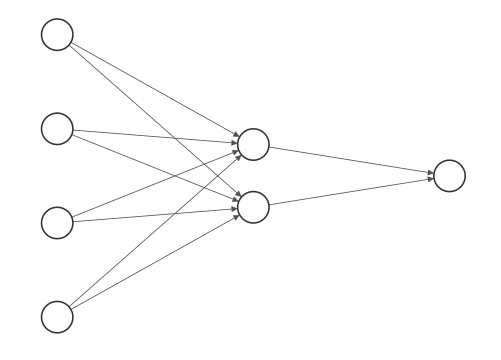
\includegraphics[scale=0.5]{imagenes/fcnn_example.png}
	\caption{Ejemplo de red neuronal con capas densas.}
	\label{img:ejemplo-fcnn}
\end{figure}

En este ejemplo podemos ver que tenemos 3 capas, una capa de entrada, una capa oculta y una de salida. La capa de entrada tiene 4 neuronas, por lo que recibe como entrada un vector numérico de 4 valores que se asocian cada uno con una neurona. La capa oculta tiene 2 neuronas que reciben como entrada cada una un vector numérico de 4 valores, produciendo dicha capa al final un vector de dos valores numéricos. Por último la capa de salida tiene una única neurona, por lo que la salida de la red es un único valor numérico, recibiendo como entrada un vector de dos valores.

Esta capa nos servirá en todas las estructuras Deep Learning elaboradas que emplearemos más tarde en la aplicación práctica.

\subsection{Capas convolucionales}

En esta sección vamos a explicar el funcionamiento de las capas de convolución, los datos que reciben y los datos que obtenemos a través de la operación de convolución.

Lo primero que tenemos que hacer es definir el operador de convolución para poder ver cómo y donde emplearlo en una red neuronal. Supongamos que tenemos una serie de datos que dependen de una variable $t$ temporal, es decir, por ejemplo podemos tener distintos valores de una serie temporal. Si la función que nos da dichos valores de la serie temporal es $x(t)$, podemos definir una función que suavice a $x(t)$ de la siguiente forma:

$$s(t) = \int x(a)\cdot w(t-a) da = (x * w)(t)$$

Donde $w(a)$ es una ponderación que hacemos a los valores de la función $x(t)$. Además, se suele notar esta operación con el asterisco como hemos hecho. Esta función suavizada de la original es lo que llamamos operación de convolución.

En un caso real de aplicación no vamos a tener la función $x(t)$ que nos da la salida u objetivo de nuestro problema en cada instante de tiempo, pues entonces no habría problema al estar resuelto y modelado. Por contra, lo que vamos a tener normalmente es una serie de valores de ejemplo de salida. Al ser este un número finito de muestras, sabemos que la integral se define como una suma y por tanto podemos definir el operador de convolución como:

$$s(t) = (x*w)(t) = \sum_{a=-\infty}^{\infty}x(a)w(t-a)$$

Está claro que esta definición que hemos dado no tiene sentido cuando tenemos más de un valor, es decir, cuando la función $x$ no es real, si no que da como salida un vector de números.

Normalmente empleamos como entrada en este tipo de redes con capas convolucionales un array de datos, por ejemplo, una imagen o varias instancias de una serie temporal. Esto hace que tengamos como input una matriz bidimensional o tridimensional normalmente como entrada, por lo que tenemos que pensar en hacer la operación de convolución en varios ejes. La aplicación de esta operación nos va a dar como resultado de nuevo una matriz, como es natural. Por tanto, suponiendo que $I$ es nuestra imagen de entrada o grupo de datos de una serie temporal, podemos definir el operador de convolución sobre dos ejes como:

$$S(i,j) = (I*K)(i,j) = \sum_{m} \sum_{n} I(m,n)K(i-m,j-n)$$

Donde K es un núcleo o kernel de dos dimensiones, como la entrada, pero no tiene por qué tener el mismo tamaño que la misma. Como característica de esta operación tenemos que es conmutativa, es decir, $(I*K)(i,j) = (K*I)(i,j)$ al invertirse únicamente el producto que tenemos dentro de la sumatoria.

Veamos un ejemplo de como aplicamos esta operación de convolución a una matriz de dos dimensiones $3x4$ con un kernel $2x2$:

\begin{figure}[H]
	\centering
	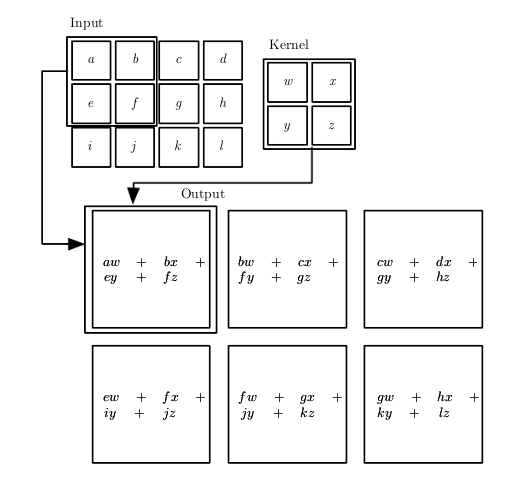
\includegraphics[scale=0.65]{imagenes/convolucion.png}
	\caption{Ejemplo de operación de convolución.}
	\label{img:convolucion}
\end{figure}

Como podemos ver, el resultado de esta operación es tomar el kernel e ir deslizándolo por la matriz para obtener, por cada una de estas posiciones, un valor real y construir de esta forma una matriz de salida. En este caso, con un kernel $2x2$ y con una matriz de entrada $3x4$ obtenemos una matriz de salida $2x3$.

Precisamente en este tipo de capas, los pesos son los núcleos que aplicamos en la operación de convolución, por lo que nuestro algoritmo de backpropagation se orientará en optimizar dichos valores.

Normalmente, una capa de convolución dentro de una red neuronal hace esta operación de convolución con varios filtros o kernels, por ejemplo 32, 64, 128 u otro número. Si elegimos tamaño de kernel $3x3$ entonces tendríamos 32, 64, 128 u otro número de matrices con 9 pesos en cada una que entrenaremos con backpropagation.

Con esta capa de convolución se suele combinar una capa u operador de Pooling o agrupación. Este operador nos va a servir para agrupar los datos y reducir la dimensión. El operador de agrupación se aplica a cada una de las salidas de la convolución, es decir, al resultado de hacer $(I*K)$ con cada uno de los núcleos. Podemos aplicar aquí por ejemplo un agrupamiento $2x2$ que nos reducirá la dimensión de la salida a la mitad para cada núcleo.

Esta operación, a parte de reducir la dimensión de la salida, nos va a ayudar a que nuestra salida sea más robusta. Pensemos por ejemplo en que tenemos imágenes como datos de entrada, si las imágenes de entrada varían ligeramente (una ligera traslación) entonces la operación de Pooling nos va a ayudar a que la información que extraemos sea invariante frente a estas pequeñas variaciones.

Las dos operaciones de agrupamiento que se suelen emplear en la capa de Pooling son el máximo y la media. Esto lo que hace es obtener como valor final la media o el máximo del tamaño de Pooling que estemos haciendo. Pensemos por ejemplo que la salida de la convolución es una matriz $8x8$ y nosotros hacemos un agrupamiento $2x2$. Entonces vamos a ir pasando por la salida una matriz $2x2$ y calculando la media o el máximo de dicha matriz para obtener un único valor, después desplazamos uno a la derecha y hacia abajo una unidad también cuando acabemos la fila completa. De esta forma iremos construyendo una matriz con los máximos o medias de la salida de la convolución.

Ya que entendemos un poco mejor cómo funciona la operación de convolución y cómo funcionan las capas convolucionales y de agrupamiento, vamos a repasar brevemente el objetivo y el uso de estas capas en la redes neuronales. 

Para poder aplicar la operación de convolución de forma coherente debemos tener datos que tengan una dependencia local, por ejemplo las imágenes o una serie temporal sobre la que agrupamos las instancias consecutivas en el tiempo para formar un vector (en el caso de una serie temporal real) o una matriz (en el caso de una serie temporal de varias variables de salida). 

Con la operación de convolución, al ir repitiendo esta operación varias veces junto con el agrupamiento, obtenemos información local interesante e importante para nuestro problema. Por ejemplo sería algo común que, tras la aplicación de varias capas de convolución, obtuviéramos como salida de esos parches formas, objetos o secciones de imágenes que sean de relevancia para nuestra tarea final. Esto ocurre de igual forma con las series temporales u otro tipo de datos, pero es más sencillo explicar este fenómeno con las imágenes por la capacidad de visualizar los datos.

Por tanto estas capas no están pensadas para ser la última o primera capa de nuestra red, si no para formar parte de ella para obtener características de nuestros datos que nos ayuden en la tarea de predicción, regresión o clasificación que tengamos como objetivo.

\subsection{Capas recurrentes y LSTM}

Este tipo de redes y capas están pensadas precisamente para recibir como entrada varias instancias consecutivas en el tiempo de una serie temporal. Para poder hacer una red con un mejor desempeño en este tipo de datos, vamos a hacer que los pesos de una capa en un momento determinado de la serie temporal, puedan afectar a momentos posteriores y capas posteriores dependiendo de la estructura de la red. Con ello, la intención es poder sacar patrones que no dependan del tiempo y sean poco sensibles a variaciones como reflexiones de los datos (cambiar inicio por fin y fin por inicio) y procesar datos de distinto tamaño.

En este tipo de datos siempre tenemos una dependencia de los datos con los anteriores en el tiempo, es decir, podemos describir el dato en el instante $t$ de tiempo a partir de los datos en los instantes anteriores. Supongamos que tenemos representado el estado del sistema como $s^{(t)}$ entonces esto se traduce en que:

$$s^{(t)} = f(s^{(t-1)};\theta),$$

es decir, el valor en el instante $t$ depende del $t-1$ y así sucesivamente. En una aplicación real de este tipo de redes, fijamos un número de pasos en el tiempo que vamos a analizar en bloque. Por tanto este proceso recurrente se puede desarrolla de forma extensiva. Si fuese con 3 pasos en el tiempo tendríamos que $s^{(3)}$ se podría expresar como:

$$s^{(3)} = f(s^{(2)};\theta) = f(f(s^{(1)};\theta);\theta)$$

Ahora vamos a hacer este ejemplo algo más real. Supongamos que tenemos nuestro sistema $h(t)$ (se nota con h porque será oculto dentro de la red, hidden) y una señal externa (la serie temporal) entonces podemos describir nuestro sistema dinámico recurrente como:

$$h^{(t)} = f(h^{(t-1)},x^{(t)};\theta)$$

Esta función que modela nuestro sistema con el estado del mismo y con una señal externa la podemos desenrollar, es decir, eliminar la componente recurrente al estar basado en un número finito de muestras como hemos hecho anteriormente.

\begin{figure}[H]
	\centering
	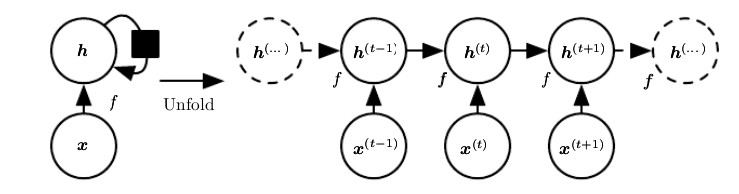
\includegraphics[scale=0.5]{imagenes/desenrollado.png}
	\caption{Desenrollado de la función recurrente.}
	\label{img:desenrollado-recurrente}
\end{figure}

Como podemos ver en el esquema, el estado anterior del sistema influye sobre el estado actual y la señal exterior actual influye también en el estado del sistema.

Con esta idea de compartir pesos y que el estado actual vaya dependiendo de los anteriores, llevando una dependencia temporal, podemos elaborar distintos tipos de redes neuronales.

\begin{figure}[H]
	\centering
	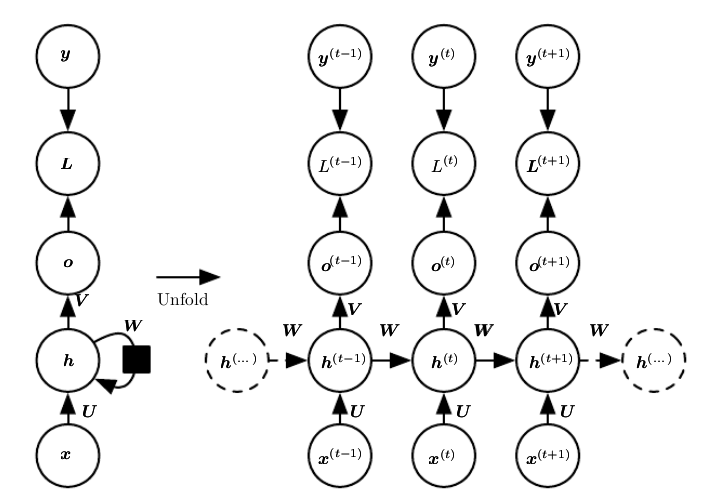
\includegraphics[scale=0.5]{imagenes/rnn1.png}
	\caption{Red recurrente que produce una salida en cada paso temporal con conexiones entre las unidades ocultas.}
	\label{img:red-recurrente1}
\end{figure}

En este caso vemos un esquema, en el que tenemos las entradas o estímulos externos que describíamos anteriormente, el estado interno del sistema representado con $h$, la salida producida $o$, la función de pérdida de la salida predicha frente a la real $L$ y la salida real $y$.

En este tipo de red neuronal tenemos la entrada ponderada por unos pesos $U$, el estado interno ponderado por pesos $W$ y la salida ponderada por pesos $V$. Podemos ver que esta estructura nos da, para cada unidad de tiempo, su salida correspondiente y  como podemos ver, los pesos de la capa oculta solo se usan de un instante de tiempo a otro de la misma capa oculta o estado del sistema.

\begin{figure}[H]
	\centering
	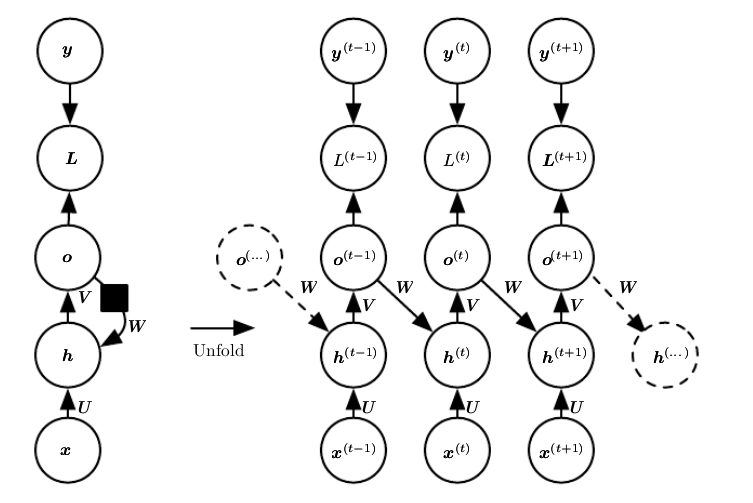
\includegraphics[scale=0.5]{imagenes/rnn2.png}
	\caption{Red recurrente que produce una salida en cada paso temporal con conexiones de la salida a las unidades ocultas.}
	\label{img:red-recurrente2}
\end{figure}

En este caso podemos ver como no hay conexiones de pesos entre las neuronas ocultas, si no de la salida anterior a la neurona del estado del sistema en el instante de tiempo siguiente. Esto nos está dando información de la salida anterior para condicionar la siguiente salida, de hecho es la única información que recibe el siguiente estado de tiempo de la red neuronal además de la señal externa.

\begin{figure}[H]
	\centering
	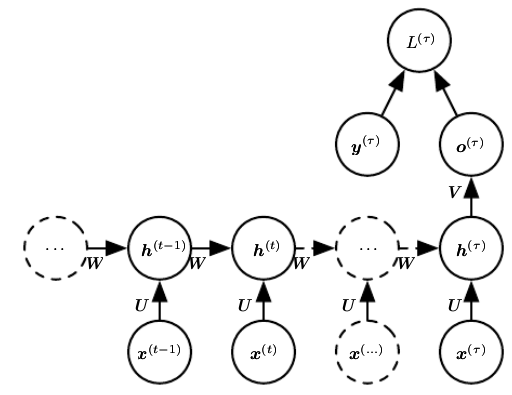
\includegraphics[scale=0.5]{imagenes/rnn3.png}
	\caption{Red recurrente que produce una única salida con conexiones entre las unidades ocultas.}
	\label{img:red-recurrente3}
\end{figure}

Como podemos ver, en este caso tenemos que los pesos se comparten sólo en la capa oculta. Esta red va almacenando conocimiento hasta llegar al último paso temporal, en el cual se emplea lo obtenido de los instantes de tiempo anteriores para producir una única salida. Este tipo de redes pueden usarse por ejemplo para predecir el siguiente valor de una serie temporal conociendo los valores de los instantes de tiempo anteriores.

Estos ejemplos que hemos dado no son una taxonomía, si no una serie de modelos que podemos utilizar y empleamos como ejemplo. Cada problema tiene unos requerimientos y objetivos que queremos cumplir y debemos ajustar nuestra red al problema que tengamos en consideración.

Hemos hecho un breve repaso de la idea de las redes neuronales recurrentes. En nuestro caso de aplicación práctica hemos empleado capas LSTM o Long-Short Term Memory, por lo que vamos a repasar cómo funcionan estas capas de forma teórica.

Las capas LSTM entran dentro de un tipo de redes neuronales recurrentes llamadas redes recurrentes con puertas. La idea es que estas redes elaboran caminos entre las entradas, salidas y estados internos que permiten recordar información u olvidarla si ya no nos es útil. Veamos esto con un esquema de cómo funcionan las LSTM:

\begin{figure}[H]
	\centering
	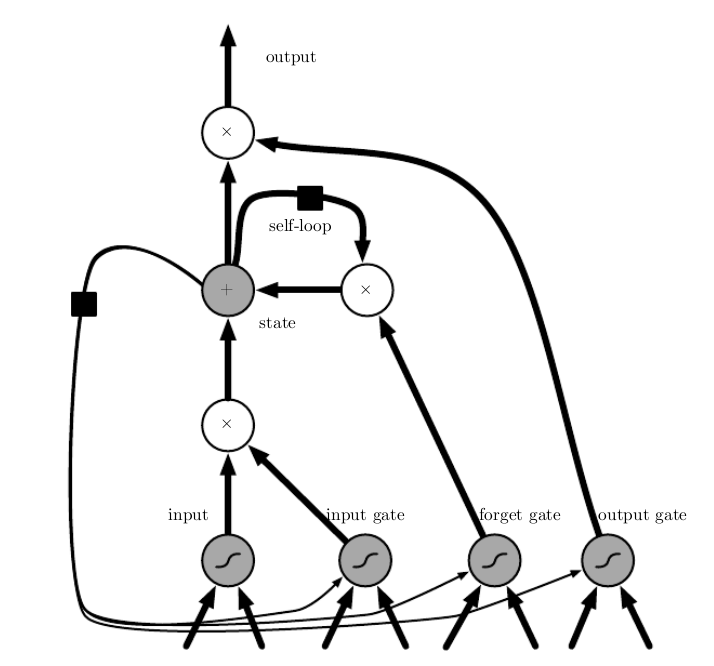
\includegraphics[scale=0.5]{imagenes/lstm.png}
	\caption{Esquema de funcionamiento de una celda LSTM.}
	\label{img:esquema-lstm}
\end{figure}

Estas celdas o neuronas están conectadas entre sí a través de los estados del sistema como en una red recurrente normal, por lo que cada uno de los estados tendría un peso y una conexión con la siguiente neurona. Podemos ver que la entrada se procesa con una neurona tradicional como teníamos en las capas densas, llegando esta entrada al estado de la celda y siendo acumulado o añadido si la función de activación y el resto de la celda lo permite. Podemos ver que el estado tiene un ciclo consigo mismo, moderado por la puerta de olvido. Esta puerta puede permitir olvidar el estado si se considera que es más beneficioso que conservarlo. El estado se realimenta de nuevo a la entrada tanto a la unidad de entrada, como a la de olvido y salida para poder tener su propio estado anterior como entrada del siguiente y decidir su acción. La neurona de salida puede cortar la salida producida por la celda.

Todo este esquema permite que la celda adquiera el estado de la anterior y lo integre como una entrada, procese su propia entrada basándose también en su estado anterior y decida si acumula el conocimiento, olvida o corta su salida en función de lo que mejor función de pérdida otorgue. Todo esto hace que nuestra celda pueda recordar todo el contenido de la serie temporal u olvidarlo en algún punto determinado u obviar una entrada si no se percibe de interés.

Este tipo de redes son actualmente muy exitosas en aplicación sobre texto, predicciones en series temporales y uso en vídeo para detección de trayectorias entre otros ejemplos. Nosotros las emplearemos en la parte práctica tanto solas como combinadas con convoluciones para obtener características algo mejores para alimentar la red.

\section{Autoencoders}

En la sección práctica veremos el uso de Autoencoders para la tarea de detección de anomalías que queremos desarrollar, por lo que necesitamos un poco de fundamento teórico para poder entender bien el funcionamiento de este tipo de arquitecturas.

El objetivo principal de estas arquitecturas es conseguir una codificación de los datos, es decir, una representación de los mismos en un espacio de menor dimensión que permita obtener suficiente información de ellos como para reconstruirlos a los originales cometiendo un error pequeño asumible. Esta arquitectura se puede ver dividida por tanto en dos partes, la función codificadora que codifica el dato y la función decodificadora que reconstruye el dato a partir de la codificación.

Normalmente no estamos interesados en la salida del Autoencoder, es decir en la decodificación del dato, si no en la codificación pero en nuestro caso estaremos interesados en la reconstrucción. Aunque nuestro objetivo sea obtener una salida final de calidad es fundamental fijarse en la codificación obtenida y que esta sea buena.

El tipo de Autoencoders que vamos a emplear son denominados como Autoencoders incompletos, ya que el objetivo es que la codificación sea de menor dimensión que la que poseen los datos originales. El proceso de aprendizaje de estos Autoencoders es sencillo: introducimos como entrada los datos originales y como salida predicha los mismos datos de entrada para que la red pueda aprender a reconstruirlos.

Para el proceso de detección de anomalías vamos a usar esta arquitectura del siguiente modo: entrenaremos con datos limpios sin anomalías e intentaremos que la reconstrucción sea lo más ajustada posible pero siempre con una codificación del menor tamaño posible para forzar la extracción de las características meramente esenciales. Tras esto lo que haremos será predecir, cuando obtengamos una reconstrucción con poco error estaremos ante un dato no anómalo o parecido a los no anómalos vistos previamente por la red y por tanto es capaz de reconstruirlos con poco error. Por contra si no es capaz de reconstruirlos bien y se comete mucho error estaremos ante un dato que no es normal y por tanto no ha sido visto por la red neuronal, cometiendo un mayor error de reconstrucción.

Veamos un ejemplo de un autoencoder de capas totalmente conectadas:

\begin{figure}[H]
	\centering
	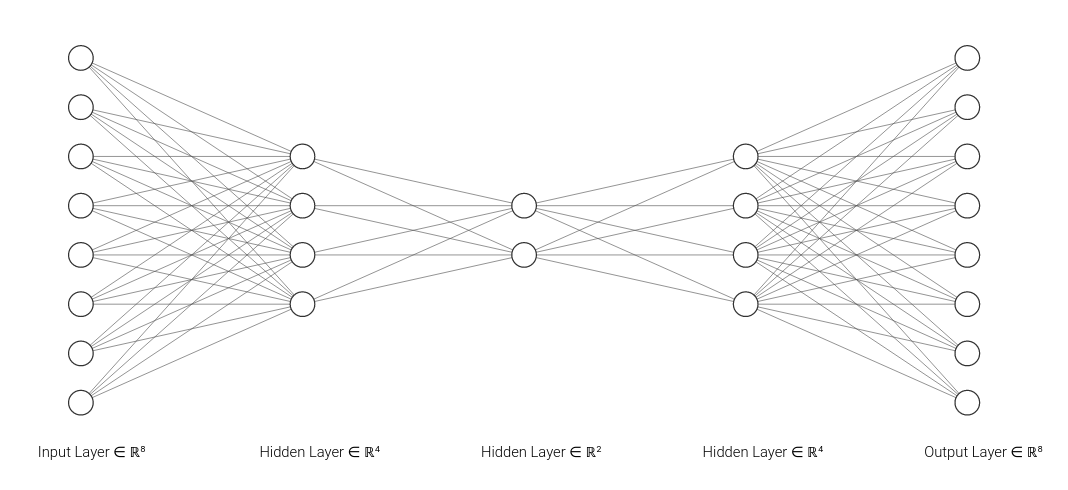
\includegraphics[scale=0.35]{imagenes/autoencoder_ejemplo.png}
	\caption{Ejemplo de Autoencoder con capas totalmente conectadas.}
	\label{img:ejemplo-autoencoder}
\end{figure}

Como podemos observar en la figura \ref{img:ejemplo-autoencoder} tenemos datos de entrada con 8 variables, reducimos primero la dimensión a 4 y finalmente la codificación reduce la dimensión a dos variables. Tras esto viene la decodificación que devuelve los datos primero a 4 variables y finalmente a las 8 iniciales.

Esta misma arquitectura se puede emplear con varias capas distintas, en la práctica nosotros emplearemos capas densas y capas LSTM para extraer una codificación de menor dimensionalidad que la original.
%
\part{Modelos implementados y análisis de resultados}
\label{part:explicacionmodelos_analisisrresultados}

\chapter{Modelos implementados}
\label{chapter:modelos}

En este capítulo vamos a repasar los modelos implementados que analizaremos. La implementación de todos estos modelos se ha hecho de forma propia en Python empleando el framework Keras para la construcción de las redes neuronales sobre Tensorflow en su versión 2.

La implementación de todos estos modelos es libre y se puede consultar en el repositorio Deep Learning Outlier Detection o DLOD \href{https://github.com/nacheteam/DLOD}{(link)}.

Para el uso práctico en esta cuestión se han implementado dos tipos de modelos: autoencoders y modelos predictivos. Vamos a repasar brevemente cómo emplearemos estos modelos para la detección de anomalías.

En primer lugar tenemos los modelos Autoencoders, de los que acabamos de hacer un repaso en el capítulo anterior. Los modelos implementados siempre intentan reducir la dimensión para luego reconstruir los datos. Cuando hacemos este paso a un espacio de menor dimensión, estamos intentando reducir las características de nuestras instancias al menor número posible de ellas que las explica lo mejor posible. Nuestra intención al hacer esto es que, las características con las que nos quedamos explican la mayoría de los datos o lo que es lo mismo, los datos normales. Estas características de la reducción de dimensionalidad no van a ser capaces de explicar los datos anómalos y por tanto el error de reconstrucción para los datos anómalos será mayor que el error de reconstrucción para los normales, por lo que podemos usar esta métrica como puntuación o score de anomalía.

En segundo lugar se han implementado modelos de predicción. Estos modelos son entrenados para predecir las secuencias o instancias de datos normales, por lo que aprendemos la distribución subyacente a los datos no anómalos. Cuando intentemos predecir una nueva secuencia de datos normales cometeremos poco error, porque hemos enseñado a nuestra red a que prediga las secuencias normales. Por contra, cuando nos encontremos con datos anómalos, el predictor no tendrá la distribución subyacente de dichos datos y por tanto cometerá mucho más error en la predicción. Teniendo esto podemos usar como métrica o score de anomalía la diferencia entre el dato real y el predicho: a mayor diferencia más anómalo y a menor diferencia menos anómalo.

\section{Autoencoder totalmente conectado}

La primera aproximación lógica sin tener en cuenta el tipo de dato con el que tratamos es un autoencoder con capas densas o totalmente conectadas. El objetivo de este Autoencoder es reconstruir instancia por instancia sin tener en cuenta ningún tipo de temporalidad, como si fuesen datos estáticos. 

Es claro que este tipo de modelos no aprovechan la estructura y dependencia de los datos, pero debemos empezar por algún sitio a probar.

La arquitectura de estos modelos ya ha sido puesta como ejemplo en las secciones anteriores, por lo que no hay mucho más que añadir sobre la misma. En un principio la arquitectura de Autoencoder no tiene por qué ser simétrica, es decir, no tiene por qué ser igual la reducción desde los datos originales al encoding que desde el encoding a la reconstrucción. En el caso que contemplamos se ha utilizado una estructura simétrica, pues es la más empleada y descrita en la literatura.

Para entrenar el autoencoder debemos entrenarlo con datos en condiciones normales para que aprenda bien la distribución subyacente de dichos datos, pues es lo que nos interesa para que el error de reconstrucción sea bajo en los datos normales y alto en los anómalos. En el conjunto de datos del que disponemos, los operarios etiquetan los mantenimientos de la máquina y las alarmas de la misma. Un mantenimiento es precedido por alarmas que no precisan de una parada completa de la misma, mientras que un mantenimiento es un fallo de mayor gravedad que sí requiere de una parada completa para ser solucionado. Este tipo de mantenimientos son los que nos interesan, pero las alarmas nos pueden alertar con anticipación de la ocurrencia de un mantenimiento. Por ello para entrenar el autoencoder se eliminan los datos de mantenimiento y de alarmas, para entrenar siempre la red con datos en condiciones normales.

Para tener un poco más clara la estructura de estas redes vamos a poner un esquema de ejemplo de un posible autoencoder con las dimensiones reales de los datos:

\begin{figure}[H]
	\centering
	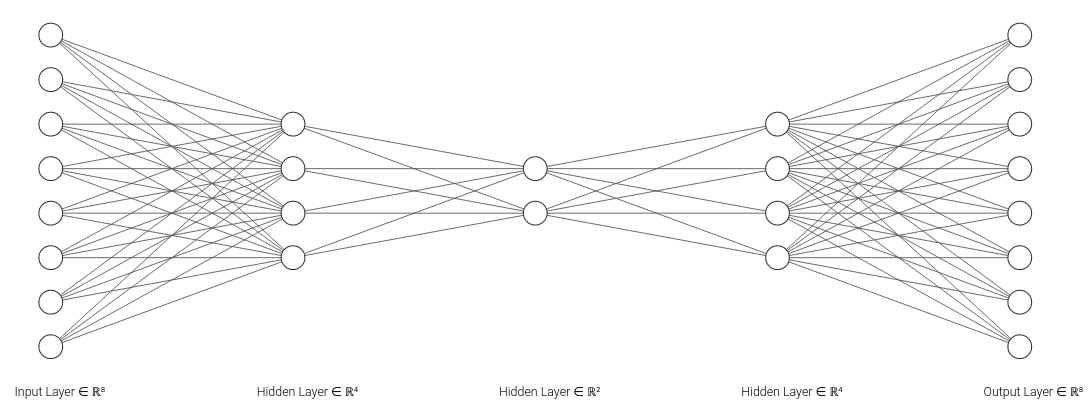
\includegraphics[scale=0.35]{imagenes/autoencoder-fcc.png}
	\caption{Ejemplo de una arquitectura simétrica de autoencoder no completo para detección de anomalías.}
	\label{img:autoencoder-fcc}
\end{figure}

En nuestro caso los datos parten de dimensión 106 (tienen 106 variables numéricas originalmente) y se reducen a 64, 32, y finalmente a 16 características, por lo que se reducen más de 7 veces con respecto a su tamaño original.

Finalmente vamos a ver el código que genera el modelo en Python para terminar esta sección:

\begin{lstlisting}[language=Python]
def buildAutoencoder(self):	
	encoding_dim=self.hidden_neurons[-1]
	
	input_layer = layers.Input(shape=self.input_dim)
	encoder = layers.Dense(self.hidden_neurons[0], activation=self.hidden_activation, activity_regularizer = l2(self.l2_regularizer))(input_layer)
	encoder = layers.Dropout(self.dropout)(encoder)
	
	for neuron in self.hidden_neurons[1:]:
		encoder = layers.Dense(neuron, activation=self.hidden_activation, activity_regularizer = l2(self.l2_regularizer))(encoder)
		encoder = layers.Dropout(self.dropout)(encoder)
	
	reverse_layers = self.hidden_neurons[::-1][1:]
	
	decoder = layers.Dense(reverse_layers[0], activation=self.hidden_activation, activity_regularizer = l2(self.l2_regularizer))(encoder)
	decoder = layers.Dropout(self.dropout)(decoder)
	
	for neuron in reverse_layers[1:]:
		decoder = layers.Dense(neuron, activation=self.hidden_activation, activity_regularizer = l2(self.l2_regularizer))(decoder)
		decoder = layers.Dropout(self.dropout)(decoder)
	
	decoder = layers.Dense(self.input_dim[0], activation=self.output_activation, activity_regularizer = l2(self.l2_regularizer))(decoder)
	
	autoencoder = Model(input_layer, decoder)
	autoencoder.compile(optimizer=self.optimizer, loss=self.loss)
	
	return autoencoder
\end{lstlisting}

Cabe decir que esta función está encapsulada dentro de una clase que se encarga de generar la estructura en base a unos parámetros, entrenarla con los datos que le demos al modelo y predecir y sacar la puntuación de anomalía para cada una de las instancias del conjunto de test.

\section{Autoencoder totalmente conectado por lotes}

En la sección anterior hemos comentado que el primero paso natural al hacer un autoencoder para detección de anomalías es empezar por la arquitectura más sencilla posible: la totalmente conectada. También hemos comentado que esta arquitectura no aprende ni usa la dependencia temporal de los datos presente por ser estos una serie temporal, por tanto es una herramienta de poco potencial para este tipo de datos.

Las capas totalmente conectadas también nos pueden valer para procesar lotes de datos, es decir, bloques de datos sin saltos temporales. De esta forma, podemos hacer que una arquitectura sencilla pueda aprender algo más sobre la dependencia temporal de los datos. Si lo pensamos, lo que estamos haciendo para poder procesar lotes, es tomar $n$ datos juntos y colocarlos en formato columna uno detrás de otro, por lo que nuestro objetivo final ya no será la reconstrucción de una instancia, si no la reconstrucción de un lote completo.

Esto es una aproximación un poco mejor que la anterior, pues ahora ya tenemos datos completos y podemos procesar y aprender la distribución subyacente pero por supuesto no es tan potente como las capas que hemos estudiado en la parte teórica.

En este caso, para que tengamos solo una puntuación por instancia, hemos reconstruido lotes sin solapamiento. Es decir, procesamos las primeras $n$ instancias, luego desde la $n+1$ hasta la $2n$ etcétera. Con esto no tenemos que hacer ponderaciones de las puntuaciones al obtener sólo una por instancia ya que los lotes no contienen datos repetidos.

El esquema de esta arquitectura empieza con un lote de datos en formato matriz, que reconvertimos a un vector colocando una fila detrás de la siguiente. Tras esta conversión de tamaños tenemos la misma arquitectura que en la sección anterior siendo el final la operación inversa de vector a matriz.

\begin{figure}[H]
	\centering
	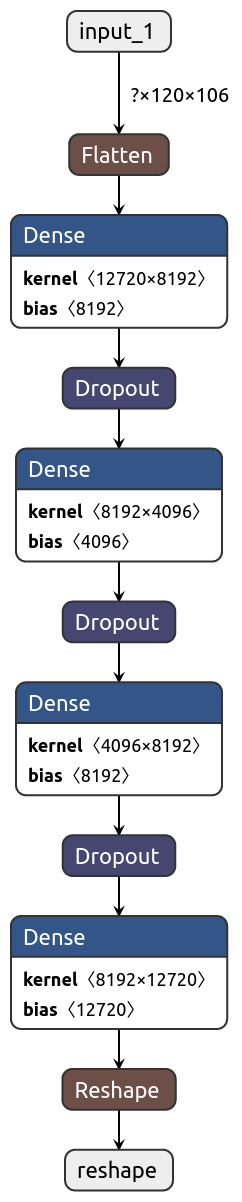
\includegraphics[scale=0.4]{imagenes/autoencoder-fcc-batch.png}
	\caption{Ejemplo de una arquitectura de Autoencoder de reconstrucción por lotes.}
	\label{img:autoencoder-fcc-batch}
\end{figure}

Como podemos ver en la arquitectura, se recibe una matriz de 120 instancias de 106 atributos cada una de ellas y lo primero que hacemos con ella es aplanarla como hemos comentado. Tras esto viene toda la arquitectura normal de un autoencoder no completo para finalizar con un reshape que nos devuelve la salida a un formato matricial.

\begin{lstlisting}[language=Python]
def buildAutoencoder(self):
	encoding_dim=self.hidden_neurons[-1]
	
	input_layer = layers.Input(shape=(self.instance_batch, self.num_features))
	flatten = layers.Flatten()(input_layer)
	encoder = layers.Dense(self.hidden_neurons[0], activation=self.hidden_activation, activity_regularizer = l2(self.l2_regularizer))(flatten)
	encoder = layers.Dropout(self.dropout)(encoder)
	
	for neuron in self.hidden_neurons[1:]:
		encoder = layers.Dense(neuron, activation=self.hidden_activation, activity_regularizer = l2(self.l2_regularizer))(encoder)
		encoder = layers.Dropout(self.dropout)(encoder)
	
	reverse_layers = self.hidden_neurons[::-1][1:]
	
	decoder = layers.Dense(reverse_layers[0], activation=self.hidden_activation, activity_regularizer = l2(self.l2_regularizer))(encoder)
	decoder = layers.Dropout(self.dropout)(decoder)
	
	for neuron in reverse_layers[1:]:
		decoder = layers.Dense(neuron, activation=self.hidden_activation, activity_regularizer = l2(self.l2_regularizer))(decoder)
		decoder = layers.Dropout(self.dropout)(decoder)
	
	decoder = layers.Dense(self.instance_batch * self.num_features, activation=self.output_activation, activity_regularizer = l2(self.l2_regularizer))(decoder)
	reshape = layers.Reshape(target_shape=(self.instance_batch, self.num_features))(decoder)
	
	autoencoder = Model(input_layer, reshape)
	autoencoder.compile(optimizer=self.optimizer, loss=self.loss)
	
	return autoencoder
\end{lstlisting}

\section{Autoencoder LSTM}

La siguiente arquitectura que se ha desarrollado es la última que toma como estructura la de codificación-reconstrucción. En este caso, para poder aprovechar al máximo la dependencia temporal y aplicando lo que hemos visto en la sección de teoría, se ha desarrollado un Autoencoder con capas LSTM. En este caso, como ya hemos visto, las capas LSTM aprovechan la dependencia temporal ya que tienen un estado interno que les permite almacenar información de las instancias anteriores y poder olvidarlo cuando sea necesario.

En este modelo de red podemos construirlo de distintas formas. En primer lugar podemos pensar en un modelo mixto que tenga una primera capa LSTM y luego haga la codificación con las características obtenidas de la capa LSTM a través de capas totalmente conectadas. La otra opción es que hagamos un Autoencoder sólo con capas LSTM, este es el tipo de modelo que se ha elegido. 

La elección de un Autoencoder de capas LSTM únicamente responde a la capacidad de olvidar información que tienen estas capas. Si sólo fuese interesante sacar dependencias temporales en las primeras capas las siguientes estarían activando el olvido y el bloqueo de entrada-salida para forzar a que su funcionamiento sea como el de una capa totalmente conectada con estados internos intermedios. Este razonamiento es el que nos lleva a confiar en la capacidad y potencia de estas capas para elaborar un Autoencoder sólo con ellas.

\begin{figure}[H]
	\centering
	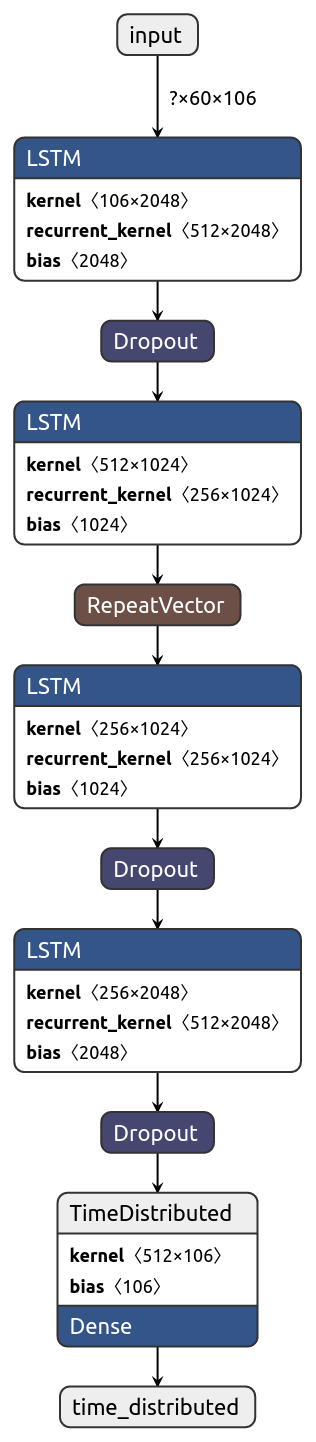
\includegraphics[scale=0.4]{imagenes/autoencoder-lstm.png}
	\caption{Ejemplo de una arquitectura de Autoencoder LSTM.}
	\label{img:autoencoder-lstm}
\end{figure}

Como podemos ver, el modelo de Autoencoder con capas LSTM puede tener varias capas hasta el encoding y respeta la simetría que hemos comentado antes. La programación de este tipo de redes es un poco compleja, pues tenemos que tener en cuanta cuándo tenemos que devolver secuencias de datos y cuándo vectores para que las salidas de una capa encajen con las entradas que espera la siguiente capa.

Para esta arquitectura de red estamos introduciendo un lote de datos, como en el caso de la sección anterior una matriz con varias instancias de datos. Cuando vamos pasando de una capa a otra tenemos que devolver secuencias, pues es lo que las capas LSTM esperan, pero cuando llegamos al encoding queremos obtener un vector como en los otros modelos de encoding. Es por esto que tenemos que repetir ese vector de encoding para poder hacer de nuevo la subida o decoding hacia la reconstrucción de los datos, pues de otra forma no recibirían una secuencia.

Veamos por último el código Python que genera este tipo de modelos:

\begin{lstlisting}[language=Python]
def buildAutoencoder(self):
	autoencoder = Sequential()
	autoencoder.add(layers.InputLayer(input_shape = (self.instance_batch, self.num_features)))
	for neurons in self.hidden_neurons[:-1]:
		autoencoder.add(layers.LSTM(units=neurons,
		activation=self.hidden_activation,
		recurrent_activation=self.recurrent_activation,
		activity_regularizer=l2(self.l2_regularizer),
		recurrent_dropout=self.recurrent_dropout,
		return_sequences=True))
		autoencoder.add(layers.Dropout(self.dropout))
	autoencoder.add(layers.LSTM(units=self.hidden_neurons[-1],
	activation=self.hidden_activation,
	recurrent_activation=self.recurrent_activation,
	activity_regularizer=l2(self.l2_regularizer),
	recurrent_dropout=self.recurrent_dropout,
	return_sequences=False))
	autoencoder.add(layers.RepeatVector(n=self.instance_batch))
	for neurons in self.hidden_neurons[::-1]:
		autoencoder.add(layers.LSTM(units=neurons,
		activation=self.hidden_activation,
		recurrent_activation=self.recurrent_activation,
		activity_regularizer=l2(self.l2_regularizer),
		recurrent_dropout=self.recurrent_dropout,
		return_sequences=True))
		autoencoder.add(layers.Dropout(self.dropout))
	autoencoder.add(layers.TimeDistributed(layers.Dense(units=self.num_features)))
	autoencoder.compile(optimizer=self.optimizer, loss=self.loss)
return autoencoder
\end{lstlisting}

\section{Modelo de predicción LSTM}

Este modelo entra dentro del segundo tipo de modelos implementados: los de predicción. La intención de estos modelos es aprender a predecir muy bien las instancias en momentos de comportamiento normal de la máquina, de esta forma cuando estemos ante datos normales tendremos un error de predicción muy pequeño y cuando estemos ante datos anómalos con los que no se ha entrenado el error será mayor.

Para esta arquitectura se han empleado de nuevo capas LSTM. Con estas capas podemos obtener dependencias temporales de los datos, por lo que el modelo lo que va a hacer es tomar lotes de $n$ datos y predecir los $m$ siguientes. Este número $m$ puede ser uno o puede ser mayor que uno, es decir, con un lote podemos predecir uno o más datos siguientes. En este estudio se ha considerado que la mejor elección y la más precisa es la de predicción punto a punto, es decir, tomamos un lote y predecimos el siguiente punto, desplazamos el lote un instante de tiempo y volvemos a predecir la siguiente instancia. De esta forma lo que tenemos es una única predicción de cada instancia y predecimos solo un dato por cada lote que tenemos. El código desarrollado está preparado para soportar más de una predicción si se considerase necesario.

Debemos tener en cuenta que hacer esta operación de entrenamiento es altamente costosa pues, para poder predecir cada una de las instancias de un conjunto de 40 millones de datos aproximadamente, necesitamos almacenar en memoria $40 \ millones \cdot n$. Si consideramos por ejemplo lotes de 60 instancias o lo que es lo mismo un minuto de datos, tenemos que almacenar en memoria 240 millones de instancias lo cual no es posible. Por ello cabe detenerse un momento en explicar la solución técnica que se ha adoptado para solventar este contratiempo.

Cuando queremos entrenar una red con una serie temporal de un gran tamaño Keras tiene como herramienta la clase TimeSeriesGenerator, que nos permite hacer lotes de series temporales con lo que queremos que entrene y el objetivo al que queremos que llegue. Esta herramienta actualmente tiene un problema, pues sólo permite el uso para predicción con el siguiente punto y no con varias instancias por lote. Aunque para este experimento no se ha empleado esto se ha generalizado el funcionamiento de la clase TimeSeriesGenerator de Keras para que pueda devolver varias instancias por cada lote.

Veamos ahora la estructura de este tipo de redes:

\begin{figure}[H]
	\centering
	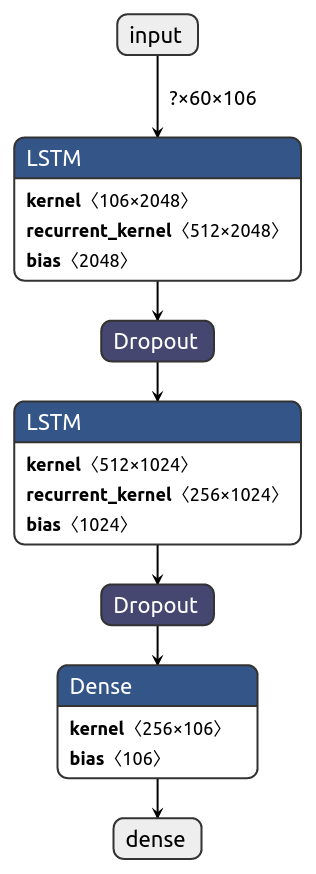
\includegraphics[scale=0.4]{imagenes/lstm-forecaster.png}
	\caption{Ejemplo de una arquitectura de predictor LSTM con una única instancia en la predicción.}
	\label{img:forecaster-lstm}
\end{figure}

Como podemos ver, en este ejemplo tenemos dos capas LSTM y una capa final totalmente conectada. Las capas LSTM nos sirven para poder obtener las dependencias temporales que tenemos intrínsecas por ser series temporales. Estas características son pasadas a una última capa totalmente conectada que nos sirve para igualar la dimensión a la que queramos. En esta red estamos prediciendo una única instancia por batch, pero como es lógico la arquitectura variaría ligeramente, vamos a ver un ejemplo de cómo sería la arquitectura de la red si quisiéramos predecir más de una instancia:

\begin{figure}[H]
	\centering
	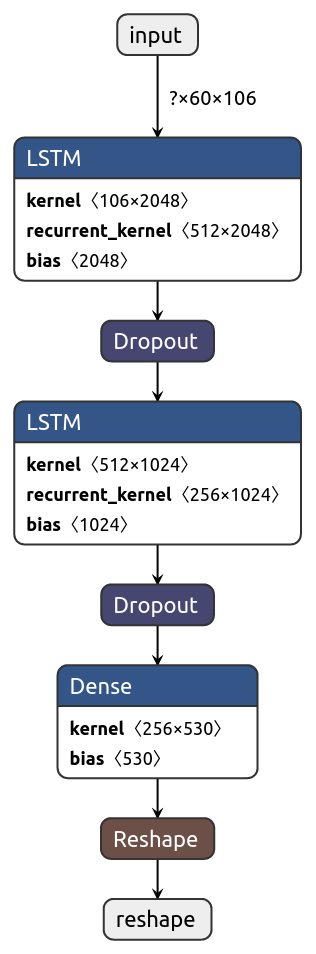
\includegraphics[scale=0.4]{imagenes/lstm-forecaster2.png}
	\caption{Ejemplo de una arquitectura de predictor LSTM con 5 instancias en la predicción.}
	\label{img:forecaster-lstm2}
\end{figure}

Como podemos ver la capa totalmente conectada del final ahora tiene como tamaño la dimensión de los datos por el número de instancias que queremos predecir, por lo que la capa siguiente es una capa de reajuste de los datos que nos los convierte a una matriz en la que cada fila es una de las instancias predichas, yendo estas en orden. Esto quiere decir que la primera fila está temporalmente antes que la segunda y así sucesivamente.

Lo último que queda por añadir es que para entrenar todos estos modelos con secuencias de datos, nos tenemos que asegurar que no son secuencias cortadas. Al eliminar los datos anómalos como las alarmas y los mantenimientos se nos quedan huecos temporales en los datos. Estos huecos pueden producir que haya secuencias con saltos temporales, lo cual no es deseable así que tenemos que eliminar las secuencias que contengan alguno de estos saltos temporales.

Finalmente este es el código que genera este tipo de arquitecturas:

\begin{lstlisting}[language=Python]
def buildForecaster(self):
	model = Sequential()
	model.add(layers.InputLayer(input_shape = (self.instance_batch, self.num_features)))
	for neurons in self.hidden_neurons[:-1]:
		model.add(layers.LSTM(units=neurons,
		activation=self.hidden_activation,
		recurrent_activation=self.recurrent_activation,
		activity_regularizer=l2(self.l2_regularizer),
		recurrent_dropout=self.recurrent_dropout,
		return_sequences=True))
		model.add(layers.Dropout(self.dropout))
	model.add(layers.LSTM(units=self.hidden_neurons[-1],
	activation=self.hidden_activation,
	recurrent_activation=self.recurrent_activation,
	activity_regularizer=l2(self.l2_regularizer),
	recurrent_dropout=self.recurrent_dropout,
	return_sequences=False))
	model.add(layers.Dropout(self.dropout))
	model.add(layers.Dense(self.num_features*self.npred, activation=self.output_activation, activity_regularizer = l2(self.l2_regularizer)))
	if self.npred>1:
		model.add(layers.Reshape(target_shape=(self.npred, self.num_features)))
	model.compile(optimizer=self.optimizer, loss=self.loss)
	return model
\end{lstlisting}

\section{Modelo de predicción CNN-LSTM}

El último modelo implementado es otro modelo de predicción como el se la sección anterior, pero ahora empleamos capas convolucionales para intentar extraer características más relevantes de los datos sin romper la temporalidad de los mismos antes de pasarlos por las capas LSTM.

Lo primero que vamos a hacer con la entrada es pasarla por capas convolucionales 1D. En la sección de teoría estudiamos el comportamiento de estas capas, introduciendo primero la operación de convolución en una dimensión y luego en dos dimensiones. Cuando aplicamos la operación de convolución en dos dimensiones, para que sea útil e interesante, tenemos que tener datos que estén correlados o que tengan dependencias en ambas dimensiones. Si pensamos por ejemplo en una imagen, es claro que la información de un píxel está condicionada por la de los píxeles que tiene a su alrededor. En el caso que tenemos nosotros no es así. Tenemos una matriz cuyas filas son cada una de las instancias consideradas y las columnas son las características de dichas instancias. Es claro que tenemos una dependencia en el eje Y, es decir entre las filas, pues las instancias están consecutivas en el tiempo y cada una de ellas está condicionada por las anteriores y condiciona las siguientes. Por contra, en las columnas, no tenemos esa dependencia. A priori las características no tienen ningún tipo de dependencia entre sí ni correlación, pues no se han ordenado para ello ni tendría por qué existir dicha correlación entre las variables si tenemos un conjunto de datos óptimo.

Con esto dicho por tanto está claro el eje en el que tiene sentido hacer la convolución: el eje de las filas. Este tipo de operación de convolución uno dimensional está soportada por Keras mediante la capa Conv1D. Tras pasar los datos por varias convoluciones y agregaciones se pasan por capas LSTM, de forma que con las nuevas características obtenidas por la convolución las capas LSTM pueden trabajar algo mejor. Finalmente la arquitectura de la red termina con una serie de capas totalmente conectadas que igualan la dimensión con la que nosotros queramos para predecir una o más instancias.

Estos modelos son ampliamente empleados en predicción por su buen desempeño como se puede ver en los artículos \cite{lih_oh_automated_2018} y \cite{tae_young_predicting_2019} que han servido para obtener una arquitectura de red adecuada para nuestro problema.

En cuanto al entrenamiento y predicción este modelo es muy similar al anterior. Vamos a entrenarlo con secuencias de datos y vamos a predecir una única instancia, aunque el modelo está preparado en su implementación para poder predecir más de una por cada lote. Además, nos aseguramos también de que el modelo no se entrena con secuencias de datos con saltos temporales. De igual forma es necesario emplear la clase TimeSeriesGenerator modificada para poder manejar los datos de entrenamiento, pues al predecir una instancia por lote tenemos muchos más datos que los originales.

Veamos un esquema de este tipo de arquitectura:

\begin{figure}[H]
	\centering
	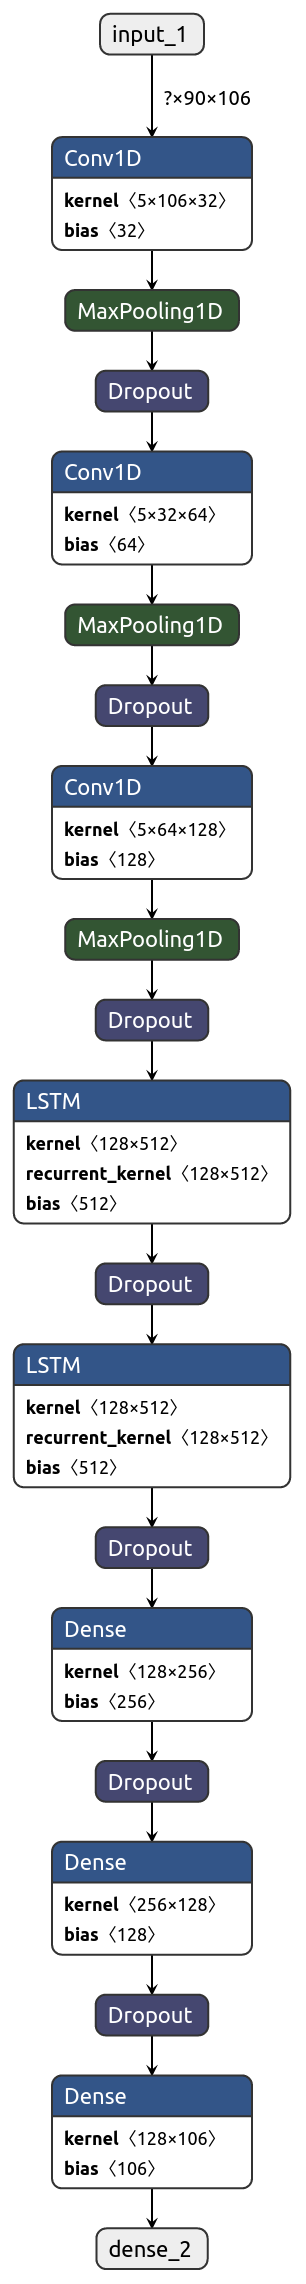
\includegraphics[scale=0.28]{imagenes/cnn-lstm-forecaster.png}
	\caption{Ejemplo de una arquitectura de predictor CNN-LSTM.}
	\label{img:cnn-lstm-forecaster}
\end{figure}

Como podemos ver en este ejemplo tenemos tres capas de convolución con 3 agregaciones con el máximo, tras esto dos capas LSTM y finalmente otras dos capas totalmente conectadas que hacen que la dimensión final sea la de una instancia, por lo que este ejemplo en concreto predice una única instancia. Si quisiéramos predecir más de una tendríamos que hacer lo mismo que en el modelo anterior, añadiendo un reshape.

Por último veamos el código Python que genera el modelo:

\begin{lstlisting}[language=Python]
def buildForecaster(self):
	input = layers.Input(shape = (self.instance_batch, self.num_features))
	
	conv = layers.Conv1D(filters=self.conv_filters[0], kernel_size = self.kernel_size,
	activation=self.conv_activation)(input)
	conv = layers.MaxPooling1D(self.pooling_size)(conv)
	conv = layers.Dropout(self.dropout)(conv)
	for nfilters in self.conv_filters[1:]:
		conv = layers.Conv1D(filters=nfilters, kernel_size = self.kernel_size,
		activation=self.conv_activation)(conv)
		conv = layers.MaxPooling1D(self.pooling_size)(conv)
		conv = layers.Dropout(self.dropout)(conv)
	
	lstm=None
	first_lstm=True
	for neurons in self.lstm_neurons[1:]:
		if first_lstm:
			lstm = layers.LSTM(units=neurons,
			activation=self.lstm_activation,
			recurrent_activation=self.recurrent_activation,
			activity_regularizer=l2(self.l2_regularizer),
			recurrent_dropout = self.recurrent_dropout,
			return_sequences=True)(conv)
			lstm = layers.Dropout(self.dropout)(lstm)
			first_lstm=False
		else:
			lstm = layers.LSTM(units=neurons,
			activation=self.lstm_activation,
			recurrent_activation=self.recurrent_activation,
			activity_regularizer=l2(self.l2_regularizer),
			recurrent_dropout = self.recurrent_dropout,
			return_sequences=True)(lstm)
			lstm = layers.Dropout(self.dropout)(lstm)
	lstm = layers.LSTM(units=neurons,
	activation=self.lstm_activation,
	recurrent_activation=self.recurrent_activation,
	activity_regularizer=l2(self.l2_regularizer),
	recurrent_dropout = self.recurrent_dropout,
	return_sequences=False)(lstm)
	lstm = layers.Dropout(self.dropout)(lstm)
	
	dense=None
	if len(self.dense_neurons)>1:
		dense = layers.Dense(units=self.dense_neurons[0], activation=self.dense_activation)(lstm)
		dense = layers.Dropout(self.dropout)(dense)
	for neurons in self.dense_neurons[1:]:
		dense = layers.Dense(units=neurons, activation=self.dense_activation)(dense)
		dense = layers.Dropout(self.dropout)(dense)
	
	if len(self.dense_neurons)==0:
		dense = layers.Dense(units=self.num_features, activation=self.output_activation)(lstm)
	else:
		dense = layers.Dense(units=self.num_features, activation=self.output_activation)(dense)
	
	model = Model(inputs=input, outputs=dense)
	model.compile(optimizer=self.optimizer, loss=self.loss)
	return model
\end{lstlisting}
%
\chapter{Algoritmo de detección de anomalías}
\label{chapter:algoritmo-anomalias}

El capítulo anterior ha tratado sobre los modelos que se han implementado. Estos algoritmos lo que hacen es tomar unos datos normales como entrada, entrenar y luego evaluar unos datos de test. Tras evaluar los datos de test lo que tenemos son scores de anomalías, es decir, para cada instancia del conjunto de test tenemos una puntuación. Con esta puntuación por sí sola no tenemos ningún tipo de detección, lo que tenemos que hacer es utilizar estas puntuaciones para alimentar algún algoritmo que detecte los eventos anómalos.

Cuando estemos ante eventos normales tendremos puntuaciones bajas, mientras que si estamos ante eventos anómalos tendremos puntuaciones más altas. En este sentido podemos pensar en las puntuaciones como en una serie temporal uno dimensional, en la que queremos hallar los puntos en los que destaca por la subida en el score por encima de los niveles normales.

Para esto lo primero que vamos a hacer es pasar los datos de tipo numérico a categórico, es decir, cuándo tenemos una anomalía y cuando estamos ante un dato normal. Para ello se ha elaborado un sistema de cotas que permite establecer un punto a partir del cual dejamos de considerar dicho dato como normal y lo empezamos a considerar anómalo.

El sistema basa su comportamiento en dos cotas, una cota general y otra cota local. La cota general es pasada como un parámetro externo, en nuestro caso hemos reservado unos cuantos días para calcular la cota global de forma que no empleemos los datos de test para esto. La cota general puede ser calculada de muchas formas, en nuestro caso se han probado la media de las puntuaciones, la media mas tres desviaciones típicas, la mediana, el percentil 95 y la mediana mas tres desviaciones típicas. De esta forma la metodología seguida es, reservamos de los 468 días en total de nuestro conjunto de datos los primeros días para entrenamiento de las redes neuronales, dejando los dos últimos meses para cálculo de cotas y el conjunto de test. De estos dos últimos meses el primero de ellos será para cálculo de cotas y el segundo como test. Esto nos deja aproximadamente dos millones y medio de instancias de test.

Una vez dicho esto, lo primero que vamos a describir es el algoritmo que convierte los scores en clases. Vamos a ir pasando una ventana deslizante por los datos de un tiempo definido previamente, en este caso 3 horas de datos. Esta ventana la vamos a dividir en dos partes, la primera va a ser para calcular una cota local, para lo cual emplearemos la media mas 3 desviaciones típicas. Esta cota local se va a combinar con la cota global haciendo una media. La intención de esta cota cambiante es que podamos ajustarnos un poco mejor a los datos que tenemos, si tenemos unos datos muy anómalos y estos persisten mucho tiempo, puede que haya un cambio de concepto en las puntuaciones de anomalía. Por otro lado la cota global introducida nos da un mínimo que deben cumplir nuestras puntuaciones para ser consideradas anómalas y mantiene el algoritmo estable.

Ya tenemos la cota total, generada a partir de la cota global y la cota local. Tras estos datos que hemos empleado para el cálculo de la cota local, vamos a emplear dicha cota para ver si los puntos la sobrepasan o no. En caso de que la sobrepasen marcamos los puntos con un uno, en caso contrario con un cero. De esta forma, al final del proceso, vamos a tener los puntos etiquetados como anómalos o normales en función del comportamiento que tienen local y globalmente con respecto a su puntuación.

Una vez que tenemos los puntos etiquetados como anómalos o normales, tenemos que determinar cuándo un periodo de tiempo es anómalo o no. Pensemos de la siguiente forma: tenemos los datos de un día completo ya etiquetados con ceros y unos en función de si las instancias son normales o anómalas. Teniendo esto podemos pasar una ventana deslizante por estos datos e ir viendo si tenemos suficientes puntos dentro anómalos como para considerar esta ventana deslizante anómala o no. 

Haciendo esto lo que vamos a tener al final es un conjunto de ventanas que consideramos anómalas y por tanto daríamos la alarma a los operarios si nos encontrásemos en una de estas ventanas deslizantes. Lo siguiente que necesitamos saber es cuándo vamos a considerar que lo estamos haciendo bien y cuándo lo estamos haciendo mal, es decir, cuando tenemos un verdadero positivo y cuándo tenemos un falso positivo. 

Desde la empresa, se nos dijo que lo más interesante era intentar predecir un mantenimiento en la franja temporal previa al mismo. En concreto se nos trasladó que lo más lógico es que no fuese ni mucho tiempo ni poco tiempo para que se pudiera asociar a algo concreto y que no fuese demasiado tarde para arreglarlo. Por ello se fijó que tendríamos un verdadero positivo si obteníamos una ventana anómala en la franja de 6 horas previas a un mantenimiento. Si tenemos una alerta en cualquier momento previo a dicha franja tendremos por tanto un falso positivo.

Por otro lado debemos decidir el número de datos que queremos procesar en estas ventanas deslizantes. Tiene que ser un número suficiente como para analizar el comportamiento local pero que no sea demasiado pequeña, ya que no obtendríamos demasiada información. Se decidió que ventanas deslizantes de dos horas con solapamiento de una hora era un tamaño interesante y válido para este fin.

Por tanto ya tenemos el tamaño de la ventana deslizante, el solapamiento y cuándo consideramos que tenemos un falso positivo y un verdadero positivo. Ahora nos falta decidir cuándo vamos a decir que tenemos una ventana anómala y por tanto debemos dar la alarma. En este caso se decidió que un porcentaje razonable de anomalías era un cinco por ciento. Esto quiere decir que si tenemos menos de un 5\% de anomalías en nuestra ventana no vamos a dar la alarma, pero si superamos o igualamos este porcentaje entonces marcaremos dicha ventana como anómala.

Con todos estos parámetros ya tenemos todo lo que necesitamos. Vamos a ir deslizando una ventana de dos horas con solapamiento de una hora, si en dicha ventana se supera el 5\% de anomalías entonces marcamos la ventana. Si esta ventana se encuentra dentro del intervalo de seis horas previas a un mantenimiento estamos ante un verdadero positivo, si no se encuentra en esta franja temporal estamos ante un falso positivo.

Con esto dicho podemos sacar tres métricas importantes e interesantes para nuestro problema: los verdaderos positivos, los falsos positivos y los mantenimientos que detectamos sobre el total presentes en el conjunto de test. Con esto hemos convertido un problema no supervisado, con etiquetas poco concretas en un problema más definido sobre el que podemos sacar algunas métricas.

Como añadido a todo esto, se añade la posibilidad de eliminar las anomalías puntuales que más nos puedan alterar la clasificación de las mismas en normales o anómalas. Por ello se añade como parámetro para probar el saturar las puntuaciones de anomalías que superen el percentil 99, cambiándolas por la mediana del score del resto de datos. Esto es un parámetro más a probar por lo que se ha estudiado todo el sistema haciendo esta saturación y sin hacerla.
%
\chapter{Experimentación y Resultados}
\label{chapter:experimentacion-resultados}

\section{Algoritmos empleados en la comparativa y parámetros empleados}

En todas las secciones anteriores hemos descrito el funcionamiento de nuestro sistema de detección de anomalías y alarmas. Como hemos podido comprobar, este sistema es como un puzle en el que tenemos tres piezas: el algoritmo de obtención de puntuaciones, el algoritmo de etiquetado de anomalías y el algoritmo de detección de alarmas. En este puzle podemos cambiar las piezas para ver si funciona mejor o peor y encontrar la mejor alternativa. En la experimentación desarrollada se ha cambiado el algoritmo de obtención de puntuaciones, probando los modelos desarrollados en las secciones anteriores y algunos modelos clásicos que han sido aplicados día por día a los datos de test. Los algoritmos clásicos empleados han sido: 
\begin{itemize}
	\item Clustering-Based Local Outlier Factor (CBLOF)~\cite{he_discovering_2003}: este algoritmo basa su comportamiento en la agrupación dada por un algoritmo de clustering. Supongamos que tenemos el espacio dividido por clusters y que tenemos unos parámetros que nos definen cuándo un cluster es pequeño o grande. Entonces podemos tomar el cluster al que pertenece un punto, estudiar si es grande o pequeño y ver si los clusters que tiene alrededor son grandes o pequeños a su vez. Teniendo esto en cuenta si un punto pertenece a un cluster pequeño en tamaño y su cluster grande más cercano está a mucha distancia podemos deducir que este punto es una anomalía. Por tanto la puntuación de cada uno de los puntos irá relacionada con el tamaño del cluster al que pertenece y la distancia al cluster grande más cercano.
	\item Histogram-Based Outlier Detection (HBOS)~\cite{goldstein_histogram-based_2012}: este método supone que las variables o features son independientes entre sí, por lo que realiza para cada una de ellas un histograma y estudia si el valor de cada una de las variables para una instancia es o no frecuente. De los histogramas calculados puede derivarse una probabilidad de que se de cada uno de los valores para cada una de las variables. Posteriormente estas probabilidades se agregan haciendo el mínimo de todas ellas.
	\item Isolation Forest~\cite{liu_isolation_2008}: este algoritmo emplea un ensemble de árboles de decisión para otorgar una puntuación de anomalía a cada instancia. Pensemos en un sólo árbol de decisión y que estamos evaluando la instancia i-ésima. Vamos a tomar un feature aleatorio y vamos a intentar separar la instancia i-ésima del resto haciendo divisiones aleatorias en el rango de ese feature. Por ejemplo si el rango de nuestra variable fuese el intervalo $[0,1]$ una división aleatoria podría ser la dada por los intervalos $[0,0.24]$, $(0.24,1]$. Estudiamos en cuál de los intervalos cae nuestra instancia y continuamos dividiendo hasta que nos quedemos con la instancia i-ésima en un intervalo en el que sólo esté ella misma. Si una instancia es anómala conseguiremos aislarla del resto en mucho menos recorrido, por lo que la profundidad del árbol será menor. Por contra si la instancia no es anómala esto nos llevará seguramente más divisiones que en el caso anómalo. Ahora este comportamiento lo replicamos para muchos árboles y finalmente para cada instancia hacemos la media de la profundidad alcanzada por cada árbol.
	\item K-Nearest Neighbors (KNN)~\cite{samaswamy_efficient_2000}: este detector basa su comportamiento en la idea de encontrar los K vecinos más cercanos de una instancia y estudiar si son próximos o no a ella. De cada uno de los vecinos de una instancia podemos obtener la distancia de dicho vecino al dato que estamos evaluando. Teniendo esas K distancias existen varios agregadores que podemos emplear como por ejemplo la máxima distancia, la media o la mediana. En este caso se ha empleado como agregador la media.
	\item Lightweight on-line Detector of Anomalies (LODA)~\cite{tomas_loda_2016}: este algoritmo emplea una idea similar a HBOS, pues se apoya en el uso de histogramas para la detección de anomalías. LODA, al contrario que HBOS, no hace los histogramas de todas las variables, sino que hace proyecciones de una dimensión haciendo combinaciones lineales de las variables de forma aleatoria y ponderada. Es decir, si tenemos $D$ variables, vamos a tomar un vector de tamaño $D$ con números entre $0$ y $1$ (algunos serán cero) y vamos a multiplicar cada columna por su número correspondiente y sumamos todos los valores. De esta forma estamos convirtiendo $D$ valores de cada instancia en uno sólo. Sobre este valor vamos a realizar un histograma con el que podremos obtener para cada instancia una probabilidad. Repitiendo este comportamiento aleatorio $k$ veces obtendremos $k$ probabilidades para cada punto. Finalmente estas probabilidades se agregan mediante una media logarítmica de las k probabilidades, es decir, hacemos la media de los logaritmos de las probabilidades y le cambiamos el signo pues al ser logaritmos de números entre $0$ y $1$ estos valores serán negativos.
	\item Principal Component Analysis (PCA)~\cite{mei-ling_novel_2003}: este método va a tomar el principio básico de PCA y vamos a aplicarlo en la detección de anomalías. PCA toma la descomposición en valores singulares de los datos para llevarlos a un espacio de menor dimensión que explique la mayor varianza posible. Este espacio se encuentra estudiando los vectores propios resultantes con mayores valores propios. Si hacemos esto vamos a obtener un hiperplano definido por los vectores propios. Si un dato es normal se va a adaptar a este hiperplano y por tanto caerá cercano a él en el espacio, mientras que una anomalía no se ajustará a este espacio y por tanto caerá lejos el mismo. Hallando la distancia de la instancia original al hiperplano encontrado por PCA podemos dar una puntuación de anomalía.
	\item Local Outlier Factor (LOF)~\cite{markus_m_lof_2000}: este algoritmo intenta analizar la densidad de puntos que tiene una instancia con respecto a su vecindario. Es claro que si una instancia tiene una densidad baja de puntos con respecto a sus vecinos es porque ella misma está aislada con respecto a ellos y por tanto es posible que sea una anomalía.
	\item Feature Bagging LOF~\cite{lazarevic_feature_2005}: Feature Bagging no es más que una técnica que pretende hacer un estimador más robusto que su versión simple. La idea es que se toma un modelo como base (en este caso LOF) y se entrena con proyecciones de menos variables que los datos originales produciendo al final una serie de scores para la misma instancia del conjunto de datos. Tras esto se hace la media de todas ellas para obtener un score final. Esta metodología no es única para LOF, sino que se puede emplear con cualquier estimador base. En este caso lo empleamos con LOF pues era el modelo simple (junto con Isolation Forest y LODA) que mejor resultado parecía obtener.
\end{itemize}

Todo el proceso que hemos descrito es bastante costoso en tiempo, pues los algoritmos requieren procesar una cantidad de datos muy grande. Todo esto hace que el esquema de pruebas sea muy complejo y largo, haciendo que una búsqueda en rejilla pueda tardar varias semanas. Es por esto que se ha optado, en una aproximación inicial, por la búsqueda de parámetros de forma manual. Por tanto, lo primero que vamos a hacer es explicar los parámetros elegidos para cada uno de los modelos, pues condiciona el comportamiento y merece la pena explicar el por qué de cada uno de ellos.

En primer lugar vamos a ver los parámetros de LOF con Feature Bagging:
\begin{itemize}
	\item Estimador base: este será el método base empleado, en nuestro caso Local Outlier Factor.
	\item Número de estimadores: número de proyecciones en las que se entrena el modelo, en nuestro caso 10.
	\item Número máximo de características: el número de características máximo que podemos tener, en nuestro caso es el total. De esta forma las proyecciones tendrán la posibilidad de tener todas las variables o menos.
	\item Parámetros de LOF:
	\begin{itemize}
		\item Número de vecinos: número de vecinos para cada punto evaluado, en este caso es 20.
		\item Distancia: distancia empleada para obtener el vecindario, en nuestro caso la euclídea.
	\end{itemize}
\end{itemize}

Veamos ahora los parámetros de HBOS:
\begin{itemize}
	\item Número de particiones para el histograma: 100
	\item Regularización: ponderación para la regularización, en este caso $0.1$.
\end{itemize}

Veamos ahora los parámetros del modelo Isolation Forest:
\begin{itemize}
	\item Número de árboles: 300
	\item Número de muestras máximo: es el número de instancias tomadas para los estimadores, en este caso el total, por lo que podemos tener todo el conjunto de datos o menos.
	\item Número de características máximo: número máximo de características a tomar como proyección inicial.
\end{itemize}

Veamos ahora los parámetros del modelo KNN para detección de anomalías:
\begin{itemize}
	\item Número de vecinos: número de vecinos para conformar el vecindario, en este caso 200.
	\item Score de anomalía: distancia media entre a los vecinos del vecindario.
	\item Distancia: función de distancia empleada para obtener los vecinos, en este caso empleamos la distancia euclídea.
\end{itemize}

Veamos ahora los parámetros del modelo LODA:
\begin{itemize}
	\item Número de cortes: número de veces que hacemos proyecciones para obtener histogramas distintos.
	\item Número de particiones para el histograma: 100.
\end{itemize}

Veamos ahora los parámetros del modelo LOF:
\begin{itemize}
	\item Número de vecinos. número de vecinos para conformar el vecindario, en este caso 200.
	\item Distancia: función de distancia empleada en el cálculo del vecindario, en este caso la euclídea.
\end{itemize}

Veamos ahora los parámetros del modelo PCA para detección de anomalías:
\begin{itemize}
	\item Número de componentes principales: número de variables que queremos que tengan finalmente los datos al reducir su dimensión, en este caso 30.
	\item Número de componentes principales empleadas: en este caso emplearemos todas, pero podemos utilizar sólo un porcentaje de ellas de forma aleatoria para elaborar un ensemble.
	\item Estandarización de los datos: empleamos estandarización sobre los datos, convirtiendo su media en 0 y varianza en uno.
	\item Ponderación de las componentes principales: cuando calculamos la distancia en el espacio de dimensión reducida podemos ponderar las componentes principales más importantes para que pesen más en la distancia. Esto es relevante y útil en detección de anomalías, pues las componentes con mayor peso suelen describir mejor los datos normales. Por ello pondremos este parámetro a verdadero para que se haga ponderación.
\end{itemize}

Tras esto ya tenemos descritos todos los parámetros de los modelos clásicos, ahora toca ver los parámetros de los modelos Deep Learning. Estos modelos tienen un número bastante grande de parámetros, pero cabe detenerse en ellos para poder entender algunos entresijos más del funcionamiento de los mismos.

Empecemos por el modelo de Autoencoder totalmente conectado:
\begin{itemize}
	\item Función de pérdida: empleamos el MSE o Mean Squared Error.
	\item Función de activación oculta: esta función de activación es la que se usa desde la primera capa hasta la última no inclusive, ya que la última capa puede ser interesante que tenga una función de activación distinta al resto de capas. En este caso empleamos la función ReLU como función de activación oculta.
	\item Función de activación de salida: esta es la función de activación empleada en la capa de salida, en este caso empleamos la sigmoide.
	\item Distribución de las neuronas ocultas: este parámetro es una lista del número de neuronas hasta el encoding inclusive. Como la arquitectura es simétrica, esta lista será invertida para producir la estructura del decoding. En este caso la estructura es de 64, 32 y 16 neuronas, bajando por tanto la dimensión de los datos hasta 16 variables.
	\item Batch size o tamaño de lote: este parámetro regula el tamaño de los lotes de entrenamiento. Por la capacidad de las máquinas disponibles este tamaño de lote es de 2048 instancias.
	\item Número de épocas: este parámetro controla el número de pasadas completas sobre el conjunto de datos que haremos durante el entrenamiento. En este caso 25.
	\item Optimizador: este es el algoritmo empleado para optimizar los pesos de la red. En este caso se ha empleado el optimizador Adam.
	\item Dropout: tasa de dropout empleada. Las capas de Dropout anulan un porcentaje las neuronas en cada época de forma aleatoria, para que las redes no sobreaprendan. En este caso las capas de dropout se colocan entre las capas totalmente conectadas con una tasa de $0.2$, es decir, anulamos el 20\% de las neuronas en cada época.
	\item Regularización L2: este es el término de regularización que aplicamos por cada una de las capas totalmente conectadas para intentar que el modelo no sobreaprenda y que la simplicidad del modelo sea también en parte una prioridad en el aprendizaje. El peso de la regularización L2 es de $0.1$.
	\item Barajado de instancias: dentro de un lote podemos escoger si barajamos o no las instancias. Si no las barajamos podemos condicionar el aprendizaje al ir siempre las instancias en el mismo orden al entrenar cada lote. Por ello es conveniente barajar en este caso las instancias de los lotes para no condicionar el aprendizaje.
\end{itemize}

Veamos ahora los parámetros del modelo de Autoencoder totalmente conectado por lotes:
\begin{itemize}
	\item Función de pérdida: empleamos el MSE o Mean Squared Error.
	\item Función de activación oculta: esta función de activación es la que se usa desde la primera capa hasta la última no inclusive, ya que la última capa puede ser interesante que tenga una función de activación distinta al resto de capas. En este caso empleamos la función ReLU como función de activación oculta.
	\item Función de activación de salida: esta es la función de activación empleada en la capa de salida, en este caso empleamos la sigmoide.
	\item Distribución de las neuronas ocultas: este parámetro es una lista del número de neuronas hasta el encoding inclusive. Como la arquitectura es simétrica, esta lista será invertida para producir la estructura del decoding. En este caso la estructura es de 1024,512,256,128 y 64. Tenemos que hacer una reducción progresiva hasta llevar a la red a un punto en el que entrene con un buen error y no acabe con un encoding demasiado grande. Además en esta red tenemos que tener en cuenta que no tenemos 106 características, porque estamos agrupando las instancias por lotes y luego convirtiéndolos en vectores. Es por esto que empezamos con un número mayor de neuronas que en la red anterior.
	\item Batch size o tamaño de lote: este parámetro regula el tamaño de los lotes de entrenamiento. Por la capacidad de las máquinas disponibles este tamaño de lote es de 256 instancias.
	\item Número de épocas: este parámetro controla el número de pasadas completas sobre el conjunto de datos que haremos durante el entrenamiento. En este caso 25.
	\item Optimizador: este es el algoritmo empleado para optimizar los pesos de la red. En este caso se ha empleado el optimizador Adam.
	\item Dropout: tasa de dropout empleada. Las capas de Dropout anulan un porcentaje las neuronas en cada época de forma aleatoria, para que las redes no sobreaprendan. En este caso las capas de dropout se colocan entre las capas totalmente conectadas con una tasa de $0.2$, es decir, anulamos el 20\% de las neuronas en cada época.
	\item Regularización L2: este es el término de regularización que aplicamos por cada una de las capas totalmente conectadas para intentar que el modelo no sobreaprenda y que la simplicidad del modelo sea también en parte una prioridad en el aprendizaje. El peso de la regularización L2 es de $0.1$.
	\item Barajado de instancias: dentro de un lote podemos escoger si barajamos o no las instancias. Si no las barajamos podemos condicionar el aprendizaje al ir siempre las instancias en el mismo orden al entrenar cada lote. Por ello es conveniente barajar en este caso las instancias de los lotes para no condicionar el aprendizaje.
	\item Número de instancias por instancia de lote: este parámetro es distinto del tamaño de lote, pues lo que tenemos son matrices como instancias de entrada en la red, es decir, agrupamos las instancias en matrices y con ello hacemos lotes con los que entrenaremos la red. Este parámetro hace referencia al número de instancias que agrupamos para construir estas matrices. En este caso agrupamos 150 instancias para conformar cada matriz.
\end{itemize}

Vamos a ver ahora los parámetros del último modelo de Autoencoder que nos queda, el Autoencoder con capas LSTM:
\begin{itemize}
	\item Función de pérdida: empleamos el MSE o Mean Squared Error.
	\item Función de activación oculta: esta función de activación es la que se usa desde la primera capa hasta la última no inclusive, ya que la última capa puede ser interesante que tenga una función de activación distinta al resto de capas. En este caso empleamos la función tangente hiperbólica como función de activación oculta.
	\item Función de activación de salida: esta es la función de activación empleada en la capa de salida, en este caso empleamos la sigmoide.
	\item Función de activación recurrente: esta es la función de activación empleada en la realimentación del estado de las células LSTM. En este caso empleamos la función sigmoide como función de activación.
	\item Distribución de las neuronas ocultas: esta es la distribución de las unidades LSTM ocultas hasta el encoding, como la arquitectura de estas redes está elaborada simétrica sólo tenemos que aportar el camino hacia el encoding y luego invertiremos dicha estructura hacia la decodificación. En este caso tenemos como estructura 512,256,128,64 y 32 neuronas.
	\item Batch size o tamaño de lote: este parámetro regula el tamaño de los lotes de entrenamiento. Por la capacidad de las máquinas disponibles este tamaño de lote es de 256 instancias.
	\item Número de épocas: este parámetro controla el número de pasadas completas sobre el conjunto de datos que haremos durante el entrenamiento. En este caso 25.
	\item Optimizador: este es el algoritmo empleado para optimizar los pesos de la red. En este caso se ha empleado el optimizador Adam.
	\item Dropout: tasa de dropout empleada. Las capas de Dropout anulan un porcentaje las neuronas en cada época de forma aleatoria, para que las redes no sobreaprendan. En este caso las capas de dropout se colocan entre las capas totalmente conectadas con una tasa de $0.2$, es decir, anulamos el 20\% de las neuronas en cada época.
	\item Regularización L2: este es el término de regularización que aplicamos por cada una de las capas totalmente conectadas para intentar que el modelo no sobreaprenda y que la simplicidad del modelo sea también en parte una prioridad en el aprendizaje. El peso de la regularización L2 es de $0.1$.
	\item Barajado de instancias: dentro de un lote podemos escoger si barajamos o no las instancias. Si no las barajamos podemos condicionar el aprendizaje al ir siempre las instancias en el mismo orden al entrenar cada lote. Por ello es conveniente barajar en este caso las instancias de los lotes para no condicionar el aprendizaje.
	\item Número de instancias por instancia de lote: este parámetro es distinto del tamaño de lote, pues lo que tenemos son matrices como instancias de entrada en la red, es decir, agrupamos las instancias en matrices y con ello hacemos lotes con los que entrenaremos la red. Este parámetro hace referencia al número de instancias que agrupamos para construir estas matrices. En este caso agrupamos 60 instancias para conformar cada matriz.
\end{itemize}

Ahora vamos a ver los parámetros empleados en el modelo de predicción con capas LSTM:
\begin{itemize}
	\item Función de pérdida: empleamos el MSE o Mean Squared Error.
	\item Función de activación oculta: esta función de activación es la que se usa desde la primera capa hasta la última no inclusive, ya que la última capa puede ser interesante que tenga una función de activación distinta al resto de capas. En este caso empleamos la función tangente hiperbólica como función de activación oculta.
	\item Función de activación de salida: esta es la función de activación empleada en la capa de salida, en este caso empleamos la sigmoide.
	\item Función de activación recurrente: esta es la función de activación empleada en la realimentación del estado de las células LSTM. En este caso empleamos la función sigmoide como función de activación.
	\item Distribución de las neuronas ocultas: este parámetro es una lista de la distribución de neuronas hasta la capa densa final que nos iguala la dimensión hasta el tamaño de la predicción (una o varias instancias). En este caso tenemos una distribución de 512 y 256 neuronas antes de la capa totalmente conectada.
	\item Batch size o tamaño de lote: este parámetro regula el tamaño de los lotes de entrenamiento. Por la capacidad de las máquinas disponibles este tamaño de lote es de 1024 instancias.
	\item Número de épocas: este parámetro controla el número de pasadas completas sobre el conjunto de datos que haremos durante el entrenamiento. En este caso 25.
	\item Optimizador: este es el algoritmo empleado para optimizar los pesos de la red. En este caso se ha empleado el optimizador Adam.
	\item Dropout: tasa de dropout empleada. Las capas de Dropout anulan un porcentaje las neuronas en cada época de forma aleatoria, para que las redes no sobreaprendan. En este caso las capas de dropout se colocan entre las capas totalmente conectadas con una tasa de $0.2$, es decir, anulamos el 20\% de las neuronas en cada época.
	\item Dropout recurrente: esta es la tasa de dropout interna de la celda LSTM, en este caso $0.2$.
	\item Regularización L2: este es el término de regularización que aplicamos por cada una de las capas totalmente conectadas para intentar que el modelo no sobreaprenda y que la simplicidad del modelo sea también en parte una prioridad en el aprendizaje. El peso de la regularización L2 es de $0.1$.
	\item Barajado de instancias: dentro de un lote podemos escoger si barajamos o no las instancias. Si no las barajamos podemos condicionar el aprendizaje al ir siempre las instancias en el mismo orden al entrenar cada lote. Por ello es conveniente barajar en este caso las instancias de los lotes para no condicionar el aprendizaje.
	\item Número de instancias por instancia de lote: este parámetro es distinto del tamaño de lote, pues lo que tenemos son matrices como instancias de entrada en la red, es decir, agrupamos las instancias en matrices y con ello hacemos lotes con los que entrenaremos la red. Este parámetro hace referencia al número de instancias que agrupamos para construir estas matrices. En este caso agrupamos 60 instancias para conformar cada matriz.
	\item Número de instancias predichas: se predice sólo una instancia por lote.
\end{itemize}

Ahora vamos a ver los parámetros empleados en el modelo de predicción con capas convolucionales y LSTM:
\begin{itemize}
	\item Función de pérdida: empleamos el MSE o Mean Squared Error.
	\item Función de activación de la última capa: empleamos la función sigmoide.
	\item Distribución de filtros convolucionales: empleamos primero 32, luego 64 y finalmente 128 filtros con capas de agregación por el máximo intercaladas entre las capas convolucionales uno dimensionales.
	\item Función de activación de las capas convolucionales: empleamos la función de activación ReLU para las capas convolucionales.
	\item Tamaño de núcleo: este es el tamaño de núcleo para realizar la convolución uno dimensional, en este caso tomamos este parámetro como 5.
	\item Tamaño de la agregación: será el tamaño de la ventana deslizante empleada para la agregación. En este caso se utiliza tamaño de ventana 2.
	\item Neuronas LSTM: este parámetro es una lista que define la estructura de neuronas LSTM tras las capas convolucionales. En este caso tenemos 256 y 128 neuronas.
	\item Función de activación recurrente LSTM: función de activación de la conexión que realimenta el estado de la celda LSTM, en este caso empleamos la función sigmoide.
	\item Función de activación de la capa LSTM: empleamos la función tangente hiperbólica.
	\item Distribución de las neuronas en las capas totalmente conectadas: tras las capas LSTM tenemos las capas totalmente conectadas, en este caso tenemos una capa de 256 neuronas seguida por una de 128 que se conectará finalmente a la capa densa de salida.
	\item Función de activación de las capas totalmente conectadas: empleamos en las capas densas (que no son la de salida) la función de activación ReLU.
	\item Tamaño de lote de entrenamiento: por cada lote de entrenamiento tendremos 1024 secuencias de datos.
	\item Número de épocas: número de veces que se recorre el conjunto de datos completo en el entrenamiento, en este caso 25.
	\item Algoritmo de optimización de los parámetros de la red: se emplea Adam.
	\item Número de instancias por instancia de lote: número de instancias que se agrupan en una matriz para producir una instancia o secuencia de un lote, en este caso se agrupan 90 instancias.
	\item Dropout: tasa de dropout empleada. Las capas de Dropout anulan un porcentaje las neuronas en cada época de forma aleatoria, para que las redes no sobreaprendan. En este caso las capas de dropout se colocan entre las capas totalmente conectadas con una tasa de $0.2$, es decir, anulamos el 20\% de las neuronas en cada época.
	\item Dropout recurrente: esta es la tasa de dropout interna de la celda LSTM, en este caso $0.2$.
	\item Regularización L2: este es el término de regularización que aplicamos por cada una de las capas totalmente conectadas para intentar que el modelo no sobreaprenda y que la simplicidad del modelo sea también en parte una prioridad en el aprendizaje. El peso de la regularización L2 es de $0.1$.
	\item Barajado de instancias: dentro de un lote podemos escoger si barajamos o no las instancias. Si no las barajamos podemos condicionar el aprendizaje al ir siempre las instancias en el mismo orden al entrenar cada lote. Por ello es conveniente barajar en este caso las instancias de los lotes para no condicionar el aprendizaje.
\end{itemize}

Con todo esto ya hemos descrito los parámetros de los modelos clásicos y de los modelos Deep Learning, por lo que podemos continuar explicando la experimentación. Lo siguiente que tenemos que hacer es ver si el aprendizaje de los modelos Deep Learning es bueno, es decir, si el error se estabiliza y por tanto hemos llegado a un punto en el cual las redes aprenden muy lento.

\section{Aprendizaje de los modelos Deep Learning}

El objetivo de esta sección es estudiar las gráficas del desarrollo de la función de pérdida a lo largo de las épocas de entrenamiento para cada modelo Deep Learning. Lo que debemos observar en estas gráficas es que tenemos una reducción del valor de la función de pérdida a medida que vamos pasando de época. Además, si el número de épocas de entrenamiento es suficiente, este valor debe estancarse cuando estemos llegando al final del entrenamiento. De esta forma lo que nos está diciendo el modelo es que ha aprendido hasta llegar casi a su máxima posibilidad.

Como nota inicial podemos comentar el tiempo de entrenamiento de cada uno de los modelos. El modelo Autoencoder totalmente conectado tarda aproximadamente 50 segundos por época, el modelo de Autoencoder totalmente conectado por lotes tarda unos 14 segundos por época, el modelo Autoencoder LSTM tarda unos 250 segundos por época, el modelo de predicción LSTM tarda 2400 segundos por época y el modelo de predicción CNN-LSTM tarda 800 segundos por época. Podemos ver claramente cómo el modelo de predicción LSTM es el que más tiempo consume en el entrenamiento, mientras que el modelo Autoencoder totalmente conectado por lotes es el que menos tarda. Este comportamiento puede deberse a que procesamos por batch de entrenamiento un mayor número de instancias con el Autoencoder totalmente conectado por lotes, además de que los Autoencoder totalmente conectados son los modelos más simples que hemos desarrollado.

El primer modelo que vamos a ver es el Autoencoder totalmente conectado:
\begin{figure}[H]
	\centering
	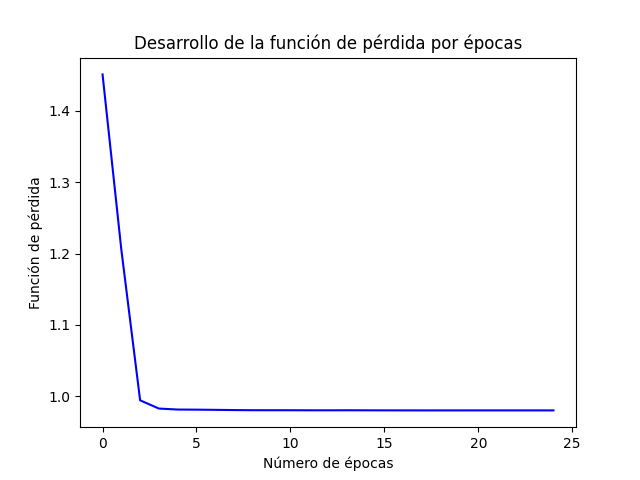
\includegraphics[scale=0.75]{imagenes/loss_autoencoder_fully_connected.png}
	\caption{Evolución de la función de pérdida para el Autoencoder totalmente conectado.}
	\label{img:loss-autoencoder-fully-connected}
\end{figure}

Como podemos ver el valor de la función de pérdida empieza cercano a $1.5$ y consigue descender alrededor de $0.9$. El comportamiento del modelo es como el que queremos ver, empezamos con un valor alto de la función de pérdida y se observa una reducción de su valor. Tras esta reducción considerable podemos ver una estabilización de la misma cuando seguimos aumentando el número de épocas, por lo que podemos deducir que el número de épocas de entrenamiento es suficiente.

Veamos ahora la gráfica del modelo Autoencoder totalmente conectado por lotes:
\begin{figure}[H]
	\centering
	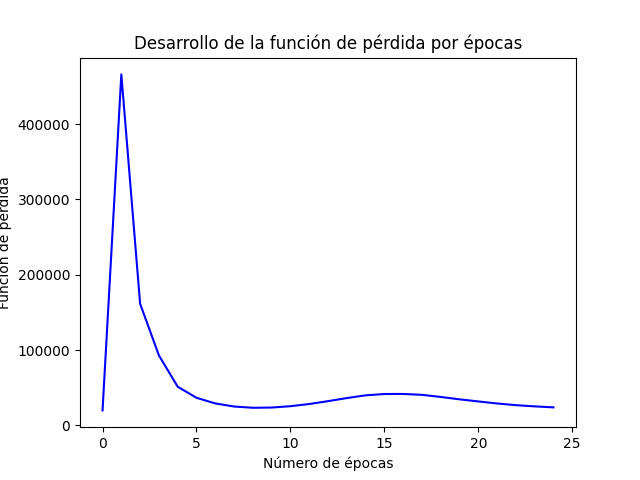
\includegraphics[scale=0.75]{imagenes/loss_autoencoder_fully_connected_batch.png}
	\caption{Evolución de la función de pérdida para el Autoencoder totalmente conectado por lotes.}
	\label{img:loss-autoencoder-fully-connected-batch}
\end{figure}

En este caso podemos ver un comportamiento irregular. En primer lugar podemos ver cómo la primera época (por la inicialización aleatoria de pesos) obtiene una buena loss, luego sube su valor y empieza un descenso suavizado estabilizándose al final. Lo extraño de este comportamiento es que no se estabiliza completamente, ya que tenemos una pequeña crecida y luego una bajada. Además lo peor de todo lo que podemos observar es el valor tan alto de loss que tenemos. Tenemos un valor enorme de la función de pérdida, posiblemente debido a que no estamos consiguiendo que la red aprenda lo suficiente, ya que esto implica que el error acumulado en la reconstrucción de toda la secuencia es muy alto. Se ha probado con secuencias más bajas de tamaño y es claro que el error se reduce hasta bajar a una única instancia, imitando por tanto el comportamiento del modelo anterior. Esto nos puede indicar que este modelo no será muy efectivo en la detección de eventos anómalos, lo veremos en siguientes secciones.

Ahora vamos a ver el aprendizaje del Autoencoder con capas LSTM:
\begin{figure}[H]
	\centering
	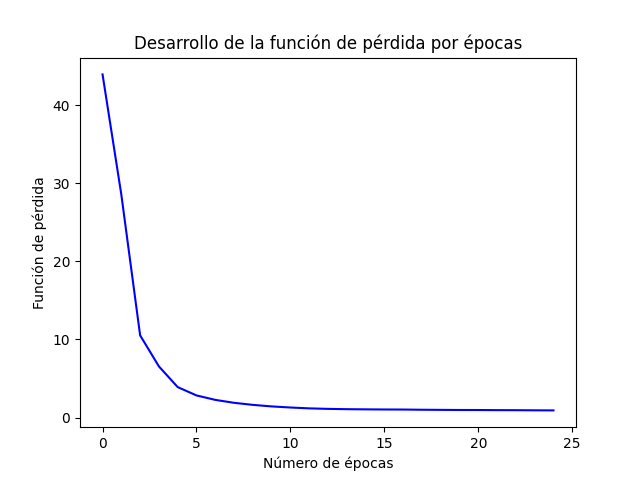
\includegraphics[scale=0.75]{imagenes/loss_autoencoder_lstm.png}
	\caption{Evolución de la función de pérdida para el Autoencoder LSTM.}
	\label{img:loss-autoencoder-lstm}
\end{figure}

De nuevo en este modelo podemos ver un comportamiento adecuado al que buscamos. Empezamos con un valor de la función de pérdida mayor que 40, acabando en un valor cercano a $0.9$ de nuevo. Podemos ver que la progresión en las 5 primeras épocas es muy notoria, reduciéndose el valor de la función de pérdida por debajo de 5. Tras esto se va teniendo una pendiente menos pronunciada hasta que vemos como al final se estabiliza la reducción de la loss. Este comportamiento nos está diciendo que el modelo es capaz de aprender y que además el número de épocas empleadas en el aprendizaje es adecuado.

Ahora veremos la gráfica correspondiente al modelo de predicción CNN-LSTM:
\begin{figure}[H]
	\centering
	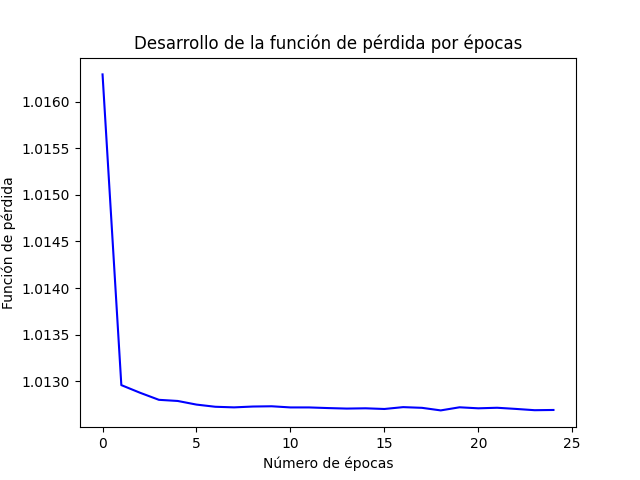
\includegraphics[scale=0.75]{imagenes/loss_cnn_lstm_forecaster.png}
	\caption{Evolución de la función de pérdida para el predictor CNN-LSTM.}
	\label{img:loss-cnn-lstm-forecaster}
\end{figure}

Podemos ver en este caso que los valores de la función de pérdida empiezan bajos, aún así continúan reduciéndose y se estabilizan al final. Con esta gráfica podemos ver que el aprendizaje del modelo es adecuado, ya que consigue una buena loss y se estabilizan los valores, indicando que el número de épocas es suficiente. El valor final de la función de pérdida queda finalmente alrededor de 1.

Por último veamos la gráfica del modelo de predicción LSTM:
\begin{figure}[H]
	\centering
	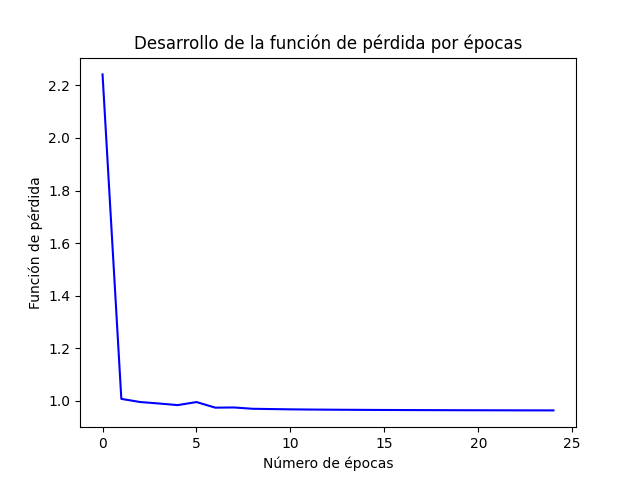
\includegraphics[scale=0.75]{imagenes/loss_lstm_forecasting.png}
	\caption{Evolución de la función de pérdida para el predictor LSTM.}
	\label{img:loss-lstm-forecaster}
\end{figure}

Como podemos ver en este caso también, tenemos un buen aprendizaje del modelo, pues podemos observar una reducción del valor de la función de pérdida desde más de $2.2$ hasta algo maś de $0.9$. Además, podemos ver una reducción muy fuerte de la loss en las primeras etapas y cómo después se estabiliza y se produce muy poca reducción o ninguna. Todo esto nos dice que el modelo ha sido capaz de aprender y además, que el número de épocas empleadas es suficiente para llegar al límite de aprendizaje del modelo o acercarnos al mismo.

Lo siguiente que vamos a hacer es analizar los resultados obtenidos por los modelos con la intención de evaluar la calidad de los mismos y poder discernir el que mejor se comporta de todos ellos.

\section{Resultados obtenidos}

Lo primero que vamos a hacer es ver los resultados de verdaderos positivos, falsos positivos y mantenimientos detectados. En el periodo de prueba que hemos escogido tenemos 28 mantenimientos totales que podemos detectar. Es claro que nos interesa detectar cuantos más mantenimientos mejor, pero si tenemos un modelo que a cambio nos da muchos falsos positivos no es una buena elección. Por poner un ejemplo evidente, si tenemos un modelo que siempre da alerta entonces va a detectar todos los mantenimientos, pero también va a tener un número muy elevado de falsos positivos.

Por ello el mejor modelo no podemos elegirlo sólo en base al número de mantenimientos que detectamos sobre el total, tendremos que sopesar también el resto de métricas. Por tanto veamos ahora la tabla de resultados:

\begin{table}[H]
	\centering
	\begin{tabular}{|l|c|c|c|c|}
		\hline
		\multicolumn{1}{|c|}{\textbf{Modelo}} & \textbf{TP} & \textbf{FP} & \textbf{Mant. Detectados} & \textbf{Mant. Totales} \\ \hline
		\textbf{AE FCC}                       & 33          & 441         & 20                                 & 28                              \\ \hline
		\textbf{AE FCC lotes}                 & 33          & 393         & 20                                 & 28                              \\ \hline
		\textbf{AE LSTM}                      & 33          & 447         & 20                                 & 28                              \\ \hline
		\textbf{Predictor LSTM}               & 33          & 393         & 20                                 & 28                              \\ \hline
		\textbf{Predictor CNN-LSTM}           & 35          & 213         & 22                                 & 28                              \\ \hline
		\textbf{FB LOF}                       & 15          & \textbf{56} & 8                                  & 28                              \\ \hline
		\textbf{HBOS}                         & \textbf{44} & 505         & \textbf{23}                        & 28                              \\ \hline
		\textbf{IForest}                      & 28          & 344         & 19                                 & 28                              \\ \hline
		\textbf{KNN}                          & 42          & 505         & \textbf{23}                        & 28                              \\ \hline
		\textbf{LODA}                         & 36          & 341         & 22                                 & 28                              \\ \hline
		\textbf{LOF}                          & 40          & 471         & 22                                 & 28                              \\ \hline
		\textbf{PCA}                          & 26          & 256         & 16                                 & 28                              \\ \hline
	\end{tabular}
	\caption{Tabla de resultados generales de los modelos a comparar.}
	\label{tabla:resultados1}
\end{table}

La primera métrica que tenemos que observar en esta tabla es la de mantenimientos detectados. Podemos ver que en total tenemos 28 mantenimientos y tenemos dos métodos con 23 mantenimientos detectados y tres con 22 mantenimientos detectados. Entre estos, si no tuviéramos más información, lo lógico es decir que los mejores modelos son aquellos que más mantenimientos detectan. Sabiendo lo que hemos discutido anteriormente esto no es así, ya que debemos intentar también maximizar los verdaderos positivos (cuantos más verdaderos positivos tengamos más certeza tenemos de la detección de los mantenimientos) y minimizar los falsos positivos.

A la vista está que todos los modelos tienen un alto número de falsos positivos, pero vamos a intentar ver cuáles tienen mejores números entre los considerados. Por supuesto la intención es maximizar los verdaderos positivos y minimizar los falsos positivos. Los dos modelos que más mantenimientos predicen correctamente podemos ver que tienen 505 falsos positivos ambos. Esto es una cifra altísima, que nos está indicando que casi siempre dan alerta y por tanto aciertan más mantenimientos a costa de fallar mucho más en las zonas normales. Por contra, podemos ver que LOF y LODA cometen algunos menos falsos positivos sólo fallando un mantenimiento más, pero el mejor de todos en este sentido es el predictor CNN-LSTM que baja los falsos positivos a 213, menos de la mitad de los que cometen HBOS y KNN sólo por un mantenimiento más.

Es por esto que, con estas métricas, podemos decir que el modelo de predicción CNN-LSTM se comporta mejor que el resto ya que consigue predecir 22 de los 28 mantenimientos con 35 verdaderos positivos y sólo 213 falsos positivos. En la métrica de los falsos positivos es el que menos fallos comete después del modelo Feature Bagging LOF, que sólo tiene 56 falsos positivos pero predice correctamente únicamente 8 mantenimientos de los 28. 

Este problema no es un problema de clasificación al uso, aunque podemos intentar convertirlo en un problema de clasificación de dos clases. Cuando damos alerta y hay un mantenimiento cerca tenemos un verdadero positivo, cuando tenemos un mantenimiento cerca pero no damos alerta tenemos un falso negativo, cuando no tenemos mantenimiento cerca y damos la alerta tenemos un falso positivo y si no tenemos un mantenimiento cerca y no damos la alerta entonces tenemos un verdadero negativo. Con esta distribución podemos sacar la matriz de confusión clásica de un problema de dos clases con TP, TN, FP y FN, por lo que podemos sacar algunas métricas más.

\begin{table}[H]
	\centering
	\begin{tabular}{|l|c|c|c|c|}
		\hline
		\multicolumn{1}{|c|}{\textbf{Modelo}} & \textbf{TP} & \textbf{FP} & \textbf{TN}  & \textbf{FN} \\ \hline
		\textbf{AE FCC}                       & 33          & 441         & 75           & 8           \\ \hline
		\textbf{AE FCC lotes}                 & 33          & 393         & 123          & 8           \\ \hline
		\textbf{AE LSTM}                      & 33          & 447         & 69           & 8           \\ \hline
		\textbf{Predictor LSTM}               & 33          & 393         & 123          & 8           \\ \hline
		\textbf{Predictor CNN-LSTM}           & 35          & 213         & 301          & 8           \\ \hline
		\textbf{FB LOF}                       & 15          & \textbf{56} & \textbf{340} & 20          \\ \hline
		\textbf{HBOS}                         & \textbf{44} & 505         & 0            & \textbf{5}  \\ \hline
		\textbf{IForest}                      & 28          & 344         & 177          & 9           \\ \hline
		\textbf{KNN}                          & 42          & 505         & 1            & \textbf{5}  \\ \hline
		\textbf{LODA}                         & 36          & 341         & 172          & 6           \\ \hline
		\textbf{LOF}                          & 40          & 471         & 38           & 6           \\ \hline
		\textbf{PCA}                          & 26          & 256         & 267          & 12          \\ \hline
	\end{tabular}
	\caption{Tabla con los verdaderos positivos, falsos positivos, verdaderos negativos y falsos negativos.}
	\label{tabla:resultados2}
\end{table}

Estamos ante un problema de clasificación con dos clases muy desbalanceado, como podemos suponer. Está claro que vamos a tener un número mucho mayor de zonas sin alerta real (no están cerca de un mantenimiento) que zonas en las que deberíamos de dar la alerta. Además, también está claro que es más valioso para la empresa detectar las alertas que las zonas normales ya que las alertas implican la parada de la maquinaria y por tanto una pérdida de tiempo de trabajo y dinero.

Teniendo esto claro, la tabla \ref{tabla:resultados2} nos refleja el desempeño de los modelos al intentar predecir las alertas de mantenimiento y las zonas normales. Lo que vamos a querer es maximizar los verdaderos positivos y verdaderos negativos e intentar minimizar los falsos positivos y falsos negativos.

Como podemos observar en la tabla, el modelo que menos falsos positivos comete y más verdaderos negativos tiene es Feature Bagging LOF. En la tabla anterior comentamos el posible comportamiento de este modelo, pero ahora lo podemos tener algo más claro. El modelo no da la alerta casi nunca y por tanto predice correctamente muy pocos mantenimientos, por contra al no dar muchas alarmas, es capaz de detectar correctamente muchos periodos normales. Este comportamiento no nos es nada útil pues estamos primando la detección de la normalidad frente a las anomalías.

Por otro lado, podemos ver que el modelo que más verdaderos positivos da es HBOS con 44. Además este modelo es el que menos falsos negativos nos produce junto con el modelo KNN. Lo interesante de esta tabla es que, si quitamos el modelo Feature Bagging LOF de la ecuación, el predictor CNN-LSTM es el que más verdaderos negativos tiene y el que menos falsos positivos tiene entre todos los modelos considerados. Esto junto con el hecho de que no tiene muchos menos verdaderos positivos que HBOS ni muchos más falsos negativos hace que sea un modelo más equilibrado.

En este problema tenemos dos formas de calcular el acierto de los modelos: podemos calcular el porcentaje de mantenimientos detectados y podemos calcular el acierto de verdaderos positivos y verdaderos negativos sobre el total. La segunda de las formas lo que pretende es que, el modelo con acierto perfecto debería de ser capaz de dar alarma en todas las ventanas temporales que caigan 6 horas antes de un mantenimiento y debería ser capaz de no dar ninguna alarma en el resto de ventanas temporales. Por tanto estaríamos calculando el porcentaje de acierto sobre las ventanas temporales y no sobre los mantenimientos directamente.

\begin{table}[H]
	\centering
	\begin{tabular}{|l|c|c|}
		\hline
		\multicolumn{1}{|c|}{\textbf{Modelo}} & \textbf{\begin{tabular}[c]{@{}c@{}}Tasa mantenimientos\\ detectados\end{tabular}} & \textbf{\begin{tabular}[c]{@{}c@{}}Acierto sobre\\ ventanas\end{tabular}} \\ \hline
		\textbf{AE FCC}                       & 0.7143                                                                            & 0.1939                                                                    \\ \hline
		\textbf{AE FCC lotes}                 & 0.7143                                                                            & 0.2801                                                                    \\ \hline
		\textbf{AE LSTM}                      & 0.7143                                                                            & 0.1831                                                                    \\ \hline
		\textbf{Predictor LSTM}               & 0.7143                                                                            & 0.2801                                                                    \\ \hline
		\textbf{Predictor CNN-LSTM}           & 0.7857                                                                            & 0.6054                                                                    \\ \hline
		\textbf{FB LOF}                       & 0.2857                                                                            & \textbf{0.8237}                                                           \\ \hline
		\textbf{HBOS}                         & \textbf{0.8214}                                                                   & 0.0794                                                                    \\ \hline
		\textbf{IForest}                      & 0.6786                                                                            & 0.3674                                                                    \\ \hline
		\textbf{KNN}                          & \textbf{0.8214}                                                                   & 0.0794                                                                    \\ \hline
		\textbf{LODA}                         & 0.7857                                                                            & 0.3748                                                                    \\ \hline
		\textbf{LOF}                          & 0.7857                                                                            & 0.1405                                                                    \\ \hline
		\textbf{PCA}                          & 0.5714                                                                            & 0.5223                                                                    \\ \hline
	\end{tabular}
	\caption{Tabla con los aciertos de los modelos.}
	\label{tabla:resultados3}
\end{table}

En la columna de tasa de mantenimientos detectados vemos que no tenemos ninguna sorpresa, ya que lo hemos analizado previamente cuando hemos visto el número de mantenimientos que detectaba cada uno de los modelos. En la columna de acierto sobre ventanas tenemos alguna sorpresa más. Como podemos ver el modelo que mejor resultado da es Feature Bagging LOF, lo cual es razonable. Ya hemos comentado que hay muchas más ventanas en zonas de normalidad que en zonas anómalas, por lo que el modelo, al no dar casi alarmas, acierta casi todas las ventanas. Si eliminamos este modelo de la ecuación podemos ver que el siguiente mejor modelo es el predictor CNN-LSTM. Esta tabla nos está diciendo que deberíamos emplear alguna métrica de problemas de clasificación desbalanceada para poder comparar mejor los aciertos, por tanto vamos a ver la tasa de positivos y negativos y vamos a utilizar la multiplicación de las mismas como métrica.

\begin{table}[H]
	\centering
	\begin{tabular}{|l|c|c|l|}
		\hline
		\multicolumn{1}{|c|}{\textbf{Modelo}} & \textbf{TPR}    & \textbf{TNR}    & \multicolumn{1}{c|}{\textbf{TPRxTNR}} \\ \hline
		\textbf{AE FCC}                       & 0.8049          & 0.1453          & 0.1170                                \\ \hline
		\textbf{AE FCC lotes}                 & 0.8049          & 0.2384          & 0.1919                                \\ \hline
		\textbf{AE LSTM}                      & 0.8049          & 0.1337          & 0.1076                                \\ \hline
		\textbf{Predictor LSTM}               & 0.8049          & 0.2384          & 0.1919                                \\ \hline
		\textbf{Predictor CNN-LSTM}           & 0.8537          & 0.5856          & \textbf{0.5}                          \\ \hline
		\textbf{FB LOF}                       & 0.4286          & \textbf{0.8586} & 0.3680                                \\ \hline
		\textbf{HBOS}                         & \textbf{0.8980} & 0               & 0                                     \\ \hline
		\textbf{IForest}                      & 0.7568          & 0.3397          & 0.2571                                \\ \hline
		\textbf{KNN}                          & 0.8959          & 0.0020          & 0.0018                                \\ \hline
		\textbf{LODA}                         & 0.8571          & 0.3353          & 0.2874                                \\ \hline
		\textbf{LOF}                          & 0.8696          & 0.0747          & 0.0649                                \\ \hline
		\textbf{PCA}                          & 0.6842          & 0.5105          & 0.3493                                \\ \hline
	\end{tabular}
	\caption{Tabla con las tasas de positivos y negativos.}
	\label{tabla:resultados4}
\end{table}

En esta tabla podemos ver la tasa de acierto de positivos, la de negativos y la multiplicación de ambas. La intención de multiplicar ambas tasas es que podemos tener una buena puntuación en alguna de ellas pero muy mala en la otra. Esto nos estaría diciendo que nuestro modelo está desequilibrado y por tanto predice mejor los positivos o los negativos únicamente. 

Esto se puede ver claramente. Parecía que el mejor modelo hasta ahora podía ser HBOS pero podemos ver que la tasa de acierto de negativos es 0, por lo que el modelo está altamente desbalanceado y la tasa al multiplicar sale cero. Por otro lado Feature Bagging LOF podemos ver que acierta muchos negativos, pero falla muchos positivos que son los más importantes. En el caso de KNN y LOF podemos ver que tienen muy buenas tasas de acierto de positivos pero pésimas tasas de acierto de negativos y finalmente podemos ver que LODA tiene algo más de equilibrio, pero el mejor modelo ahora es el predictor CNN-LSTM que es el que mejor puntuación saca al multiplicar las dos tasas de acierto. Esto nos está diciendo que es el más equilibrado de todos con una tasa de acierto en los positivos de un $85.37\%$ y en negativos de un $58.56\%$.

\begin{table}[H]
	\centering
	\begin{tabular}{|l|c|c|}
		\hline
		\multicolumn{1}{|c|}{\textbf{Modelo}} & \textbf{F1}     & \textbf{AUC}  \\ \hline
		\textbf{AE FCC}                       & 0.1282          & 0.48          \\ \hline
		\textbf{AE FCC lotes}                 & 0.1413          & 0.52          \\ \hline
		\textbf{AE LSTM}                      & 0.1267          & 0.47          \\ \hline
		\textbf{Predictor LSTM}               & 0.1413          & 0.52          \\ \hline
		\textbf{Predictor CNN-LSTM}           & 0.2422          & \textbf{0.72} \\ \hline
		\textbf{FB LOF}                       & \textbf{0.2830} & 0.64          \\ \hline
		\textbf{HBOS}                         & 0.1471          & 0.45          \\ \hline
		\textbf{IForest}                      & 0.1369          & 0.55          \\ \hline
		\textbf{KNN}                          & 0.1443          & 0.45          \\ \hline
		\textbf{LODA}                         & 0.1718          & 0.6           \\ \hline
		\textbf{LOF}                          & 0.1436          & 0.47          \\ \hline
		\textbf{PCA}                          & 0.1625          & 0.6           \\ \hline
	\end{tabular}
	\caption{Tabla de resultados con F1 y AUC.}
	\label{tabla:resultados5}
\end{table}

La medida F1 nos mide el número de verdaderos positivos que tenemos en relación a la media de falsos positivos y falsos negativos, por lo que cuanto más alto sea el valor y más cercano a 1 mejor será el modelo. En este caso tenemos claro que cometemos muchos falsos positivos, por lo que los modelos sufren una penalización muy grande en esta métrica. Podemos ver que Feature Bagging LOF es el que mejores números obtiene en esta métrica, pero ya sabemos que no es comparable. El siguiente modelo es el predictor CNN-LSTM, por lo que podemos decir que este modelo es el mejor en esta métrica. 

En la siguiente columna tenemos el AUC o Área Bajo la Curva ROC en este caso. La curva ROC es una curva en la que contraponemos en el eje X la tasa de falsos positivos y en el eje Y la tasa de verdaderos positivos variando el umbral probabilístico en el que consideramos que tenemos un positivo o un negativo. En este caso no podemos variar este umbral, por lo que sólo vamos a tener un punto. A mayor área bajo esta curva mejor y cuanto más cercano sea el punto de la curva al $(1,0)$ mejor. Por tanto en el mejor de los casos la curva ROC será la parte superior de un cuadrado y el AUC 1, mientras que en el peor de los casos también tendremos AUC 1 pero tendremos ahora la curva ROC el lado inferior del cuadrado. Veamos por tanto las gráficas ROC:

\begin{figure}[H]
	\centering
	\begin{subfigure}{.49\textwidth}
		\centering
		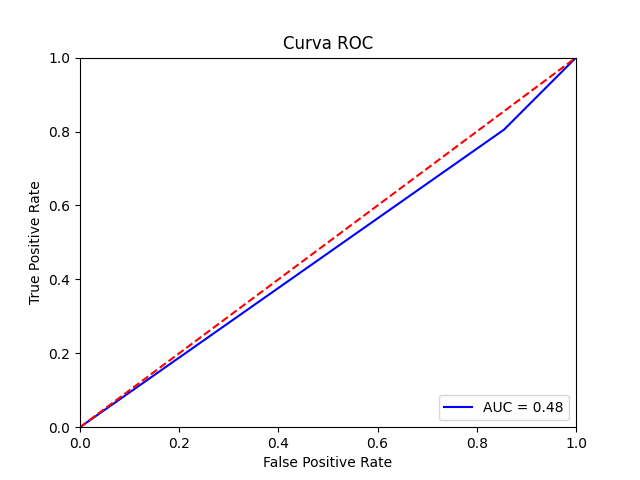
\includegraphics[scale=0.42]{imagenes/roc/Autoencoder-Fully-Connected_roc.png}
		\caption{Autoencoder totalmente conectado.}
	\end{subfigure}
	\begin{subfigure}{.49\textwidth}
		\centering
		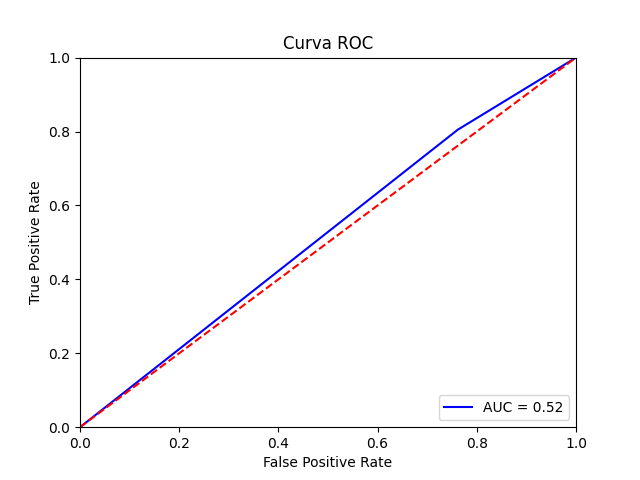
\includegraphics[scale=0.42]{imagenes/roc/Autoencoder-Fully-Connected-Lotes_roc.png}
		\caption{Autoencoder totalmente conectado por lotes.}
	\end{subfigure}
	\label{img:roc1}
\end{figure}

\begin{figure}[H]
	\centering
	\begin{subfigure}{.49\textwidth}
		\centering
		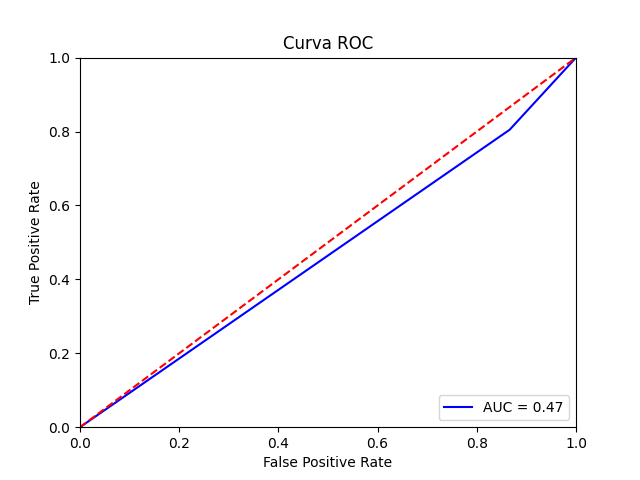
\includegraphics[scale=0.42]{imagenes/roc/Autoencoder-LSTM_roc.png}
		\caption{Autoencoder LSTM.}
	\end{subfigure}
	\begin{subfigure}{.49\textwidth}
		\centering
		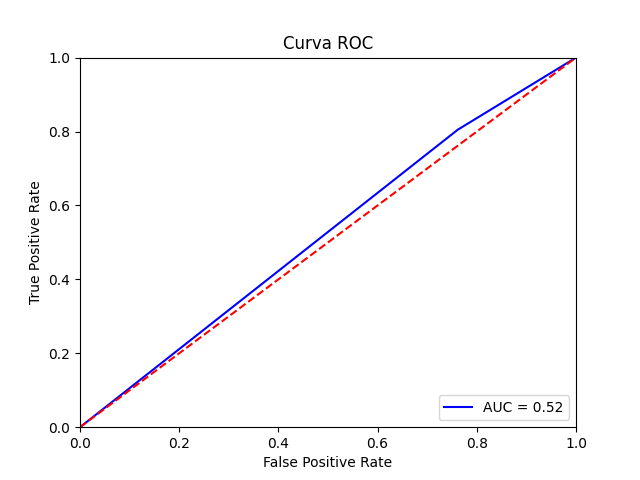
\includegraphics[scale=0.42]{imagenes/roc/Predictor-LSTM_roc.png}
		\caption{Modelo de predicción LSTM.}
	\end{subfigure}
	\label{img:roc2}
\end{figure}

\begin{figure}[H]
	\centering
	\begin{subfigure}{.49\textwidth}
		\centering
		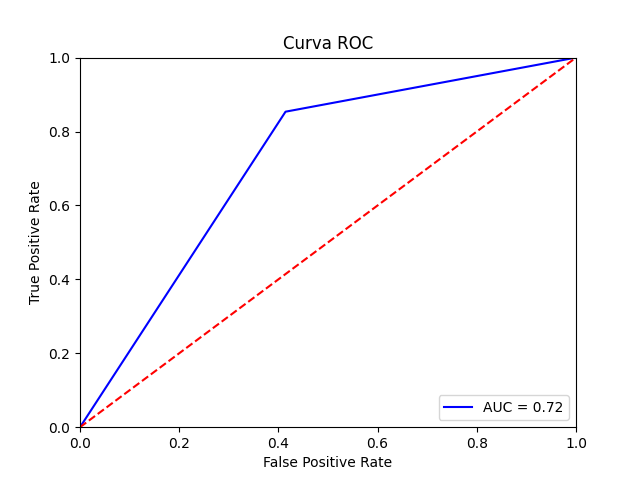
\includegraphics[scale=0.42]{imagenes/roc/Predictor-CNN-LSTM_roc.png}
		\caption{Predictor CNN-LSTM.}
	\end{subfigure}
	\begin{subfigure}{.49\textwidth}
		\centering
		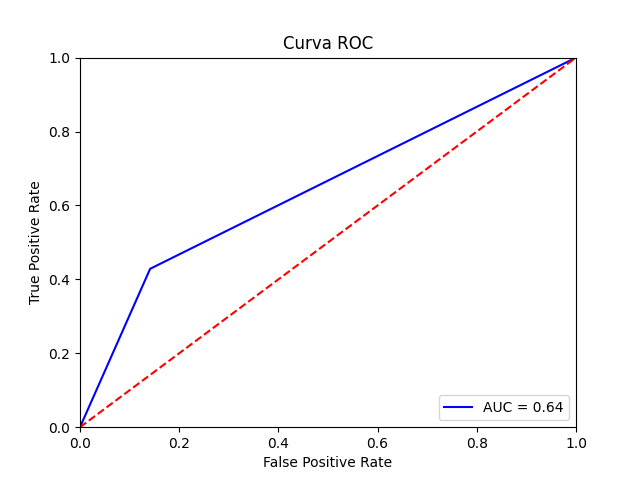
\includegraphics[scale=0.42]{imagenes/roc/Feature-Bagging-LOF_roc.png}
		\caption{Feature Bagging LOF.}
	\end{subfigure}
	\label{img:roc3}
\end{figure}

\begin{figure}[H]
	\centering
	\begin{subfigure}{.49\textwidth}
		\centering
		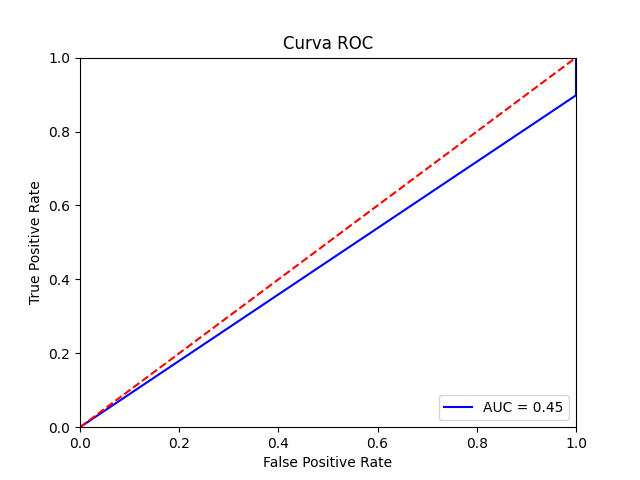
\includegraphics[scale=0.42]{imagenes/roc/HBOS_roc.png}
		\caption{HBOS.}
	\end{subfigure}
	\begin{subfigure}{.49\textwidth}
		\centering
		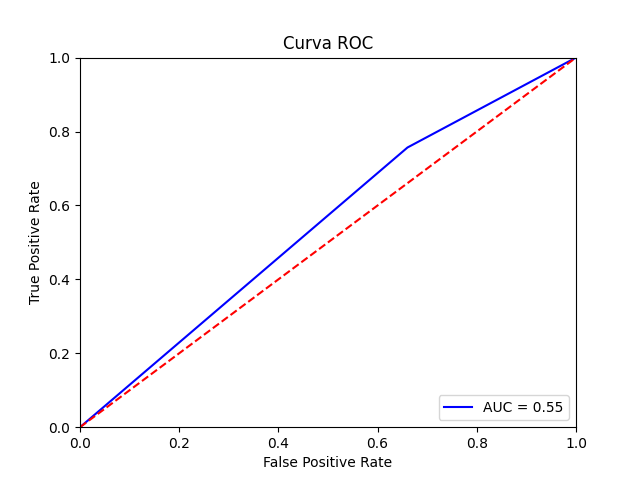
\includegraphics[scale=0.42]{imagenes/roc/Isolation-Forest_roc.png}
		\caption{Isolation Forest.}
	\end{subfigure}
	\label{img:roc4}
\end{figure}

\begin{figure}[H]
	\centering
	\begin{subfigure}{.49\textwidth}
		\centering
		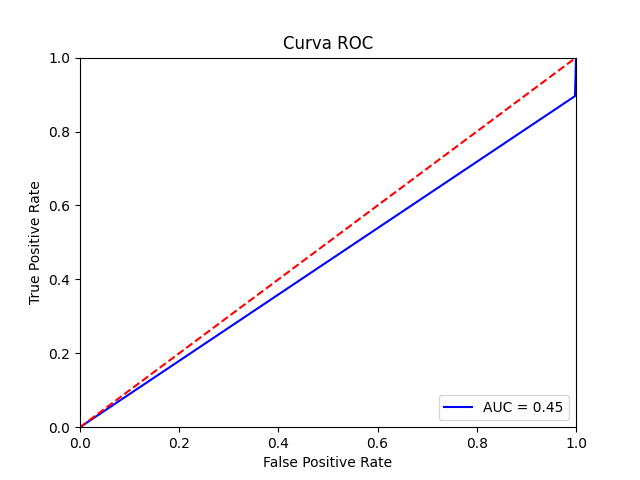
\includegraphics[scale=0.42]{imagenes/roc/KNN_roc.png}
		\caption{KNN.}
	\end{subfigure}
	\begin{subfigure}{.49\textwidth}
		\centering
		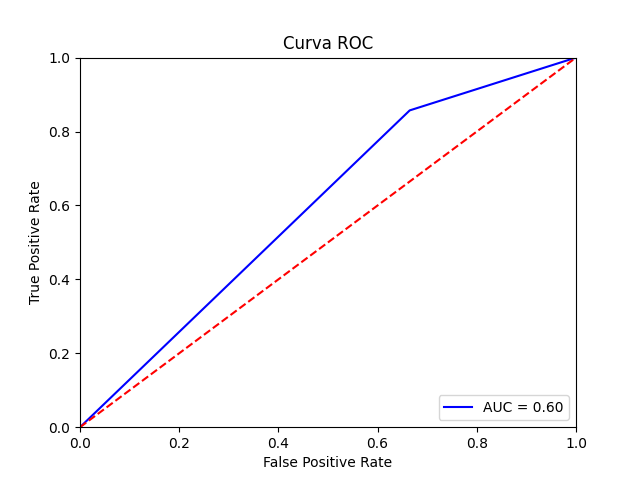
\includegraphics[scale=0.42]{imagenes/roc/LODA_roc.png}
		\caption{LODA.}
	\end{subfigure}
	\label{img:roc5}
\end{figure}

\begin{figure}[H]
	\centering
	\begin{subfigure}{.49\textwidth}
		\centering
		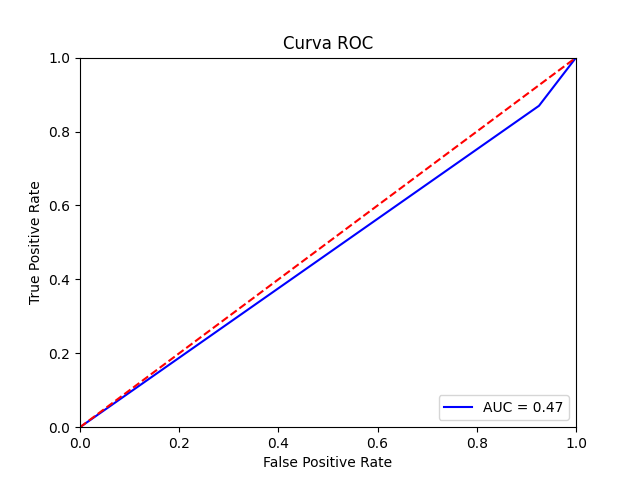
\includegraphics[scale=0.42]{imagenes/roc/LOF_roc.png}
		\caption{LOF.}
	\end{subfigure}
	\begin{subfigure}{.49\textwidth}
		\centering
		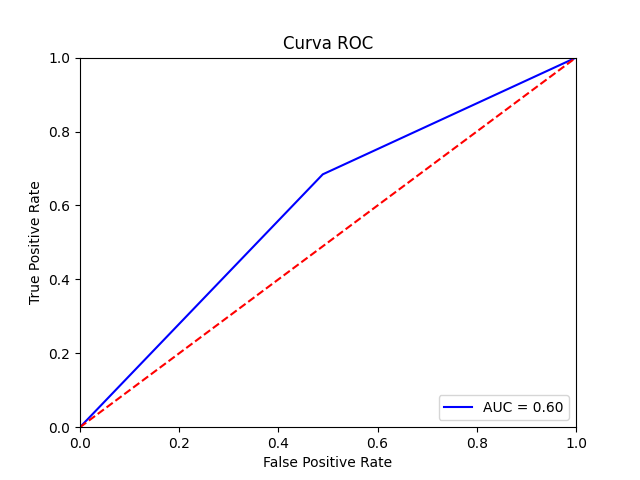
\includegraphics[scale=0.42]{imagenes/roc/PCA_roc.png}
		\caption{PCA.}
	\end{subfigure}
	\label{img:roc6}
\end{figure}

En las gráficas podemos ver que tenemos una línea roja discontinua en medio. Esta línea nos marca el comportamiento de un modelo aleatorio, que tendría la misma efectividad que lanzar una moneda al aire y discernir la clase de forma aleatoria según una uniforme. La intención es que los mejores modelos estén por encima de esta línea y si el modelo está por debajo es que es peor que un modelo aleatorio.

Podemos ver que el mejor de los modelos según la curva ROC es el predictor CNN-LSTM con un AUC de $0.72$. Por contra aquí podemos ver que la tasa de falsos positivos hace que los modelos KNN y HBOS tengan las peores curvas ROC de todas. En cuanto al modelos FeatureBagging LOF hemos visto ya que no acierta lo suficiente como para tenerlo en consideración y podemos ver que PCA tiene un comportamiento razonablemente equilibrado pero sólo predicen correctamente 16 de los 28 mantenimientos por lo que no está a la altura del resto de modelos. Por otro lado tenemos a LODA que tiene un comportamiento razonablemente bueno pero es peor aún así que el predictor CNN-LSTM.

Por tanto de nuevo hemos podido ver que el modelo de predicción CNN-LSTM es el modelo que mejor resultado nos ha arrojado en estas métricas.

Por último vamos a comparar los tiempos de los modelos. Hay que recordar que los modelos clásicos de detección de anomalías no tienen un periodo de entrenamiento pues no hay etiquetas de las que aprender. En cambio en los modelos Deep Learning si que tenemos un periodo de entrenamiento que vamos a comparar ahora entre modelos:

\begin{figure}[H]
	\centering
	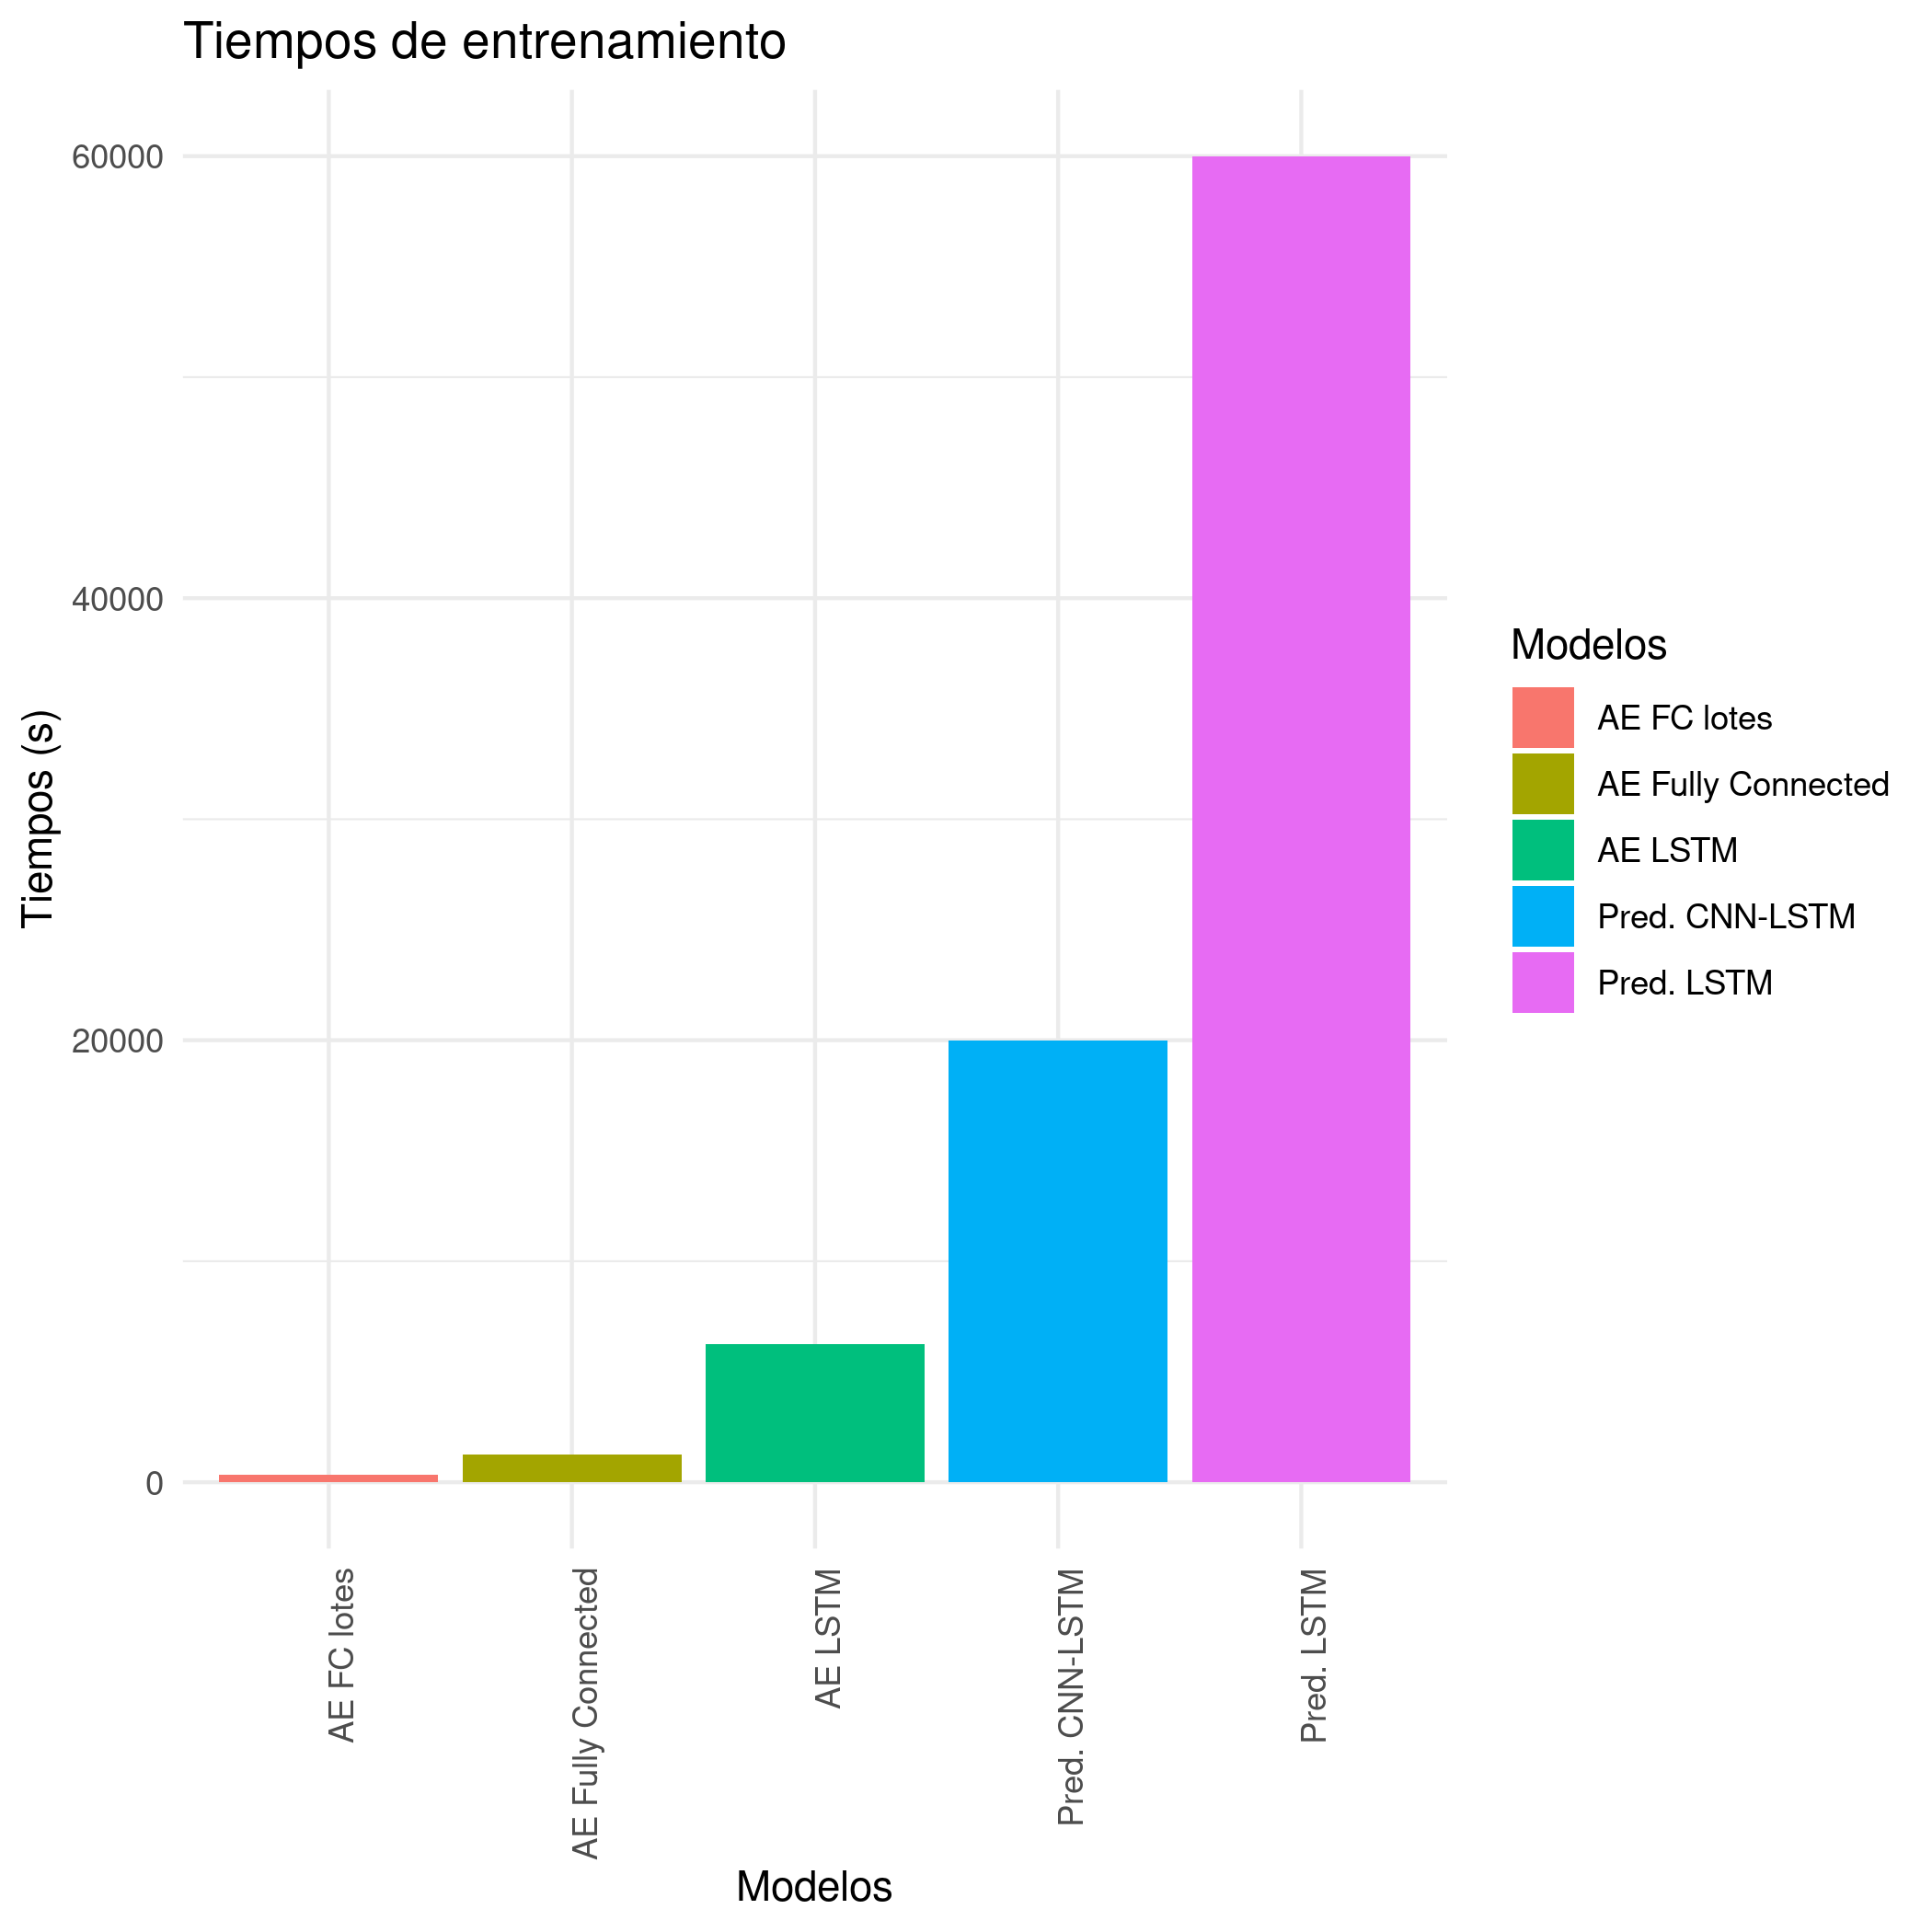
\includegraphics[scale=0.65]{imagenes/tiempos_entrenamiento.png}
	\caption{Tiempos de entrenamiento modelos Deep Learning.}
	\label{img:tiempos-entrenamiento}
\end{figure}

Aquí podemos ver que los modelos tienen tiempos de entrenamiento muy distintos. En primer lugar todos los modelos Autoencoder tienen tiempos de entrenamiento bastante bajos, mientras que los modelos de predicción tienen tiempos de entrenamiento mucho más altos. En particular podemos ver cómo los modelos totalmente conectados son los que menor tiempo de entrenamiento tienen mientras que el que más es el modelo de predicción puramente LSTM.

Este tiempo es importante pero sólo vamos a tener que entrenar por completo un modelo una vez, por lo que lo que más nos interesa es cuánto tardamos en predecir un día completo de datos. Estos tiempos hacen referencia a cuánto tardamos en obtener los scores del modelo, no en el proceso completo. No necesitamos saber cuánto tardamos en el resto del proceso para comparar los modelos, pues las operaciones siempre son las mismas a partir de tener los scores. Los tiempos que varían son los que cada modelo consume para poder sacar las puntuaciones de anomalía, veamos las gráficas por tanto:

\begin{figure}[H]
	\centering
	\includegraphics[scale=0.65]{imagenes/tiempos_prediccion.png}
	\caption{Tiempos de predicción de los modelos.}
	\label{img:tiempos-prediccion}
\end{figure}

Podemos ver que el modelo que más tiempo consume (dando malos resultados) es el modelo Feature Bagging LOF que nos está distorsionando un poco la escala de la gráfica. Ya que hemos comprobado que su desempeño en tiempo es malo vamos a eliminarlo de la misma para poder ver mejor el resto de modelos:

\begin{figure}[H]
	\centering
	\includegraphics[scale=0.65]{imagenes/tiempos_prediccion2.png}
	\caption{Tiempos de predicción de los modelos sin Feature Bagging LOF.}
	\label{img:tiempos-prediccion2}
\end{figure}

Aquí podemos ver algo mejor los tiempos que consumen los algoritmos en predecir. Podemos ver que LOF y KNN son los que maś tiempo consumen en predecir, por encima de 90 segundos. Por otro lado tenemos Isolation Forest después de estos con alrededor ed 40-45 segundos. Tras esto vienen el resto de modelos con unos tiempos mucho más bajos, todos con 10 segundos o menos en predecir un día de datos completo. 

Cabe decir que, por tiempo consumido, todos los modelos son viables en el uso para esta tarea, pero podemos ver claramente que los modelos Deep Learning consumen muy poco tiempo y en concreto, el modelo de predicción CNN-LSTM consume poco tiempo y es el modelo que mejor resultado nos ha arrojado.

Sobre estas comparativas de tiempos cabe resaltar las máquinas empleadas para los cálculos. Para todos los modelos se ha empleado la misma máquina aunque no siempre el mismo hardware. En el cómputo de los scores de anomalías y en los entrenamientos de los modelos que lo necesiten se ha empleado una máquina DGX-1. Esta máquina dispone de 8 tarjetas gráficas NVIDIA Tesla V100 con 32 GB de memoria, 5120 CUDA cores y 640 Tensor Cores. Posee 512 GB de memoria RAM y 80 núcleos aportados por dos procesadores Intel Xeon E5-2698.

Para el entrenamiento de los modelos Deep Learning se ha empleado una sola tarjeta gráfica al igual que para la predicción de los mismos modelos. Por otro lado, los modelos clásicos que tienen disponible paralelismo se han ejecutado sobre los 80 núcleos de la máquina para aprovechar el potencial al máximo.
%
\chapter{Conclusiones y Trabajo Futuro}
\label{chapter:conclusiones-trabajo-futuro}

En este capítulo vamos a exponer las conclusiones obtenidas del anterior estudio, así como el trabajo futuro directo implicado por las conclusiones y los pasos naturales a seguir.

\section{Conclusiones}

El estudio ha versado sobre la efectividad de algunos métodos de detección de anomalías clásicos sobre un problema no supervisado de mantenimiento predictivo sobre una serie temporal real de una máquina industrial de la compañía ArcelorMittal. El hecho de que el problema sea un problema real y no académico es la posibilidad de ver su utilidad en una aplicación empresarial. Este trabajo ha sido muy enriquecedor y me ha permitido ver el potencial de los modelos Deep Learning sin desprestigiar algunos métodos clásicos de detección de anomalías que permanecen en un nivel de desempeño cercano.

La primera conclusión que podemos sacar de este estudio es que el mejor modelo en desempeño ha resultado ser el modelo de predicción CNN-LSTM. En la sección anterior hemos podido analizar el desempeño de todos los modelos desde el punto de vista de varias métricas para analizar en profundidad los mismos. El modelo de predicción CNN-LSTM ha resultado ser el modelo más equilibrado de todos los analizados así como el mejor modelo en algunas de las métricas que hemos empleado. Además hemos podido ver que su consumo de tiempo en la predicción es muy bajo comparado con el resto de modelos clásicos y Deep Learning.

Lo siguiente que hemos podido ver es que los modelos Deep Learning tienen un buen potencial y merece la pena considerarlos para este tipo de problemas. En concreto hemos podido ver que los dos mejores modelos en desempeño han sido los modelos basados en predicción seguidos por el Autoencoder con capas LSTM. No debemos desechar ninguna de las dos propuestas (predicción y autoencoder) pues han demostrado ambas su potencial.

En cuanto a los modelos clásicos tenemos a HBOS y KNN que nos han dado los mejores resultados entre ellos. Estos resultados están un poco enturbiados por la cantidad de falsos positivos que arrojan, lo que nos dice que tienen tendencia a dar demasiadas alarmas y por tanto aciertan muchos mantenimientos pero dan muchos falsos positivos.

Si comparamos internamente los modelos Deep Learning hemos podido comprobar que los modelos de predicción se comportan mejor que los modelos Autoencoder en general. 

Durante el desarrollo del estudio comentamos que este problema era como un puzle, en el que tenemos nuestro algoritmo de detección de anomalías acompañado del algoritmo de obtención de etiquetas de anomalías y el algoritmo de detección de eventos anómalos que nos alerta de un mantenimiento. En este estudio hemos podido ver cómo las métricas de los modelos han estado muy cerca en algunos casos, lo que nos está indicando que no sólo el modelo es importante, si no que la pieza de detección de eventos anómalos es fundamental y debemos también optimizarla y pensar en ella como algo fundamental.

Finalmente cabe recalcar de nuevo la importancia del estudio. Estamos ante un caso de aplicación real de estos métodos generando utilidad a la empresa. Si somos capaces de detectar los mantenimientos antes de que ocurran estamos indicando cuándo vamos a tener que hacer una parada de la máquina y por tanto podemos evitar algún fallo catastrófico que pare completamente el proceso de producción. Esto se traduce en ahorro de dinero y de tiempo, en consecuencia es un mayor beneficio para la empresa.

\section{Trabajo Futuro}

En esta sección vamos a discutir los pasos naturales a seguir en la evolución de este trabajo. Con lo que hemos conseguido hasta ahora tenemos unos buenos resultados, pero hay mucho que mejorar y posibilidad para ello.

En primer lugar, un problema común a todos los modelos es que arrojan un número excesivo de falsos positivos. Para poder solventar esto tenemos muchos algoritmos que nos ayudan a la mitigación de falsos positivos, como los mencionados en la revisión de Zohrevand y Glässer \cite{zahra_should_2019}. Este es un paso natural y, al afectar a todos los modelos, debemos empezar por este paso para solucionarlo cuanto antes.

El trabajo no tiene una comprobación exhaustiva de los parámetros de los modelos, pues el sistema de cuantificación consume un tiempo elevado y no resulta sencillo automatizarlo. Aún así merece la pena dedicar tiempo a esta tarea y a su cómputo para poder mejorar aún más el desempeño de los modelos y llevarlos al límite. Puede que con este paso consigamos de por sí una reducción de los falsos positivos si los introducimos en la métrica a maximizar.

Por otro lado se ha hecho una revisión de 5 arquitecturas Deep Learning, pero tenemos muchas más que explorar e incluso generalizar aún más las ya propuestas. Por ejemplo no tenemos modelos de encoding-decoding asimétricos o modelos CNN con agrupaciones distintas al máximo o modelos con otros tipos de capas recurrentes como por ejemplo las capas Transformer. Es por esto que merece la pena investigar y estudiar nuevas capas y arquitecturas para poder introducirlas en la comparativa.

Durante este estudio también ha surgido la idea de realizar una nueva arquitectura no supervisada propia de detección de anomalías. Esta arquitectura se basaría en ordenar los datos para formar una imagen con un lote temporal de datos ordenando las variables de forma que pudiéramos hacer convoluciones de dos dimensiones para extraer características y después emplear capas LSTM y capas densas o sólo capas densas para realizar predicciones y/o reconstrucciones de las instancias de datos.

También surge como algo natural integrar un sistema de test y train secuencia. Lo normal es que nuestro modelo pruebe datos en tiempo real y vaya prediciendo sobre los mismos. Una vez que los operarios han etiquetado correctamente el mantenimiento y se añaden los datos a la base de datos, podemos emplearlos en el entrenamiento del modelo. De esta forma estamos constantemente añadiendo nuevos datos al mismo, con lo que si hubiera un cambio de concepto leve pero persistente podemos corregir el modelo. Esta filosofía de trabajo se conoce como Test-Then-Train.

Por último, para poder analizar los verdaderos positivos, falsos positivos, verdaderos negativos y falsos negativos de forma adecuada surge la curiosidad de ver qué pasa si los unimos. Por ejemplo, podemos tener muchos falsos positivos pegados en el tiempo y por tanto podríamos unirlos para poder estudiar todo esto por intervalos completos de tiempo. Cabe la duda de cómo ponderar esto en la métrica (no es lo mismo fallar en un intervalo pequeño que en uno de mayores dimensiones temporales) pero puede resultar muy útil para estudiar los periodos temporales en los que nuestro modelo falla.
%%\chapter{Conclusiones y Trabajos Futuros}
%
%
\nocite{*}
\bibliography{referencias}\addcontentsline{toc}{chapter}{Bibliografía}
\bibliographystyle{unsrt}
%
%\appendix
%\input{apendices/manual_usuario/manual_usuario}
%%\input{apendices/paper/paper}
%\input{glosario/entradas_glosario}
% \addcontentsline{toc}{chapter}{Glosario}
% \printglossary
\chapter*{}
\thispagestyle{empty}

\end{document}
